%% Author: Andrew J. Younge
%% PhD Thesis


\documentclass[oneside,phd,etd]{IUCS}

% Specify the following optional arguments in the square brackets to
% specify the thesis type:
%
%   senior  : Produces the senior thesis preliminary pages (default)
%   honors  : Produces the honors thesis preliminary pages
%   masters : Produces the masters thesis preliminary pages
%   phd     : Produces the PhD dissertation preliminary pages
%
% The default format is appropriate for printing, with blank pages
% inserted after the preliminary pages in twoside mode so you can
% send it directly to a two-sided printer. However, for ETD
% submission the blank pages need to be removed from the final output.
% The following option does this for you:
%
%   etd     : Produces a copy with no blank pages in the preliminary section.
%             Remove this option to produce a version with blank pages inserted
%             for easy double sided printing.
%
% The rest of the class options are the same as the regular book class.
% A few to remember:
%
%   oneside : Produces single sided print layout (recommended for theses less than 50 pages)
%   twoside : Produces single sided print layout (the default if you remove oneside)
%
% The BYUPhys class provides the following macros:
%
%   \makepreliminarypages : Makes the preliminary pages
%   \clearemptydoublepage : same as \cleardoublepage but doesn't put page numbers
%                           on blank intervening pages
%   \singlespace          : switch to single spaced lines
%   \doublespace          : switch to double spaced lines
%
% --------------------------- Load Packages ---------------------------------
% The graphicx package allows the inclusion of figures.  Plain LaTeX and
% pdfLaTeX handle graphics differently. The following code checks which one
% you are compiling with, and switches the graphicx package options accordingly.
\usepackage{ifpdf} \ifpdf 
\usepackage[pdftex]{graphicx} \else 
\usepackage[dvips]{graphicx} \fi

% The fancyhdr package allows you to easily customize the page header.
% The settings below produce a nice, well separated header.
\usepackage{fancyhdr}
  \fancyhead{}
  \fancyhead[LO]{\slshape \rightmark}
  \fancyhead[RO,LE]{\textbf{\thepage}}
  \fancyhead[RE]{\slshape \leftmark}
  \fancyfoot{}
  \pagestyle{fancy}
  \renewcommand{\chaptermark}[1]{\markboth{\chaptername \ \thechapter \ \ #1}{}}
  \renewcommand{\sectionmark}[1]{\markright{\thesection \ \ #1}}
% The caption package allows us to change the formatting of figure captions.
% The commands here change to the suggested caption format: single spaced and a bold tag
\usepackage[margin=0.3in,labelfont=bf,labelsep=none]{caption} \DeclareCaptionFormat{suggested}{\singlespace#1#2 #3\par\doublespace} \captionsetup{format=suggested}

% The cite package cleans up the way citations are handled.  For example, it
% changes the citation [1,2,3,6,7,8,9,10,11] into [1-3,6-11].  If your advisor
% wants superscript citations, use the overcite package instead of the cite package.
\usepackage{cite}

% The makeidx package makes your index for you.  To make an index entry,
% go to the place in the book that should be referenced and type
%  \index{key}
% An index entry labeled "key" (or whatever you type) will then
% be included and point to the correct page.
\usepackage{makeidx} 
\makeindex

% The url package allows for the nice typesetting of URLs.  Since URLs are often
% long with no spaces, they mess up line wrapping.  The command \url{http://www.physics.byu.edu}
% allows LaTeX to break the url across lines at appropriate places: e.g. http://www.
% physics.byu.edu.  This is helpful if you reference web pages.
\usepackage{url} \urlstyle{rm}

% If you have a lot of equations, you might be interested in the amstex package.
% It defines a number of environments and macros that are helpful for mathematics.
% We don't do much math in this example, so we haven't used amstex here.
% The hyperref package provides automatic linking and bookmarking for the table
% of contents, index, equation references, and figure references.  It must be
% included for the BYU Physics class to make a properly functioning electronic
% thesis.  It should be the last package loaded if possible.
%
% To include a link in your pdf use \href{URL}{Text to be displayed}.  If your
% display text is the URL, you probably should use the \url{} command discussed
% above.
%
% To add a bookmark in the pdf you can use \pdfbookmark.  You can look up its usage
% in the hyperref package documentation
\usepackage[bookmarksnumbered,pdfpagelabels=true,plainpages=false,colorlinks=true, linkcolor=black,citecolor=black,urlcolor=blue]{hyperref}

% AJY specific packages
\usepackage{float}
\usepackage{comment}
\usepackage{rotating}
\usepackage{subcaption}
\RequirePackage{lineno}


% ------------------------- Fill in these fields for the preliminary pages ----------------------------
%
% For Senior and honors this is the year and month that you submit the thesis
% For Masters and PhD, this is your graduation date
\Year{2016} \Month{September} \Author{Andrew J. Younge}

% If you have a long title, split it between two lines. The \TitleBottom field defines the second line
% A two line title should be an "inverted pyramid" with the top line longer than the bottom.
\TitleTop{Architectural Principles and Experimentation of}
\TitleBottom{Distributed High Performance Virtual Clusters}
%\TitleBottom{High Performance Virtualization}

% \TitleBottom{}
% Your research advisor
\Advisor{Geoffrey C. Fox, Ph.D}

% The department undergraduate research coordinator
\MemberA{Judy Qiu, Ph.D}

% The representative of the department who will approve your thesis (usually the chair)
\MemberB{Thomas Sterling, Ph.D}

% Fourth member, also known as an observer
\MemberC{D. Martin Swany, Ph.D}


% The title of the department representative
%  \DepRepTitle{Graduate Coordinator}
% The text of your abstract
\Abstract{
With the advent of virtualization and Infrastructure-as-a-Service (IaaS), the broader scientific computing community is considering the use of clouds for their scientific computing needs. This is due to the relative scalability, ease of use, advanced user environment customization abilities, and the many novel computing paradigms available for data-intensive applications. However, a notable performance gap exists between IaaS and typical high performance computing (HPC) resources. This has limited the applicability of IaaS for many potential users, not only for those who look to leverage the benefits of virtualization with traditional scientific computing applications, but also for the growing number of big data scientists whose platforms are unable to build on HPC's advanced hardware resources.

Concurrently, we are at the forefront of a convergence in infrastructure between Big Data and HPC, in which a unified distributed computing architecture could provide computing and storage capabilities for both differing distributed systems use cases. There is the potential to leverage performance and advanced hardware from the HPC community, and provide it in a virtualized infrastructure using High Performance Virtual Clusters. This will not only enable a more diverse user environment within supercomputing applications, but also bring increased performance and capabilities to big data platform services. 

This work proposes to bridge the gap between HPC and cloud infrastructure and enable infrasturcture convergence through a framework for virtual clusters. It begins with an evaluation of current hypervisors and their viability to run HPC workloads within current infrastructure, which helps define existing performance gaps. Next, we uncover mechanisms to enable the use of specialized hardware available in many HPC resources, such as advanced accelerators like the Nvidia GPUs and high-speed, low-latency InfiniBand interconnects. The virtualized infrastructure that developed, which leverages such specialized HPC hardware and utilizes best-practices virtualization using KVM, supports advanced Molecular Dynamics simulations at near-native performance. These advances are incorporated into a framework for constructing distributed virtual clusters using the OpenStack cloud infrastructure. With high performance virtual clusters, we look to support a broad range of scientific computing challenges, from HPC simulations to big data analytics with a single, unified infrastructure.

%Scientific computing endeavors have created clusters, grids, and supercomputers as HPC platforms and paradigms. These resources focus on peak performance and computing efficiency, thereby enabling scientific community to tackle non-trivial problems on massively parallel architectures. Meanwhile, efforts to leverage the economies of scale from data center operations and advances in virtualization technologies have created large scale Cloud Infrastrictire. Such Infrastructure-as-a-Service (IaaS) deployments provide mechanisms for handling millions of user interactions concurrently or organizing, cataloging, and retrieving data by allowing users to specify a custom computing environment tailored to their needs. Combining concepts from both supercomputing and clouds will enable users to leverage the performance of HPC applications with the ease and availably in clouds. 
%
%
%This work proposes to bridge the gap between supercomputing and clouds using a few key aspects. First, we evaluate current hypervisors and their viability to run HPC workloads within current infrastructure. Next, we illustrate a mechanism to enable advanced accelerators such as GPUs in a Virtual Machine that can significantly enhance scientific computing problems. Furthermore, we are also able to support high speed, low latency inter-node communication through the use of InfiniBand within virtual machines.  Upon evaluating these newfound features and leveraging the system within the OpenStack environment, we illustrate that virtualzied cloud cyberinfrastructure perform at near-native speeds and support a broad range of scientific computing problems as never before. 



}


% Acknowledge those who helped and supported.
\Acknowledgments{
Thanks, Mom! (Acknowledgements TBD)

}

\fussy

\begin{document}

% Start page counting in roman numerals
\frontmatter

% This command makes the formal preliminary pages.
% You can comment it out during the drafting process if you want to save paper.

\makepreliminarypages

\singlespace

% Make the table of contents.

\tableofcontents \clearemptydoublepage

% Make the list of figures
\listoffigures \clearemptydoublepage

%\doublespace
\singlespace

% Start regular page counting at page 1
\mainmatter

% Personal Comments to make while working on the manuscript
\newcommand{\AJY}[1]{{\color{red}\em AJY: #1}}
\newcommand{\TODO}[1]{{\color{black}\em  TODO: #1}}

% \newcommand{\AJY}[1]{}

\newcommand{\FIGURE}[5]{%
  \typeout{FIGURE: #2}
  \begin{figure}[#1]
     \centerline{\resizebox{#3\linewidth}{!}{\includegraphics{#2}}}
     \caption{#4}
     \label{#5}
  \end{figure}
}

\newcommand{\TWOCOLFIGURE}[5]{%
  \typeout{FIGURE: #2}
  \begin{figure*}[#1]
     \centerline{\resizebox{#3\linewidth}{!}{\includegraphics{#2}}}
     \caption{#4}
     \label{#5}
  \end{figure*}
}

\newcommand{\SIDEBYSIDEFIGURE}[9]{%
  \typeout{FIGURE: #2}
  \begin{figure}[#1]
    \centerline{
    \subfigure[#4]{\label{#8:a}{\resizebox{#3\linewidth}{!}{\includegraphics{#2}}}}
    \subfigure[#7]{\label{#8:b}{\resizebox{#6\linewidth}{!}{\includegraphics{#5}}}}
    }
     \caption{#8}
     \label{#9}
  \end{figure}
}

\newcommand{\TABLEOFCONTENTS}{
%\begin{center}
%{\bf\Large \TITLE}\\
%{\bf \AUTHOR}
%\end{center}

\tableofcontents

\hfill
}


\newfloat{algorithm}{htbp}{loa} \floatname{algorithm}{Algorithm}

%\linenumbers


%% Author: Andrew J. Younge
%% PhD Thesis

%$$$$$$$$$$$$$$$$$$$$$$$$$$$$$$$$$$$$$$$$$$$$$$$$$$$$$$$$$$$$$$$$$$$$%
\chapter{Introduction}
\label{chap:intro}
%$$$$$$$$$$$$$$$$$$$$$$$$$$$$$$$$$$$$$$$$$$$$$$$$$$$$$$$$$$$$$$$$$$$$%

%%%%%%%%%%%%%%%%%%%%%%%%%%%%%%%%%%%%%%%%%%%%%%%%%%%%%%%%%%%%%%%%%%%%%%
\section{Overview}
\label{sec:overview}
%%%%%%%%%%%%%%%%%%%%%%%%%%%%%%%%%%%%%%%%%%%%%%%%%%%%%%%%%%%%%%%%%%%%%%

\begin{comment}
\TODO{Give quick very high level view. 

Provide insightful quote regarding scientific computation 

Breifly describe current state of Distributed Systems.

Introduce the importance and impact of HPC.

Introduce need/desire for flexible utility computing.
- list major virtualization advantages

Describe major differences between HPC and cloud

Define how a merger between HPC and Cloud computing is desired.

Introduce how Virtual Clusters, can do this.
- what is a virtual cluster? What is it not?
- Missing performance considerations.

}
\end{comment}


For years, visionaries in computer science have predicted the advent of utility-based computing.  This concept dates back to John McCarthy's vision stated at the MIT centennial celebrations in 1961:

\begin{quote}
``If computers of the kind I have advocated become the computers of the future, then computing may someday be organized as a public utility just as the telephone system is a public utility... The computer utility could become  the basis of a new and important industry.``
\end{quote}
 Only recently has the hardware and software become available to support the concept of utility computing on a large scale.

The concepts inspired by the notion of utility computing have combined with the requirements and standards of Web 2.0 \cite{alexander2006wnw} to create Cloud computing \cite{buyya2008moc, foster2008cca, aboveTheClouds}.  Cloud computing is defined as ``A large-scale distributed computing paradigm that is driven by economies of scale, in which a pool of abstracted, virtualized, dynamically-scalable, managed computing power, storage, platforms, and services are delivered on demand to external customers over the Internet." This concept of cloud computing is important to Distributed Systems because it represents a true paradigm shift \cite{kuhn1970structure} within the entire IT infrastructure.  Instead of adopting the in-house services, client-server model, and mainframes, clouds push resources out into abstracted services hosted \textit{en masse} by larger organizations.  This concept of distributing resources is similar to many of the visions of the Internet itself, which is where the ``clouds'' nomenclature originated, as many people depicted the internet as a big fluffy cloud one connects to.

At the core of most cloud infrastructure lies virtualization, a computer architecture technology by which 1 or more Virtual Machines (VMs) are run on the same physical host. In doing this, a layer of abstraction is inserted between and around the hardware and Operating System (OS). Specifically, hardware resources such as CPUs, memory, and I/O devices, and software resources analagous to OS functionality and low level libraries are abstracted and provided to VMs directly. Virtualization has existed for many years, but its availability with Intel x86 commodity hardware in conjunction with the rise of clouds has brought it to the forefront of distributed systems. 

%Should this go into related research?
%\TODO{Blend between HPC and Cloud here in this paragraph a lot better}
While cloud computing is changing IT infrastructure, it also has had a drastic impact on distributed systems as a field,  which has a different evolution. Gone are the IBM Mainframes of the 1980s, which dominated the enterprise landscape.  While some mainframes still exist, today they are used only for batch related processing tasks and not for scientific applications as they are inefficient at Floating Point Operations.  As such, Beowulf Clusters \cite{sterling2001beowulf}, Massively Parallel Processors (MPPs) and Supercomputers of the 90s and 00s replaced the mainframes of before. A novelty of these distributed memory systems is that instead of just one large machine, many machines are connected together to achieve a common goal, thereby maximizing the overall speed of computation.  Clusters represent a more commodity-based supercomputer with off-the-shelf CPUs instead of the highly customized and expensive processors and interconnects found in Supercomputers.  

Supercomputers and Clusters are best suited for large scale applications.  These HPC applications can even include ``Grand Challenge" applications \cite{hoare2005grand} and can represent a sizable amount of the scientific calculations done on large-scale Supercomputing resources today. However, there exists a gap of many orders of magnitude  between leading-class high performance computing and what is available on the common laboratory workshop. This gap, described here as mid-tier scientific computation, is a fast growing field that struggles to harness distributed systems efficienctly while hoping to minimize extensive development efforts. These mid-tier scientific endeavors need to leverage distributed systems to complete the calculations at hand effectively, however, they may not require the extreme scale provided by the latest machines at the peak of the Top500 list \cite{www-top500}. It simply may not be feasible for small research teams to handle the development complexity of extreme-scale resources effectively. Research groups often look towards other options instead.  This can include some scientific disciplines such as high energy physics \cite{buncic2010cernvm}, materials science \cite{wang2006survey}, bioinformatics \cite{menon2012cloud}, and climate research \cite{He2010nasa}, to name a few.  


As more domain science turns to the aid of computational resources for conducting novel scientific endeavours, there is a continuing and growing need for national cyberinfrastructure initiatives to support an increasingly diverse set of scientific workloads. Substantial growth can be see in the number of computational resource requests \cite{towns2014xsede, antypas2008nersc} from many of the larger computational facilities.  Concurrently, there has also been an increase in accelerators and hybrid computing models capable of quickly providing additional resources \cite{vetter2011keeneland} beyond commodity clusters.

Historically, application diversity was separated into High Performance Computing (HPC) and High Throughput Computing (HTC).  With HTC, computational problems can be split into independent tasks that execute in a pleasingly parallel fashion, happily gaining any available resources and rarely requiring significant communication or synchronization between tasks. HPC often represents computational problems that require significant communication and coordination to produce results effectively,  usually with the use of a communication protocol such as MPI \cite{mpi}. Howeer, many big-data paradigms \cite{agrawal2011big} in distributed systems  have been introduced that represent new computational models for distributed computing, such as MapReduce \cite{dean2008mapreduce} and the corresponding Apache Big Data stack \cite{kamburugamuve2013survey, chen2014big}. Supporting these different distributed computational paradigms requires a flexible infrastructure capable of providing computational resources for all possible models in a fast and efficient manner.



Currently, we are at the forefront of a convergence within scientific computing between HPC and big data computation \cite{reed2015exascale}. This amalgamation of historically differing viewpoints of Distributed Systems looks to combine the performance characteristics of HPC and the pursuit towards Exascale with the data and programmer oriented concurrency models found in Big Data and cloud services. 

Much of the convergence effort has been focused on applications and platform services. Specifically, significant work towards convergent applications has been outlined with the Big Data Ogres \cite{Jha2014apache} and the corresponding HPC-ABDS model \cite{qiu2014towards}.  This convergence can also be seen with efforts in bringing interconnect advances to classically big data platforms such as with InfiniBand and MapReduce \cite{panda2013hadoop}. However, the underlying hardware and OS environments are still something to be reconciled, which is something that virtualization can potentially help provide. It is expected that new big data efforts will continue to move in this direction \cite{ekanayake2016spidal}, especially if virtualization can make HPC hardware that's traditionally prohibitive in such areas, such as accelerators and high-speed interconnects, readily available to cloud and big data platforms. As the deployment of big data applications and platform services on virtualized infrastructure is well defined and studied \cite{tian2011towards}, this work instead focuses on difficulty of running HPC applications on similar virtualized infrastructure.  However, it is possible and hopeful that research regarding virtualization can also play a part in bringing advanced hardware and performance-focused considerations to Big Data applications, effectively cross-cutting the convergence with HPC. In Summary, success of the research in virtualization could be defined by the ability to support the convergence between HPC and Big Data.

\FIGURE{htb}
 {images/convergent-ecosystem.pdf}
 {1.0}
 {Data analytics and computing ecosystem compared (from \cite{reed2015exascale}), with virtualization included}
 {F:convergence}


To further illustrate where virtualization can play a part in HPC and Big Data convergence, we look at Figure \ref{F:convergence} from Reed \& Dongarra \cite{reed2015exascale}. While the two ecosystems depicted are only representative and in no way exhaustive, they do show how drastically different user environments are and how reliant they are on differing hardware. If we insert a performance-oriented virtualization mechanism within the system software capable of handling the advanced cluster hardware performing at near-native speeds (at or under 5\% overhead, as loosely defined in \cite{lange2010palacios}), it could provide a single, comprehensive \emph{convergent ecosystem} that supports both HPC and Big Data efforts at a critical level. 


This work proposes the use of virtual clusters \cite{Foster2006} to provide distinct, separate environments on similar resources using virtual machines. These virtual clusters, similar in design to the Beowulf clusters and commodity HPC systems, provide a distributed memory environment, usually with a local resource management system \cite{czajkowski1998resource}.  However, past concerns with virtualization have limited the adoption of virtual clusters in many large scale cyberinfrastructure deployments. This has largely been due to the overhead of virtualization, whereby many scientific computations have experienced a significant and notable degradation in performance.  In an ecosystem framiliar with HPC systems in which performance is paramount, this has been an obstructive hurdle for deploying many tightly coupled applications. 


%%%%%%%%%%%%%%%%%%%%%%%%%%%%%%%%%%%%%%%%%%%%%%%%%%%%%%%%%%%%%%%%%%%%%%
\section{Research Statement}
\label{sec:stmt}
%%%%%%%%%%%%%%%%%%%%%%%%%%%%%%%%%%%%%%%%%%%%%%%%%%%%%%%%%%%%%%%%%%%%%%

%\TODO{The open question is if Cloud infrastructure, using virtualizaton, can support mid-tier scientific computation.  This argument is that yes, it potentially can.}

With the rise of cloud computing within the greater realm of distributed systems, there have been a number of scientific computing endeavors that map well to cloud infrastructure. This first includes the simple and most common practice of on-demand computing whereby users can rent-a-workstation \cite{kondo2009cost}. Perhaps these resources are more powerful than a given researcher's laptop and used to run their scientific applications or support greater laboratory collaborative efforts, such as a shared database or Web services.  We have also seen virtualized cloud infrastructure support high throughput computing very well. Often times pleasingly parallel applications, be it from high energy physics such as the LHC effort \cite{buncic2010cernvm, bell2015scaling} or bioinformatics with BLAST alignment jobs \cite{menon2012cloud}, have proven to run with high efficiency in public and private cloud environments. Furthermore, the rise of public cloud infrastructure has also coincided with increase in big data computation and analytics.  Many of these big data platform services have evolved complimentary to cloud infrastructure, and as such have a symbiotic relationship with virtualization technologies \cite{gunarathne2010mapreduce}.  

However, with tightly coupled, high performance distributed memory applications, the same endeavors that support leading class scientific efforts, run very poorly on virtualized cloud infrastructure \cite{ostermann2009performance}.  This is due to a myriad of addressable reasons ranging from scheduling, abstraction overhead, and a lack of advanced hardware support necessary for tightly coupled communication. This postulates the question regarding whether virtualization can in fact support such tightly coupled large scale applications without an imposed significant performance penalty. Simply put, \emph{the goal of this dissertation is to investigate the viability of mid-tier scientific applications supported in virtualized infrastructure}.  

Historically, mid-tier scientific applications are distributed memory HPC applications that require more complex process communication mechanisms. These systems need far more performance than a single compute resources (such as a workstation) can provide. This could include hundreds or thousands of processes calculating and communicating concurrently on a cluster, perhaps using a messaging interface such as MPI.  These applications are likely distinct, either in application composition or operating parameters, from extreme-scale HPC applications that run at the highest end of the supercomputing resources today operating on petascale machines and beyond.  


%\TODO{Mention virtual clusters quickly here}

%\TODO{Discuss cloud vs hpc}

Given the current outlook on virtualization for supporting HPC applications, this dissertation proposes a framework for High Performance Virtual Clusters that enable advanced computational workloads, including tightly coupled distributed memory applications, to run with a high degree of efficiency  in virtualized environments. This framework, outlined in Figure \ref{F:framework}, illustrates the topics to be addressed to provide a supportive virtual cluster environment for high performance mid-tier scientific applications.  Areas marked in darker green indicate topics this dissertation may touch upon, whereas light green areas in Figure \ref{F:framework} identify outstanding considerations to be investigated. We specifically identify mid-tier distributed memory parallel computations as a focal point for the computational challenges at hand as a way to separate from some of the latest efforts in towards Exascale \cite{dongarra2011exascale, bergman2008exascale, shalf2010exascale} computing.  While virtualization may in fact be able to play a role towards usable Exascale computing, such efforts fall outside the immediate scope of this dissertation. 


 \FIGURE{htb}
  {images/VirtualClusterFramework.pdf}
  {1.0}
  {High Performance Virtual Cluster Framework}
  {F:framework}

In order to provide high performance virtual clusters, we need to first look at a key area, the virtualized infrastructure itself. At the core, we have to consider the hypervisor, or virtual machine monitor, and the overhead and performance characteristics associated with it. This includes performance tuning considerations, NUMA effects, and advanced hardware device passthrough. Specifically, device passthrough in the context of this manuscript refers to two major device types; GPUs and InfiniBand interconnects (the later using SR-IOV). The virtual infrastructure also must consider scheduling as a major factor in performing efficient placement of workloads on the underlying host infrastructure, and in particular a Proximity scheduler is of interest \cite{www-proximity-scheduler}. Storage solutions in a virtualized environment is an increasingly important aspect of this framework, as both HPC and big data solutions are continuing to prioritize I/O performance more than computation. Storage is also likely to be heavily dependent on interconnect considerations as well, as potentially provided by device passthrough; however such I/O considerations lie beyond this dissertations immediate scope.  

However, simply providing an enhanced virtualized infrastructure may not guarantee that all implementations of high performance virtual clusters are performant. Specifically, proposed infrastructures need to be properly evaluated in a systematic way through the use of a wide array of benchmarks, mini-applications, and full-scale scientific applications. This effort can further be separated into three major problem sets; base level benchmarking tools, HPC applications, and big data applications. Evaluating the stringent performance requirements of all three sets, when compared with bare metal (no virtualization) solutions, will illuminate not only successful designs but also the focus areas that require more attention.  As such, we look to continually use these benchmarks and applications as a tool to measure the viability of virtualization in this context. 

 \FIGURE{htb}
  {images/VirtualCluster-architecture.pdf}
  {1.0}
  {Architectural diagram for High Performance Virtual Clusters}
  {F:hpvcarch}

Building form the historical virtual clusters in Grid computing, we see the new architectural model for high performance virtual clusters illustrated in Figure \ref{F:hpvcarch} that is implied by this dissertation.  Here, we leverage commodity hardware, as well as some advanced HPC hardware. While this notion could incorporate a wide array of differing technologies, we focus here on GPU-based accelerators and InfiniBand interconnects in conjunction with x86 CPUs. Atop this, we leverage KVM and QEMU to provide an advanced hypervisor for creating and hosting VMs with direct hardware involvement from the lower level. Moving up, the Libvirt API is leveraged due to its hypervisor interoperability and popularity. Atop Libvirt is the OpenStack private cloud infrastructure. In Figure \ref{F:hpvcarch} we illustate some (but not all) of OpenStack's services including the Horizon UI, Cinder and Glance storage mechanisms, and the Neutron (previously Quantum) components. The Nova component of OpenStack is the point of focus for providing comprehensive VM management.
\footnote{While many of the features for nova's additions in GPU Passthrough and SR-IOV InfiniBand support have been put together at USC/ISI as an OpenStack Nova fork (https://libraries.io/github/usc-isi/nova), the features have since been modified and matured by the OpenStack community in later releases and made available in upstream Nova.}  Atop OpenStack, we can create a wide array of virtual clusters and machines to support diverse scientific computing ecosystems necessary. This includes application models ranging from tightly coupled MPI+CUDA HPC applications, to emerging big data analytics toolkits such as Apache Storm \cite{kamburugamuve2016streaming}. 

One of the higher-level aspects of providing high performance virtual clusters is the high level orchestration of the virtual clusters themselves, which we term experiment management. While this largely remains tangential to this immediate research, it is nonetheless a key aspect for a successful solution. Some effort has been put forth for virtual cluster experiment management \cite{las2010gce}, and many ongoing open sources solutions also offer compelling options, such as OpenStack Heat \cite{www-openstack-heat}.  An example of a project delivering advanced orchestration mechanisms and a toolkit to aid in configurable virtual clusters on heterogeneous IaaS deployments is the Cloudmesh effort \cite{von2014cloudmesh}.  


%%%%%%%%%%%%%%%%%%%%%%%%%%%%%%%%%%%%%%%%%%%%%%%%%%%%%%%%%%%%%%%%%%%%%%
\section{Research Challenges}
\label{sec:chall}
%%%%%%%%%%%%%%%%%%%%%%%%%%%%%%%%%%%%%%%%%%%%%%%%%%%%%%%%%%%%%%%%%%%%%%

The framework, architecture, and efforts described in this dissertation represent a movement forward in providing virtualized infrastructure to support a wide arrange of scientific applications. However, there still exist some challenges that will need to be addressed.  This includes a stigma of virtualization being inherently slow and unable to support tightly coupled computations, limitations assocated with  operating at scale, and even that containers may provide a better alternative.  While this work hopes to move beyond these challenges, they none the less must be considered. 

The notion that virtualization and Cloud infrastructure are not able to support parallel distributed memory applications has been characterized many times. One of the most prominent examples of this is the Department of Energy's Magellan Project \cite{www-magellan}, whereby the Magellan Final Report \cite{MagellanFinal} states the following finding as a Key Finding:
  
\begin{quote}
``\textbf{Finding 2. Scientific applications with minimal communication and I/O are best suited for clouds.}

We have used a range of application benchmarks and micro-benchmarks to understand the performance of scientific applications. Performance of tightly coupled applications running on virtualized clouds using commodity networks can be significantly lower than on clusters optimized for these workloads. This can be true at even mid-range computing scales. For example, we observed slowdowns of about 50x for PARATEC on the Amazon EC2 instances compared to Magellan bare-metal (non-virtualized) at 64 cores and about 7x slower at 1024 cores on Amazon Cluster Compute instances, the specialized high performance computing offering. As a result, current cloud systems are best suited for high-throughput, loosely coupled applications with modest data requirements.``
\end{quote}

These findings underscore how classical usage of virtualization in cloud infrastructure has serious performance issues when running tightly coupled distributed memory applications. Many of these performance concerns are sound, given the limitation of a number of virtualization overheads commonplace at the time, including shadow page tables, emulated Ethernet drivers, experimental hypervisors, and a complete lack of sophisticated hardware commonplace in supercomputers and clusters.  As a result, the advantages of virtualization, including on-demand resource allocation, live migration and advanced hybrid migration, and user-defined environments, have not been able to show effectively their value in the context of the HPC community.

Other and related efforts within the scientific community too found limitations with HPC applications in public cloud environments. This includes the study by Jackson et. al \cite{jackson2010performance} which illustrates how the Amazon Elastic Compute Cloud (EC2) creates a 6x performance impact compared to a local cluster, due in large part to the limiting Gigabit Ethernet on which benchmarks relied heavily within the EC2 system. Other studies also found similar results; Ostermann \cite{ostermann2009performance} for instance, concludes that Amazon EC2 ``is insufficient for scientific computing at large, though it still appeals to the scientists that need resources immediately and temporarily."  However, these studies are now outdated and do not take into account the hardware and advancements in virtualization detailed in this dissertation. Specifically, it is estimated that with the KVM hypervisor in a performance-tuned environment, using accelerators and most certainly a high-speed, low latency interconnect as detailed in Chapter \ref{chap:mdsimulations}, the results would be drastically different. 


One limitation in this research in high performance virtual clusters is the fact that the degree to which applications can scale remains relatively unknown. While initial results with SR-IOV InfiniBand are promising, scaling is naturally hard to predict. While unfounded, it would be hypothetically possible that as the number of VM's increases, tail-latency could also increase, causing notable slowdowns during distributed memory synchronization barriers. It is only when infrastructure able to support high performance virtual clusters becomes available will scaling beyond to thousands of cores and beyond be investigated.  

Another potential challenge, and perhaps also a strength, is the rising use of containers within industry, such as we see in efforts like Docker \cite{merkel2014docker}. Recently, we have seen efforts at NERSC/LBNL adapt a container solution called Shifter with the SLURM resource manager on CRAY XC based systems \cite{jacobsen2015contain}. Shifter's goal is to provide user defined images for NERSC's bioinformatics users, and it adapts remarkably well to the HPC environment. While further efforts are needed by Cray and NERSC to fully provide a container-bases solution on a large scale Supercomputer for all applications, its efforts are in many ways parallel to using virtualization. In Chapter \ref{chap:cloud2014}, we specifically compare virtualization efforts with LXC \cite{xavier2013performance}, a popular Linux container solution, and find performance to be comparable and largely near-native. 

 
While the major concern with virtualization in the HPC community is performance issues, virtualization itself may not be fundamentally limited by the overhead that causes issues in running high performance computing applications. Recent improvements in performance, along with increased usability of accelerators and high speed, low latency interconnects in virtualized environments, as demonstrated in this dissertation, have made virtual clusters a more viable solution for mid-tier scientific applications.  Furthermore, it is possible for  virtualization technologies to bring enhanced usability and enable specialized runtime components to future HPC resources, adding significant value over today's supercomputing resources.  This could potentially include infrastructure advances for higher level cloud platform services for supporting big data applications \cite{qiu2014towards}. 




%\subsection{Contributions}



%%%%%%%%%%%%%%%%%%%%%%%%%%%%%%%%%%%%%%%%%%%%%%%%%%%%%%%%%%%%%%%%%%%%%%
\section{Outline}
\label{sec:outline}
%%%%%%%%%%%%%%%%%%%%%%%%%%%%%%%%%%%%%%%%%%%%%%%%%%%%%%%%%%%%%%%%%%%%%%


The rest of this dissertation is organized into chapters, each signifying the steps to move forward the notion of a high performance virtual cluster solution.

Chapter \ref{chap:related} investigates the related research surrounding both cloud computing and high performance computing. Within cloud computing, an introduction to cloud infrastructure, virtualization, and containers will all be discussed. This also includes details regarding virtual clusters as well as an overview of some national scale cloud infrastructure efforts that exist. Furthermore, we investigate the state of high performance computing and supercomputing, as well touch upon some of the current Exascale efforts.

Chapter \ref{chap:cloud2011} takes a look at the potential for virtualization, in a base case, to support high performance computing. This includes a feature comparison for hardware availability of a few common hypervisors, specifically Xen, KVM, VirtualBox, and VMWare. Then, a few common HPC benchmarks are evaluated in a single node configuration to determine what overhead exists and where. This identifies how in some scenarios, virtualization adds only a minor overhead, whereas with other scenarios, overheads can be up to 50\% compared to native configurations. 

Chapter \ref{chap:hpgc2014} starts to overcome one of the main limitations of virtualization for use in advanced scientific computing, specifically the lack of hardware availability. In this chapter, The Xen hypervisor is used to demonstrate the effect of GPU passthrough, allowing for GPUs to be used in a guest VM. The efficiency of this method is briefly evaluated using two different hardware setups, and finds hardware can play a notable role in single node performance. 

Chapter \ref{chap:cloud2014} continues where chapter \ref{chap:hpgc2014} leaves off, by demonstrating that GPU passthrough is possible on many other hypervisors, specifically also KVM and VMWare, and compares with one of the main containerization solutions, LXC. Here, the GPUs are evaluated using not only the SHOC GPU benchmark suite developed at Oak Ridge National Laboratory, but also a diverse mix of real-world applications in order to examine how and where overhead exists with GPUs in VMs for each virtualization setup.  Specifically, we find that with properly tuned hardware and NUMA-balanced configurations, the KVM solution can perform at roughly near-native performance, with on average ~1.5\% overhead compared to no virtualization. This illustrates that with the correct hypervisor selection, careful tuning, and advanced hardware, scientific computations can be supported using virtualized hardware. 

Chapter \ref{chap:mdsimulations} takes the findings from the previous chapter to the next level. Specifically, the lessons learned from successful KVM virtualization with GPUs are expanded and combined with a missing key component of supporting advanced parallel computations: a high speed, low latency interconnect, specifically InfiniBand. Using SR-IOV and PCI passthrough of QDR InfiniBand interconnect across a small cluster, it is demonstrated that two Molecular Dynamics simulations, both very commonly used in the HPC community, can be run at near-native performance in the designed virtual cluster.

Chapter \ref{chap:future-work} takes a look at the given situation of virtualization, and puts forth an argument for enhancements forthcoming in high performance virtual cluster solutions. Specifically, we look at the given state of the art, how virtual clusters can be used to provide an infrastructure to support the convergence between HPC and big data. Specifically, this chapter outlines and investigates potential next steps for virtualization, including the potential for advanced live migration techniques and VM cloning, which can be made available with the inclusion of a high-performance RDMA-capable interconnect. 

Finally, this work concludes with an overall view of the current state of high performance virtualization, as well as its potential to impact and support a wide array of disciplines. 



 
%% Author: Andrew J. Younge
%% PhD Thesis/Project

%$$$$$$$$$$$$$$$$$$$$$$$$$$$$$$$$$$$$$$$$$$$$$$$$$$$$$$$$$$$$$$$$$$$$%
\chapter{Related Research}
\label{chap:related}
%$$$$$$$$$$$$$$$$$$$$$$$$$$$$$$$$$$$$$$$$$$$$$$$$$$$$$$$$$$$$$$$$$$$$%

In order to accurately depict the research presented in this article, the topics within Cloud computing are reviewed

%%%%%%%%%%%%%%%%%%%%%%%%%%%%%%%%%%%%%%%%%%%%%%%%%%%%%%%%%%%%%%%%%%%%%%
\section{Cloud Computing}
\label{sec:clouds}
%%%%%%%%%%%%%%%%%%%%%%%%%%%%%%%%%%%%%%%%%%%%%%%%%%%%%%%%%%%%%%%%%%%%%%

Cloud computing is one of the most explosively expanding technologies in the computing industry today. However it is important to understand where it came from, in order to figure out where it will be heading in the future.  While there is no clear cut evolutionary path to Clouds, many believe the concepts originate from two specific areas: Grid Computing and Web 2.0.

Grid computing \cite{foster2001a, foster2002b}, in its practical form, represents the concept of connecting two or more spatially and administratively diverse clusters or supercomputers together in a federating manner.  The term ``the Grid" was coined in the mid 1990's to represent a large distributed systems infrastructure for advanced scientific and engineering computing problems. Grids aim to enable applications to harness the full potential of resources through coordinated and controlled resource sharing by scalable virtual organizations.  While not all of these concepts carry over to the Cloud, the control, federation, and dynamic sharing of resources is conceptually the same as in the Grid.  This is outlined by \cite{foster2008cca}, as Grids and Clouds are compared at an abstract level and many concepts are remarkably similar.  From a scientific perspective, the goals of Clouds and Grids are also similar.  Both systems attempt to provide large amounts of computing power by leveraging a multitude of sites running diverse applications concurrently in symphony.  The only significant differences between Grids and Clouds exist in the implementation details, and the reproductions of them, as outlined later in this section.

The other major component, Web 2.0, is also a relatively new concept in the history of Computer Science.  The term Web 2.0 was originally coined in 1999 in a futuristic prediction by Dracy DiNucci \cite{dinucci1999fragmented}: ``The Web we know now, which loads into a browser window in essentially static screenfulls, is only an embryo of the Web to come. The first glimmerings of Web 2.0 are beginning to appear, and we are just starting to see how that embryo might develop. The Web will be understood not as screenfuls of text and graphics but as a transport mechanism, the ether through which interactivity happens. It will [...] appear on your computer screen, [...] on your TV set [...] your car dashboard [...] your cell phone [...] hand-held game machines [...] maybe even your microwave oven."  Her vision began to form, as illustrated in 2004 by the O'Riley Web 2.0 conference, and since then the term has been a pivotal buzz word among the internet.  While many definitions have been provided, Web 2.0 really represents the transition from static HTML to harnessing the Internet and the Web as a platform in of itself.  

Web 2.0 provides multiple levels of application services to users across the Internet.  In essence, the web becomes an application suite for users.  Data is outsourced to wherever it is wanted, and the users have total control over what they interact with, and spread accordingly.  This requires extensive, dynamic and scalable hosting resources for these applications. This demand provides the user-base for much of the commercial Cloud computing industry today.  Web 2.0 software requires abstracted resources to be allocated and relinquished on the fly, depending on the Web's traffic and service usage at each site.  Furthermore, Web 2.0 brought Web Services standards \cite{wsci} and the Service Oriented Architecture (SOA) \cite{krafzig2004} which outline the interaction between users and cyberinfrastructure.  In summary, Web 2.0 defined the interaction standards and user base, and Grid computing defined the underlying infrastructure capabilities.  

Cloud computing \cite{Armbrust2010} is one of the most explosively expanding technologies in the computing industry today. A Cloud computing implementation typically enables users to migrate their data and computation to a remote location with some varying impact on system performance \cite{Wang2010}.  This provides a number of benefits which could not otherwise be achieved:  


\begin{itemize}

\item{\em Scalable} - Clouds are designed to deliver as much computing power as any user needs.  While in practice the underlying infrastructure is not infinite, the cloud resources are projected to ease the developer's dependence on any specific hardware.

\item{\em Quality of Service (QoS)} - Unlike standard data centers and advanced computing resources, a well-designed Cloud can project a much higher QoS than traditionally possible.  This is due to the lack of dependence on specific hardware, so any physical machine failures can be mitigated without the prerequisite user awareness.

\item{\em Specialized Environment} - Within a Cloud, the user can utilize customized tools and services to meet their needs. This can be to utilize the latest library, toolkit, or to support legacy code within new infrastructure.  

\item{\em Cost Effective} - Users finds only the hardware required for each project.  This reduces the risk for institutions potentially want build a scalable system, thus providing greater flexibility, since the user is only paying for needed infrastructure while maintaining the option to increase services as needed in the future.

\item{\em Simplified Interface} - Whether using a specific application, a set of tools or Web services, Clouds provide access to a potentially vast amount of computing resources in an easy and user-centric way. We have investigated such an interface within Grid systems through the use of the Cyberaide project \cite{las09ccgrid, las08-javascript}.

\end{itemize}




\AJY{todo moving around, so clean up}
Many of the features noted above define what Cloud computing can be from a user perspective.  However, Cloud computing in its physical form has many different meanings and forms.  Since Clouds are defined by the services they provide and not by applications, an integrated as-a-service paradigm has been defined to illustrate the various levels within a typical Cloud, as in Figure \ref{F:layers}.

\FIGURE{htb}
 {images/cloud-layers.png}
 {1.0}
 {View of the Layers within a Cloud Infrastructure}
 {F:layers}


\begin{itemize}
\item{\em Clients} - A client interacts with a Cloud through a predefined, thin layer of abstraction.  This layer is responsible for communicating the user requests and displaying data returned in a way that is simple and intuitive for the user. Examples include a Web Browser or a thin client application.

\item{\em Software-as-a-Service (SaaS)} - A framework for providing applications or software deployed on the Internet packaged as a unique service for users to consume.  By doing so, the burden of running a local application directly on the client's machine is removed.  Instead all the application logic and data is managed centrally and to the user through a browser or thin client.  Examples include Google Docs, Facebook, or Pandora.

\item{\em Platform-as-a-Service (PaaS)} - A framework for providing a unique computing platform or software stack for applications and services to be developed on.  The goal of PaaS is to alleviate many of the burdens of developing complex, scalable software by proving a programming paradigm and tools that make service development and integration a tractable task for many.  Examples include Microsoft Azure and Google App Engine.

\item{\em Infrastructure-as-a-Service (IaaS)} - A framework for providing entire computing resources through a service.  This typically represents virtualized Operating Systems, thereby masking the underlying complexity details of the physical infrastructure.  This allows users to rent or buy computing resources on demand for their own use without needing to operate or manage physical infrastructure.  Examples include Amazon EC2, Eucalyptus, and Nimbus.

\item{\em Physical Hardware} - The underlying set of physical machines and IT equipment that host the various levels of service.  These are typically managed at a large scale using virtualization technologies which provide the QoS users expect.  This is the basis for all computing infrastructure.
\end{itemize}

When all of these layers are combined, a dynamic software stack is created to focus on large scale deployment of services to users.


\subsection{Virtualization}

Virtualization, in its most pure form, refers to the process of creating virtual abstraction to hardware platforms, operating systems, or software resources. Virtualization enables the creation of 1 or more virtual machines (VMs) that are run concurrently on the same operating environment, be it hardware or some higher software. As virtualization is, in general, just another form of abstraction, there are in fact many levels to virtualization that exist. 

Virtualization can start from the instruction set architecture (ISA) level, where by an entire processor instruction set is emulated and provided.  This may be useful for running sotware or services developed for one instruction set (say MIPS) but is needed to run on Intel x86 hardware. ISA level virtualization is usually emulated through an interpreter which translates source instructions to target instructions, however this can often be extremely inefficient.  Dynamic binary translation can help aid in efficiency by translating bocks of source instructions to target instructions, however this still can be limiting.   

The next, and potentially most relevant level of virtualization is hardware abstraction. Here,  the virtualization generates a virtual hardware environment for a VM, including providing virtual processors, memory, and I/O devices, allowing for a multiplexing of VMs to exist. 

\AJY{TODO: Bring in virtualization comparison chart from old text}


There are a number of underlying technologies, services, and infrastructure-level configurations that make Cloud computing possible.  One of the most important technologies is the use of virtualization \cite{Barham2003, ESX}. Virtualization is a way to abstract the hardware and system resources from a operating system.  This is typically performed  within a Cloud environment across a large set of servers using a Hypervisor or Virtual Machine Monitor (VMM) which lies in between the hardware and the Operating System (OS). From here, one or more virtualized OSs can be started concurrently as seen in Figure \ref{F:1}, leading to one of the key advantages of Cloud computing.  This, along with the advent of multi-core processing capabilities, allows for a consolidation of resources within any data center.  It is the Cloud's job to exploit this capability to its maximum potential while still maintaining a given QoS.

 \FIGURE{htb}
  {images/Slide2.pdf}
  {0.8}
  {Virtual Machine Abstraction}
  {F:1}

Virtualization is not specific to Cloud computing. IBM originally pioneered the concept in the 1960's with the M44/44X systems.  It has only recently been reintroduced for general use on x86 platforms.  Today there are a number of Clouds that offer IaaS. The Amazon Elastic Compute Cloud (EC2) \cite{www-amazon-ec2}, is probably the most popular of which and is used extensively in the IT industry. Eucalyptus \cite{nurmi2008eos} is becoming popular in both the scientific and industry communities.  It provides the same interface as EC2 and allows users to build an EC2-like cloud using their own internal resources.  Other scientific Cloud specific projects exist such as OpenNebula\cite{Fontan2008}, In-VIGO \cite{DBLP:journals/fgcs/AdabalaCCFFKMTZZZZ05}, and Cluster-on-Demand \cite{chase2003dvc}.  They provide their own interpretation of private Cloud services within a data center.  Using a Cloud deployment overlaid on a Grid computing system has been explored by the Nimbus project \cite{keahey2005vwg} with the Globus Toolkit \cite{foster1997-ijsa}. All of these clouds leverage the power of virtualization to create an enhanced data center.  The virtualization technique of choice for these Open platforms has typically been the Xen hypervisor, however more recently VMWare and the Kernel-based Virtual Machine (KVM) have become commonplace.   


\subsection{Hypervisors and Containers}

TODO: write up a description about the various hypervisor types, and containers too. 


 While there are many forms of virtualization, the focus here is primarily on hardware and OS level virtualization, instead of higher level and API based virtualization techniques.  

\subsection{Workload Scheduling}

While virtualization provides many key advancements, this technology alone is not sufficient.  Rather, a collective scheduling and management for virtual machines is required to piece together a working Cloud.  Let us consider a typical usage for a Cloud data center that is used in part to provide computational power for the Large Hadron Collider at CERN \cite{CERN2003}, a global collaboration from more than 2000 scientists of 182 institutes in 38 nations.  Such a system would have a small number of experiments to run. Each experiment would require a very large number of jobs to complete the computation needed for the analysis.  Examples of such experiments are the ATLAS \cite{luo2005gsp} and CMS \cite{cms} projects, which (combined) require Petaflops of computing power on a daily basis.  Each job of an experiment is unique, but the application runs are often the same.  

Therefore, virtual machines are deployed to execute incoming jobs. There is a file server which provides virtual machine templates. All typical jobs are preconfigured in virtual machine templates. When a job arrives at the head node of the  cluster, a correspondent virtual machine is dynamically started on acertain compute node within the cluster to execute the job (see Figure BLAH).

While this is an abstract solution, it is important to keep in mind that these virtual machines create an overhead when compared to running on ``bare metal."  Current research estimates this the overhead for CPU bound operations at 1 to 15\% depending on the hypervisor, however more detailed studies are needed to better understand this overhead.   While the hypervisor introduces overhead, so does the actual VM image being used.  Therefore, it is clear that slimming down the images could yield an increase in overall system efficiency.  This provides the motivation for the minimal Virtual Machine image design discussed in Section \ref{sec:minvm}.

%%%%%%---------------------------------------------------------------
\subsection{Virtual Clusters}
%%%%%%---------------------------------------------------------------

TODO: write all about virtual clusters. This includes much from the Cloud Computing book that looks at virtua clusters back in 2009 and such, as well as the latest efforts with SDSC's comet cloud and various other new age efforts. Also probably good to tlak a lot aobut dynamic provisioning here? Definetely FutureGrid and Chamelian. 

Cluster computing has defined one of the core tools in distributed systems for use in parallel computation \cite{amdahl1967validity}. Cluster computing revolves around the desire to get more computing power and better reliability by utilizing many computers together across a network for 1 or many computational tasks. Clusters have manifested themselves in many different ways, ranging from Beowulf clusters \cite{becker1995beowulf} which run using commodity PCs to some of the TOP500 \cite{www-top500} supercomputing systems today.  Virtual clusters represents the growing need of users to effectively organize computational resources in an environment specific to their tasks at hand, instead of sharing a common architecture across many users. With the advent of virtualization \cite{barham2003xen}, virtual clusters have often been deployed across a set of Virtual Machines (VMs) in order to gain relative isolation and flexibility between disjoint virtual clusters. Virtual clusters, or a set of multiple cluster computing deployments on a single, larger physical cluster infrastructure, often have the following properties and attributes \cite{hwang2013distributed}:

\cite{wu2014synchronization}

\begin{itemize}
\item Resources allocation based on a VM unit
\item Clusters built of many VMs together - important mapping
\item Leverage local infrastructure management tools to provide a middleware solution for virtual clusters
	\begin{itemize}
	\item Could be a cloud IaaS such as OpenStack
	\item Or could use a queueing system such as Moab
	\end{itemize}
\item User experience based on virtual cluster management, not single VM management
\item Consolidates multiple functionality on a smaller resource platform using multiple VMs
\item Provide fault tolerance through VM migration and management
\item Dynamic scaling through the addition or deletion of VMs from the virtual cluster
\item Connection to back-end storage solution to provide virtual persistent storage
\end{itemize}

TODO: Give more info on original virtual cluster designs and implementations, such as Cluster-on-Demand, VCs in Grid computing, Nimbus, Amazon EC2, etc.


\FIGURE{!htb}
  {images/distributed_and_cloud_computing_fig318.JPG}
  {1.0}
  {Image borrowed from Cloud book - serves as temporary placeholder only}
  {F:virtualcluster}

%%%%%%---------------------------------------------------------------
\subsubsection{Performance: A first class function}
%%%%%%---------------------------------------------------------------


One of the major caveats to the usage of virtual clusters has been the performance implications. As with any systems level abstraction, virtualization technologies introduce overhead into a system and at times, can significantly degrade performance. This is especially concerning to parallel processing tasks and traditional HPC workloads, as increased performance and computational capacity are the reasons for using such systems in the first place. Workloads that depend on significant amounts of communication such as MPI based distributed memory applications and I/O heavy workloads have especially suffered from the overhead of virtualization. Traditional hypervisor overhead has has been better understood in the past as a large hurdle. The DOE Magellan project final report \cite{MegallanFinal} specifically outlined places where cloud infrastructure could, and could not fit the DOE?s scientific computing requirements. The report specifically outlines places where how virtualized infrastructure is not able to meet the needs of most HPC workloads, stating in the executive recommendations, "Virtualized cloud environments are limited by networking and I/O options available in the virtual machine." This is followed up with specific experiments regarding interconnect limitations in virtualization \cite{Ramakrishnan2012}, which rightfully show issues with existing cloud interconnect options.  However the field of virtualization has changed since the Magellan report, with many efforts undertaken to address the performance issues. 

TODO: State how Futuregrid and other efforts have found virtualization performance improving. Also, added support for InfiniBand is a game-changer for this work. Suddenly HPC is good in VMs.

\cite{hazelhurst2008scientific}
\cite{Luszczek:2011:EHC}
\cite{fox2013futuregrid}
\cite{jose2013sr}
\cite{Musleh2014cloud}

CLAIM: State recent hardware availability is driving innovation in virtual clusters

CLAIM: Mention we want to support mid-tier scientific applications. Peta-scale HPC beyond scope. Back up importance with XSEDE report showing most (90\%) of jobs on national cyberinfrastructure use less than 1024 cores. This is metric for mid-tier, and our target for deployment.  

CLAIM: consider hardware size/constraints. Physical infrastructure around petascale? Beyond single rack environments for sure. Say that while SR-IOV IB works only scale to few nodes, results are good and trends lead up to hundreds of cores possible, if not thousands. This is scope of mid-tier scientific HPC. Cite our MD paper, SDSC XSEDE paper, and NASA paper to validate claim.


\subsection{The FutureGrid Project}


FutureGrid is a national-scale Grid and Cloud test-bed facility that includes a number of computational resources across many distributed locations. The FutureGrid network is unique and can lend itself to a multitude of experiments specifically for evaluating middleware technologies and experiment management services.  This network can be dedicated to conduct experiments in isolation, using a network impairment device for introducing a variety of predetermined network conditions. Figure \ref{F:fg-map} depicts the geographically distributed resources that are outlined in Table \ref{T:fg-hardware} in more detail. All network links within FutureGrid are dedicated 10GbE links with the exception of a shared 10GbE link to TACC over the TeraGrid \cite{berman2001tkg, catlett2002philosophy} network, enabling high-speed data management and transfer between each partner site within FutureGrid.
   
\FIGURE{thb}
  {images/FG-map.pdf}
  {1.0}
  {FutureGrid Participants and Resources}
  {F:fg-map}

Although the total number of systems within FutureGrid is comparatively conservative, they provide some heterogeneity to the architecture and are connected by the high-bandwidth network links. One important feature to note is that most systems can be dynamically provisioned, e.g. these systems can be reconfigured when needed by special software that is part of FutureGrid with proper access control by users and administrators.  Therefore its believed that this hardware infrastructure can fully accommodate the needs of an experiment management system.

\begin{table*}
\caption{FutureGrid hardware}\label{T:fg-hardware}
\begin{center}
\begin{tabular}{lrrrrrll}
\hline
System type & 
\begin{sideways}Name \end{sideways}&
\begin{sideways}\# CPUs\end{sideways} & 
\begin{sideways}\# Cores \end{sideways} & 
\begin{sideways}TFLOPS	\end{sideways} & 
\begin{sideways}RAM (GB) \end{sideways} & 
\begin{sideways}Storage (TB) \end{sideways} & 
\begin{sideways} Site \end{sideways} \\
\hline
IBM iDataPlex	& India		& 256	& 1024	& 11	& 3072	& $^{\dagger}$335		& IU \\
\hline
Dell PowerEdge	& Alamo		& 192	& 1152	& 12	& 1152	& 15		        & TACC \\
\hline
IBM iDataPlex	& Hotel 	& 168	& 672	& 7	& 2016	& 120	 	        & UC \\
\hline
IBM iDataPlex	& Sierra	& 168	& 672	& 7	& 2688	& 72		& UCSD \\
\hline
Cray XT5m	& Xray		& 168	& 672	& 6	& 1344	& $^{\dagger}$335		& IU \\
\hline
ScaleMP vSMP	& Echo		& 32	& 192	& 3	& 5872	& 192		& IU \\
\hline
Dell PoweEdge	& Bravo		& 32	& 128	& 2	& 3072	& 192		& IU \\
\hline
SuperMicro	& Delta		& 32	& 192	& $^{\ddagger}$20	& 3072	& 128		& IU \\
\hline
IBM iDataPlex	& Foxtrot 	& 64	& 256	& 2	& 768	& 5 		& UF \\
\hline
\hline
Total	        & FutureGrid	& 1112	& 4960	& 70	& 23056	& 1394           & \\		
\hline
\end{tabular}

$^{\dagger}$Indicates shared file system. $^{\ddagger}$Best current estimate
\end{center}
\end{table*}



%%%%%%%%%%%%%%%%%%%%%%%%%%%%%%%%%%%%%%%%%%%%%%%%%%%%%%%%%%%%%%%%%%%%%%
\section{High Performance Computing}
\label{sec:hpc}
%%%%%%%%%%%%%%%%%%%%%%%%%%%%%%%%%%%%%%%%%%%%%%%%%%%%%%%%%%%%%%%%%%%%%%


\subsection{History of Supercomputing}



\subsection{Clusters and MMPs}


\subsection{Exascale}


 


%% Author: Andrew J. Younge
%% PhD Thesis/Project

%$$$$$$$$$$$$$$$$$$$$$$$$$$$$$$$$$$$$$$$$$$$$$$$$$$$$$$$$$$$$$$$$$$$$%
\chapter{Analysis of Virtualization Technologies for High Performance Computing Environments}
\label{chap:cloud2011}
%$$$$$$$$$$$$$$$$$$$$$$$$$$$$$$$$$$$$$$$$$$$$$$$$$$$$$$$$$$$$$$$$$$$$%

%\begin{comment}
%\begin{abstract}

%%%%%%%%%%%%%%%%%%%%%%%%%%%%%%%%%%%%%%%%%%%%%%%%%%%%%%%%%%%%%%%%%%%%%%
\section{Abstract}
%%%%%%%%%%%%%%%%%%%%%%%%%%%%%%%%%%%%%%%%%%%%%%%%%%%%%%%%%%%%%%%%%%%%%%


As Cloud computing emerges as a dominant paradigm in distributed systems, it is important to fully understand the underlying technologies that make Clouds possible.  One technology, and perhaps the most important, is virtualization. Recently virtualization, through the use of hypervisors, has become widely used and well understood by many.  However, there are a large spread of different hypervisors, each with their own advantages and disadvantages.  This manuscript provides an in-depth analysis of some of today's commonly accepted virtualization technologies from feature comparison to performance analysis, focusing on the applicability to High Performance Computing environments using FutureGrid resources.  The results indicate virtualization sometimes introduces slight performance impacts depending on the hypervisor type, however the benefits of such technologies are profound and not all virtualization technologies are equal.


%\end{abstract}
%\end{comment}

%\keywords{\ Cloud Computing, Virtualization, Hypervisor, FutureGrid}

%%%%%%%%%%%%%%%%%%%%%%%%%%%%%%%%%%%%%%%%%%%%%%%%%%%%%%%%%%%%%%%%%%%%%%
\section{Introduction}
%%%%%%%%%%%%%%%%%%%%%%%%%%%%%%%%%%%%%%%%%%%%%%%%%%%%%%%%%%%%%%%%%%%%%%


Cloud computing \cite{Armbrust2010} is one of the most explosively expanding technologies in the computing industry today. A Cloud computing implementation typically enables users to migrate their data and computation to a remote location with some varying impact on system performance \cite{wang2010ngc}.  This provides a number of benefits which could not otherwise be achieved. 

 
Such benefits include:

\begin{itemize}

\item{\em Scalability} - Clouds are designed to deliver as much computing power as any user needs.  While in practice the underlying infrastructure is not infinite, the cloud resources are projected to ease the developer's dependence on any specific hardware.

\item{\em Quality of Service (QoS)} - Unlike standard data centers and advanced computing resources, a well-designed Cloud can project a much higher QoS than traditionally possible.  This is due to the lack of dependence on specific hardware, so any physical machine failures can be mitigated without the prerequisite user awareness.

\item{\em Customization} - Within a Cloud, the user can utilize customized tools and services to meet their needs. This can be to utilize the latest library, toolkit, or to support legacy code within new infrastructure.  

\item{\em Cost Effectiveness} - Users finds only the hardware required for each project.  This reduces the risk for institutions potentially want build a scalable system, thus providing greater flexibility, since the user is only paying for needed infrastructure while maintaining the option to increase services as needed in the future.

\item{\em Simplified Access Interfaces} - Whether using a specific application, a set of tools or Web services, Clouds provide access to a potentially vast amount of computing resources in an easy and user-centric way. 

\end{itemize}

While Cloud computing has been driven from the start predominantly by the industry through Amazon \cite{EC2}, Google \cite{Ciurana2009} and Microsoft \cite{Chappell2009}, a shift is also occurring within the academic setting as well.  Due to the many benefits, Cloud computing is becoming immersed in the area of High Performance Computing (HPC), specifically with the deployment of scientific clouds \cite{Keahey2008} and virtualized clusters \cite{Foster2006}.  


There are a number of underlying technologies, services, and infrastructure-level configurations that make Cloud computing possible.  One of the most important technologies is virtualization. Virtualization, in its simplest form, is a mechanism to abstract the hardware and system resources from a given Operating System.  This is typically performed  within a Cloud environment across a large set of servers using a Hypervisor or Virtual Machine Monitor (VMM), which lies in between the hardware and the OS. From the hypervisor, one or more virtualized OSs can be started concurrently as seen in Figure \ref{F:1}, leading to one of the key advantages of Cloud computing.  This, along with the advent of multi-core processors, allows for a consolidation of resources within any data center.  From the hypervisor level, Cloud computing middleware is deployed atop the virtualization technologies to exploit this capability to its maximum potential while still maintaining a given QoS and utility to users.

%Taken out because its already in chapter2
\begin{comment}
 \FIGURE{htb}
  {images/VMM.pdf}
  {1.0}
  {Virtual Machine Abstraction}
  {F:blah}
\end{comment}

The rest of this manuscript is as follows:  First, we look at what virtualization is, and what current technologies currently exist within the mainstream market. Next we discuss previous work related to virtualization and take an in-depth look at the features provided by each hypervisor.  We follow this by outlining an experimental setup to evaluate a set of today's hypervisors on a novel Cloud test-bed architecture. Then, we look at performance benchmarks which help explain the utility of each hypervisor and the feasibility within an HPC environment. We conclude with our final thoughts and recommendations for using virtualization in Clouds for HPC.   


%%%%%%%%%%%%%%%%%%%%%%%%%%%%%%%%%%%%%%%%%%%%%%%%%%%%%%%%%%%%%%%%%%%%%%
\section{Related Research}
%%%%%%%%%%%%%%%%%%%%%%%%%%%%%%%%%%%%%%%%%%%%%%%%%%%%%%%%%%%%%%%%%%%%%%

While the use of virtualization technologies has increased dramatically in the past few years, virtualization is not specific to the recent advent of Cloud computing. IBM originally pioneered the concept of virtualization in the 1960's with the M44/44X systems \cite{Creasy1981}.  It has only recently been reintroduced for general use on x86 platforms.  Today there are a number of public Clouds that offer IaaS through the use of virtualization technologies. The Amazon Elastic Compute Cloud (EC2) \cite{AmazonEC2} is probably the most popular Cloud and is used extensively in the IT industry to this day. Nimbus \cite{DBLP:journals/sp/KeaheyFFZ05,keahey2005vwg} and Eucalyptus \cite{nurmi2008eos} are popular private IaaS platforms in both the scientific and industrial communities.  Nimbus, originating from the concept of deploying virtual workspaces on top of existing Grid infrastructure using Globus, has pioneered scientific Clouds since its inception.  Eucalyptus has historically focused on providing an exact EC2 environment as a private cloud to enable users to build an EC2-like cloud using their own internal resources.  Other scientific Cloud specific projects exist such as OpenNebula\cite{Fontan2008}, In-VIGO \cite{Adabala2005}, and Cluster-on-Demand \cite{chase2003dvc}, all of which leverage one or more hypervisors to provide computing infrastructure on demand.  In recent history, OpenStack \cite{www-Openstack} has also come to light from a joint collaboration between NASA and Rackspace which also provide compute and storage resources in the form of a Cloud.



While there are currently a number of virtualization technologies available today, the virtualization technique of choice for most open platforms over the past 5 years has typically been the Xen hypervisor \cite{Barham2003}. However more recently VMWare ESX \cite{padala2007performance} \footnote{Due to the restrictions in VMWare's licensing agreement, benchmark results are unavailable.}, Oracle VirtualBox \cite{watson2008virtualbox} and the Kernel-based Virtual Machine (KVM) \cite{kivity2007kvm} are becoming more commonplace.  As these look to be the most popular and feature-rich of al virtualization technologies, we look to evaluate all four to the fullest extent possible.  There are however, numerious other virtualizaton technologies also available, including Microsoft's Hyper-V \cite{Leinenbach2009}, Parallels Virtuozzo \cite{Parallels2010}, QEMU \cite{bartholomew2006qemu}, OpenVZ \cite{Matthews2007}, Oracle VM \cite{Oracle2008}, and many others. However, these virtualization technologies have yet to seen widespread deployment within the HPC community, at least in their current form, so they have been placed outside the scope of this work.


In recent history there have actually been a number of comparisons related to virtualization technologies and Clouds.  The first performance analysis of various hypervisors started with, unsurprisingly, the hypervisor vendors themselves. VMWare has happy to put out its on take on performance in \cite{adams2006comparison}, as well as the original Xen article \cite{Barham2003} which compares Xen, XenoLinux, and VMWare across a number of SPEC and normalized benchmarks, resulting in a conflict between both works.  From here, a number of more unbiased reports originated, concentrating on server consolidation and web application performance \cite{padala2007performance, koh2007analysis, rixner2008network} with fruitful yet sometimes incompatible results.  A feature base survey on virtualization technologies \cite{nanda2005survey} also illustrates the wide variety of hypervisors that currently exist. Furthermore, there has been some investigation into the performance within HPC, specifically with InfiniBand performance of Xen \cite{ranadive2008performance} and rather recently with a detailed look at the feasibility of the Amazon Elastic Compute cloud for HPC applications \cite{jackson2010performance}, however both works concentrate only on a single deployment rather than a true comparison of technologies.


As these underlying hypervisor and virtualization implementations have evolved rapidly in recent years along with virtualization support directly on standard x86 hardware, it is necessary to carefully and accurately evaluate the performance implications of each system.  Hence, we conducted an investigation of several virtualization technologies, namely Xen, KVM, VirtualBox, and in part VMWare. Each hypervisor is compared alongside one another with base-metal as a control and (with the exeption of VMWare) run through a number of High Performance benchmarking tools.  



%%%%%%%%%%%%%%%%%%%%%%%%%%%%%%%%%%%%%%%%%%%%%%%%%%%%%%%%%%%%%%%%%%%%%%
\section{Feature Comparison}
%%%%%%%%%%%%%%%%%%%%%%%%%%%%%%%%%%%%%%%%%%%%%%%%%%%%%%%%%%%%%%%%%%%%%%

With the wide array of potential choices of virtualization technologies available, its often difficult for potential users to identify which platform is best suited for their needs.  In order to simplify this task, we provide a detailed comparison chart between Xen 3.1, KVM from RHEL5, VirtualBox 3.2 and VMWWare  ESX in Figure 2.  

 \TWOCOLFIGURE{htb}
  {images/virt-comparison.pdf}
  {1.0}
  {A comparison chart between Xen, KVM, VirtualBox, and VMWare ESX}
  {F:2}

%\begin{figure*}
%\centering
%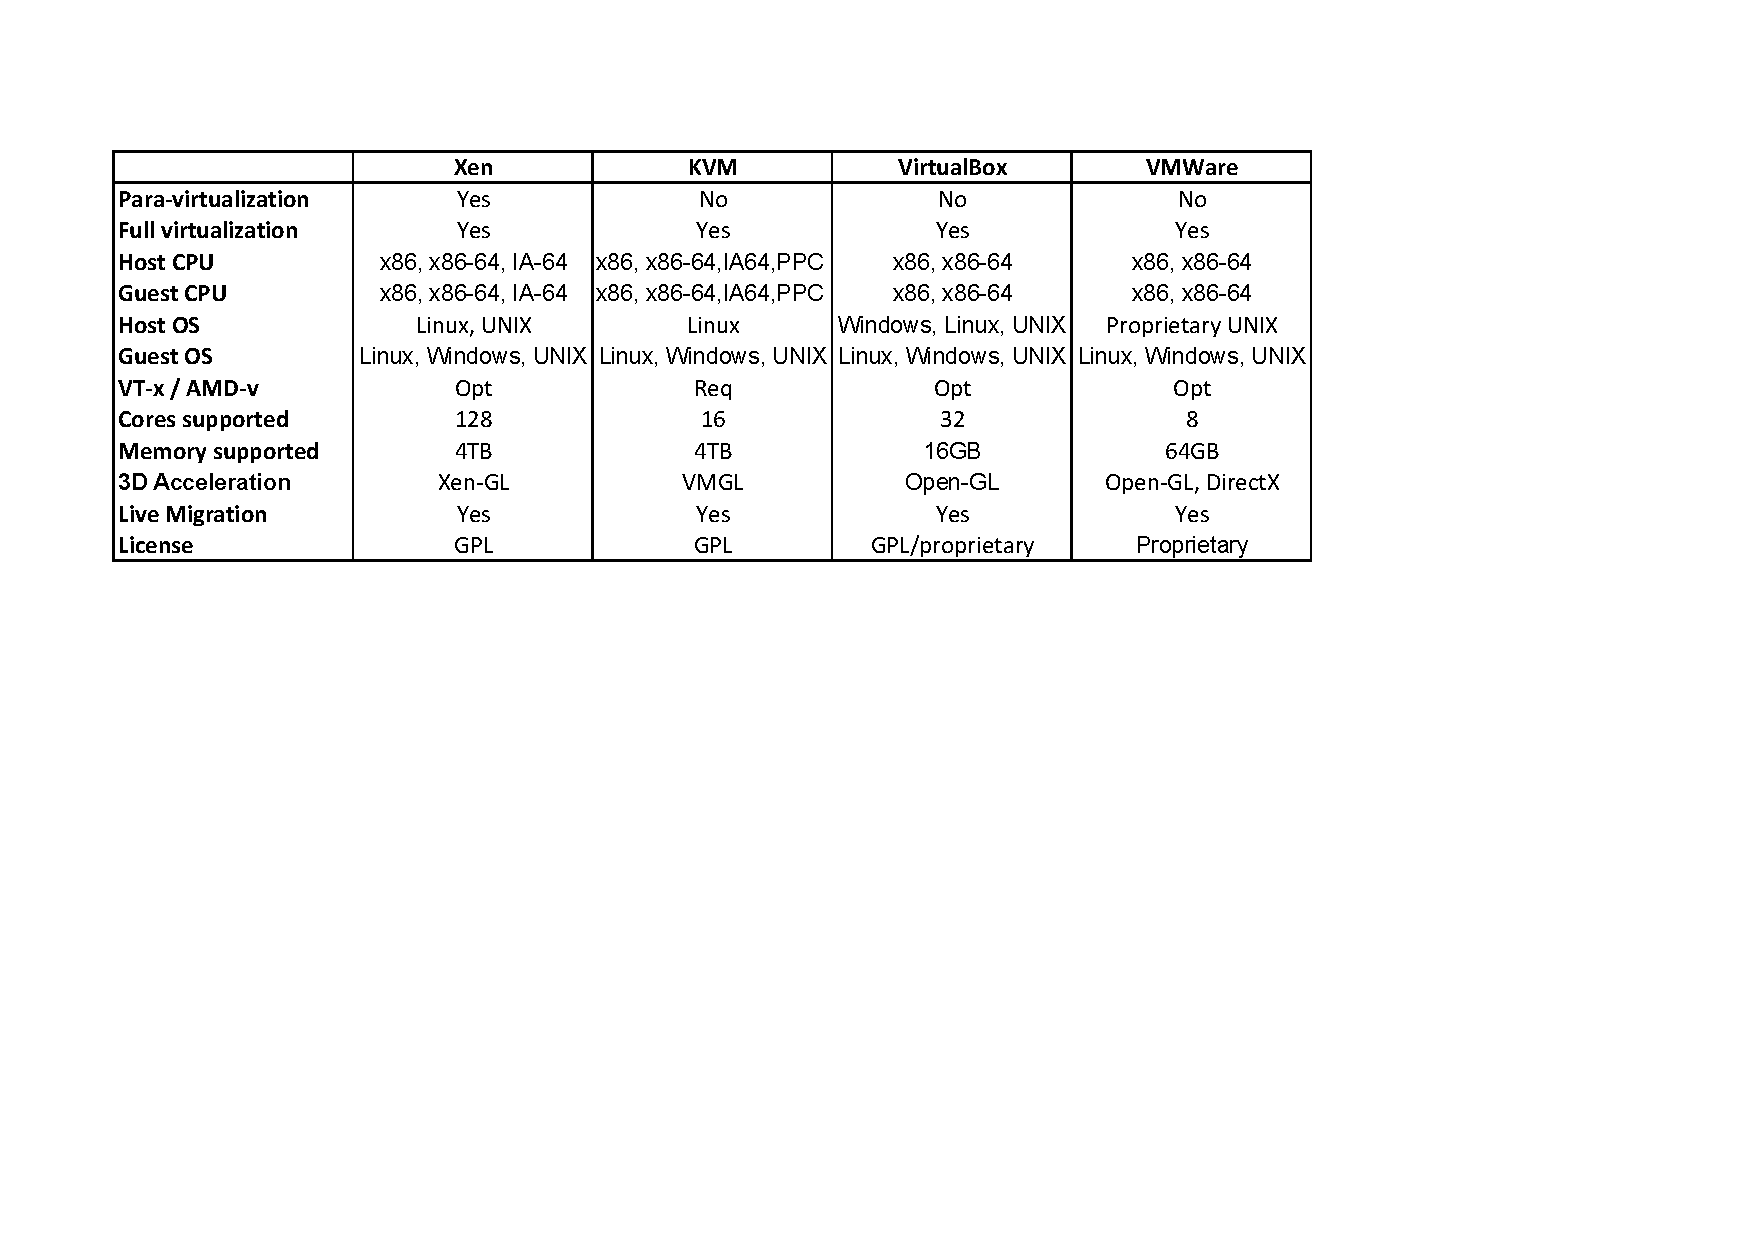
\epsfig{file=images/virt-comparison.pdf,  width=6in}
%\caption{A comparison chart between Xen, KVM, VirtualBox, and VMWare ESX} 
%\end{figure*} 


The first point of investigation is the virtualization method of each VM.  Each hypervisor supports full virtualization, which is now common  practice within most x86 virtualization deployments today.  Xen, originating as a para-virtualized VMM, still supports both types, however full virtualization is often preferred as it does not require the manipulation of the guest kernel in any way.  From the Host and Guest CPU lists, we see that x86 and, more specifically, x86-64/amd64 guests are all universally supported.  Xen and KVM both suport Itanium-64 architectures for full virtualization (due to both hypervisors dependency on QEMU), and KVM also claims support for some recent PowerPC architectures. However, we concern ourselves only with x86-64 features and performance, as other architectures are out of the scope of this manuscript.  Of the x86-64 platforms, KVM is the only hypervisor to require either Intel VT-X or AMD-V instruction sets in order to operate.  VirtualBox and VMWare have internal mechanisms to provide full virtualization even without the virtualization instruction sets, and Xen can default back to para-virtualized guests.  

Next, we consider the host environments for each system.  As Linux is the primary OS type of choice within HPC deployments, its key that all hypervisors support Linux as a guest OS, and also as a host OS. As VMWare ESX is meant to be a virtualization-only platform, it is built upon a specially configured Linux/UNIX proprietary OS specific to its needs.  All other hypervisors support Linux as a host OS, with VirtualBox also supporting Windows, as it was traditionally targeted for desktop-based virtualization.  However, as each hypervisor uses VT-X or AMD-V instructions, each can support any modern OS targeted for x86 platforms, including all variants of Linux, Windows, and UNIX. 

While most hypervisors have desirable host and guest OS support, hardware support within a guest environment varies drastically.  Within the HPC environment, virtual CPU (vCPU) and maximum VM memory are critical aspects to choosing the right virtualization technology.  In this case, Xen is the first choice as it supports up to 128 vCPUs and can address 4TB of main memory in 64-bit modes, more than any other.  VirtualBox, on the other hand, supports only 32 vCPUs and 16GB of addressable RAM per guest OS, which may lead to problems when looking to deploy it on large multicore systems.  KVM also faces an issue with the number of vCPU supported limited to 16, recent reports indicate it is only a soft limit \cite{Harper2009}, so deploying KVM in an SMP environment may not be a significant hurdle. Furthermore, all hypervisors provide some 3D acceleration support (at least for OpenGL) and support live migration across homogeneous nodes, each with varying levels of success.  

Another vital juxtaposition of these virtualization technologies is the license agreements for its applicability within HPC deployments.  Xen, KVM, and VirtualBox are provided for free under the GNU Public License (GPL) version 2, so they are open to use and modification by anyone within the community, a key feature for many potential users.  While VirtualBox is  under GPL, it has recently also offered with additional features under a more proprietary license dictated by Oracle since its acquirement from Sun last year.  VMWare, on the other hand, is completely proprietary with an extremely limited licensing scheme that even prevents the authors from willfully publishing any performance benchmark data without specific and prior approval.  As such, we have neglected VMWare form the remainder of this manuscript. Whether going with a proprietary or open source hypervisor, support can be acquired (usually for an additional cost) with ease from each option.   

\subsection{Usability}

While side by side feature comparison may provide crucial information about a potential user's choice of hypervisor, that may also be interested in its ease of installation and use.  We will take a look at each hypervisor from two user perspectives, a systems administrator and normal VM user.  

One of the first things on any system administrator's mind on choosing a hypervisor is the installation.  For all of these hypervisors, installation is relatively painless.  For the FutureGrid support group, KVM and VirualBox are the easiest of the all tested hypervisors to install, as there are a number of supported packages available and installation only requires the addition of one or more kernel modules and the support software.  Xen, while still supported in binary form by many Linux distributions, is actually much more complicated.  This is because Xen requires a full modification to the kernel itself, not just a module.  Loading a new kernel into the boot process which may complicate patching and updating later in the system's maintenance cycle.  VMWare ESX, on the other hand, is entirely separate from most other installations.  As previously noted, ESX is actually a hypervisor and custom UNIX host OS combined, so installation of ESX is likewise to installing any other OS from scratch.  This may be either desirable or adverse, depending on the system administrator's usage of the systems and VMWare's ability to provide a secure and patched environment.

While system administrators may be concerned with installation and maintenance, VM users and Cloud developers are more concerned with daily usage. The first thing to note about all of such virtualiation technologies is they are supported (to some extent) by the libvirt API \cite{Bolte2010}.  Libvirt is commonly used by many of today's IaaS Cloud offerings, including Nimbus, Eucalyptus, OpenNebula and OpenStack.  As such, the choice of hypervisor for Cloud developer's is less of an issue, so long as the hypervisor supports the features they desire.  For individual command line usage of each tool, it varies quite a bit more.  Xen does provide their own set of tools for controlling and monitoring guests, and seem to work relatively well but do incur a slight learning curve.  KVM also provides its own CLI interface, and while it is often considered less cumbersome it provides less advanced features directly to users, such as power management or quick memory adjustment (however this is subject to personal opinion).  One advantage of KVM is each guest actually runs as a separate process within the host OS, making it easy for a user to manage and control the VM inside the host if KVM misbehaves.  VirtualBox, on the other hand, provides the best command line and graphical user interface.  The CLI, is especially well featured when compared to Xen and KVM as it provides clear, decisive and well documented commands, something most HPC users and system administrators alike will appreciate.  VMWare provides a significantly enhanced GUI as well as a Web-based ActiveX client interface that allows users to easily operate the VMWare host remotely.  In summary, there is a wide variance of interfaces provided by each hypervisor, however we recommend Cloud developers to utilize the libvirt API whenever possible.  


%%%%%%%%%%%%%%%%%%%%%%%%%%%%%%%%%%%%%%%%%%%%%%%%%%%%%%%%%%%%%%%%%%%%%%
\section{Experimental Design}
%%%%%%%%%%%%%%%%%%%%%%%%%%%%%%%%%%%%%%%%%%%%%%%%%%%%%%%%%%%%%%%%%%%%%%

In order to provide an unaltered and unbiased review of these virtualization technologies for Clouds, we need to outline a neutral testing environment.  To make this possible, we have chosen to use FutureGrid as our virtualization and cloud test-bed.  


\subsection{The FutureGrid Project}

FutureGrid (FG) \cite{www-fg} provides computing capabilities that enable researchers to tackle complex research challenges related to the use and security of Grids and Clouds. These include topics ranging from authentication, authorization, scheduling, virtualization, middleware design, interface design and cybersecurity, to the optimization of Grid-enabled and cloud-enabled computational schemes for researchers in astronomy, chemistry, biology, engineering, atmospheric science and epidemiology. 

The test-bed includes a geographically distributed set of heterogeneous computing systems, a data management system that will hold both metadata and a growing library of software images necessary for Cloud computing, and a dedicated network allowing isolated, secure experiments, as seen in Figure \ref{F:3}. The test-bed supports virtual machine-based environments, as well as operating systems on native hardware for experiments aimed at minimizing overhead and maximizing performance. The project partners are integrating existing open-source software packages to create an easy-to-use software environment that supports the instantiation, execution and recording of grid and cloud computing experiments.


 \FIGURE{htb}
  {images/FG-map.pdf}
  {1.0}
  {FutureGrid Participants and Resources}
  {F:3}


One of the goals of the project is to understand the behavior and utility of Cloud computing approaches.  However, it is not clear at this time which of these toolkits will become the users' choice toolkit. FG provides the ability to compare these frameworks with each other while considering real scientific applications \cite{las2010gce}. Hence, researchers are be able to measure the overhead of cloud technology by requesting linked experiments on both virtual and bare-metal systems, providing valuable information that help decide which infrastructure suits their needs and also helps users that want to transition from one environment to the other.  These interests and research objectives make the FutureGrid project the perfect match for this work.  Furthermore, we expect that the results gleaned from this manuscript will have a direct impact on the FutureGrid deployment itself.  

\subsection{Experimental Environment}

Currently, one of FutureGrid's latest resources is the {\it India} system, a 256 CPU IBM iDataPlex machine consisting of 1024 cores, 2048 GB of ram, and 335 TB of storage within the Indiana University Data Center.  In specific, each compute node of India has two Intel Xeon 5570 quad core CPUs running at 2.93Ghz, 24GBs of Ram, and a QDR InfiniBand connection.  A total of four nodes were allocated directly from India for these experiments.  All were loaded with a fresh installation of Red Hat Enterprise Linux server 5.5 x86\_64 with the 2.6.18-194.8.1.el5 kernel patched. Three of the four nodes were installed with different hypervisors; Xen version 3.1, KVM (build 83), and VirtualBox 3.2.10, and the forth node was left as-is to act as a control for bare-metal native performance.  

Each guest virtual machine was also built using Red Hat EL server 5.5 running an unmodified kernel using full virtualization techniques.  All tests were conducted giving the guest VM 8 cores and 16GB of ram to properly span a compute node.  Each benchmark was run a total of 20 times, with the results averaged to produce consistent results, unless indicated otherwise.


\subsection{Benchmarking Setup}

As this manuscript aims to objectively evaluate each virtualization technology from a side-by-side comparison as well as from a performance standpoint, the selection of benchmarking applications is critical.  

The performance comparison of each virtual machine is based on two well known industry standard performance benchmark suites; HPCC and  SPEC. These two benchmark environments are recognized for their standardized reproducible results in the HPC communit, and the National Science Foundation (NSF), Department of Energy (DOE), and DARPA are all sponsors of the HPCC benchmarks. The following benchmarks provide a means to stress and compare processor, memory, inter-process communication, network, and overall performance and throughput of a system.  These benchmarks were selected due to their importance to the HPC community sinse they are often directly correlated with overall application performance \cite{Dujmovic1998}. 
 


\subsubsection{HPCC Benchmarks}
The HPCC Benchmarks \cite{luszczek2006hpc, Dongarra2010} are an industry standard for performing benchmarks for HPC systems. The benchmarks are aimed at testing the system on multiple levels to test their performance. It consists of 7 different tests:

\begin{itemize}
\item {\em HPL} - The Linpack TPP benchmark measures the floating point rate of execution for solving a linear system of equations.  This benchmark is perhaps the most important benchmark within HPC today, as it is the basis of evaluation for the Top 500 list \cite{www-top500}.
 \item {DGEMM} - Measures the floating point rate of execution of double precision real matrix-matrix multiplication.
\item {\em STREAM} - A simple synthetic benchmark program that measures sustainable memory bandwidth (in GB/s) and the corresponding computation rate for simple vector kernel.
\item {\em PTRANS} - Parallel matrix transpose exercises the communications where pairs of processors communicate with each other simultaneously. It is a useful test of the total communications capacity of the network.
\item {\em RandomAccess} - Measures the rate of integer random updates of memory (GUPS).
\item {\em FFT} - Measures the floating point rate of execution of double precision complex one-dimensional Discrete Fourier Transform (DFT).
\item {\em Communication bandwidth and latency} - A set of tests to measure latency and bandwidth of a number of simultaneous communication patterns; based on b\_eff (effective bandwidth benchmark).
\end{itemize}


This benchmark suite uses each test to stress test the performance on multiple aspects of the system. It also provides reproducible results which can be verified by other vendors. This benchmark is used to create the Top 500 list \cite{www-top500} which is the list of the current top supercomputers in the world. The results that are obtained from these benchmarks provide an unbiased performance analysis of the hypervisors. Our results provide insight on inter-node PingPong bandwidth, PingPong latency, and FFT calculation performance. 

\subsubsection{SPEC Benchmarks}

The Standard Performance Evaluation Corporation (SPEC) \cite{dixit1991, www-spec} is the other major standard for evaluation of benchmarking systems. SPEC has several different testing components that can be utilized to benchmark a system. For our benchmarking comparison we will use the SPEC OMP2001 because it appears to represent a vast array of new and emerging parallel applications wile simultaniously providing a comparison to other SPEC benchmarks.  SPEC OMP continues the SPEC tradition of giving HPC users the most objective and representative benchmark suite for measuring the performance of SMP (shared memory multi-processor) systems.

\begin{itemize}

\item The benchmarks are adapted from SPEC CPU2000 and contributions to its search program.
\item The focus is to deliver systems performance to real scientific and engineering applications.
\item The size and runtime reflect the needs of engineers and researchers to model large complex tasks.
\item Two levels of workload characterize the performance of medium and large sized systems.
\item Tools based on the SPEC CPU2000 toolset make these the easiest ever HPC tests to run.
\item These benchmarks place heavy demands on systems and memory.

\end{itemize}



%%%%%%%%%%%%%%%%%%%%%%%%%%%%%%%%%%%%%%%%%%%%%%%%%%%%%%%%%%%%%%%%%%%%%%
\section{Performance Comparison}
%%%%%%%%%%%%%%%%%%%%%%%%%%%%%%%%%%%%%%%%%%%%%%%%%%%%%%%%%%%%%%%%%%%%%%

The goal of this manuscript is to effectively compare and contrast the various virtualization technologies, specifically for supporting HPC-based Clouds.  The first set of results represent the performance of HPCC benchmarks.  Each benchmark was run a total of 20 times, and the mean values taken with error bars represented using the standard deviation over the 20 runs.  The benchmarking suite was built using the Intel 11.1 compiler, uses the Intel MPI and MKL runtime libraries, all set with defaults and no optimizations whatsoever.

We open first with High Performance Linpack (HPL), the de-facto standard for comparing resources.  In Figure \ref{F:hpl}, we can see the comparison of Xen, KVM, and Virtual Box compared to native bare-metal performance.  First, we see that native is capable of around 73.5 Gflops which, with no optimizations, achieves 75\% of the theoretical peak performance.  Xen, KVM and VirtualBox perform at 49.1, 51.8 and 51.3 Gflops, respectively when averaged over 20 runs.  However Xen, unlike KVM and VirtualBox, has a high degree of variance between runs.  This is an interesting phenomenon for two reasons.  First, this may impact performance metrics for other HPC applications and cause errors and delays between even pleasingly-parallel applications and add to reducer function delays.  Second, this wide variance breaks a key component of Cloud computing providing a specific and predefined quality of service.  If performance can sway as widely as what occurred for Linpack, then this may have a negative impact on users.   


 \FIGURE{htb}
  {images/linpack.png}
  {1.0}
  {Linpack performance}
  {F:hpl}


Next, we turn to another key benchmark within the HPC community, Fast Fourier Transforms (FFT).  Unlike the synthetic Linpack benchmark, FFT is a specific, purposeful benchmark which provides results which are often regarded as more relative to a user's real-world application than HPL.  From Figure \ref{F:fft}, we can see rather distinct results from what was previously provided by HPL. Looking at Star and Single FFT, its clear performance across all hypervisors is roughly equal to bare-metal performance, a good indication that HPC applications may be well suited for use on VMs.  The results for MPI FFT also show similar results, with the exception of Xen, which has a decreased performance and high variance as seen in the HPL benchmark.  Our current hypothesis is that there is an adverse affect of using Intel's MPI runtime on Xen, however the investigation is still ongoing.

\FIGURE{htb}
  {images/FFT.png}
  {1.0}
  {Fast Fourier Transform performance}
  {F:fft}


Another useful benchmark illustrative of real-world performance between bare-metal performance and various hypervisors are the ping-pong benchmarks.  These benchmarks measure the bandwidth and latency of passing packets between multiple CPUs.  With this experiment, all ping-pong latencies are kept within a given node, rather than over the network.  This is done to provide further insight into the CPU and memory overhead withing each hypervisor.  From Figure \ref{F:ppb} the intranode bandwidth performance is uncovered, with some interesting distinctions between each hypervisor.  First, Xen performs, on average, close to native speeds, which is promising for the hypervisor.  KVM, on the other hand, shows consistent overhead proportional to native performance across minimum, average, and maximum bandwidth.  VirtualBox, on the other hand, performs well, in fact too well to the point that raises alarm.  While the minimum and average bandwidths are within native performance, the maximum bandwidth reported by VirtualBox is significantly greater than native measurements, with a large variance.  After careful examination, it appears this is due to how VirtualBox assigns its virtual CPUs.  Instead of locking a virtual CPU to a real CPU, a switch may occur which could benefit on the off-chance the two CPU's in communication between a ping-pong test could in fact be the same physical CPU.  The result would mean the ping-pong packet would remain in cache and result in a higher perceived bandwidth than normal.  While this effect may be beneficial for this benchmark, it may only be an illusion towards the real performance gleaned from the VirtualBox hypervisor. 

\FIGURE{htb}
  {images/pingpongbandwidth.png}
  {1.0}
  {Ping Pong bandwidth performance}
  {F:ppb}

The Bandwidth may in fact be important within the ping-ping benchmark, but the latency between each ping-pong is equally useful in understanding the performance impact of each virtualization technology.  From Figure \ref{F:ppl}, we see KVM and VirtualBox have near-native performance; another promising result towards the utility of hypervisors within HPC systems.  Xen, on the other hand, has extremely high latencies, especially at for maximum latencies, which in turn create a high variance within the average latency within the VM's performance.  


\FIGURE{htb}
  {images/pingponglatency.png}
  {1.0}
  {Ping Pong latency performance (lower is better)}
  {F:ppl}



While the HPCC benchmarks provide a comprehensive view for many HPC applications including Linpack and FFT using MPI, performance of intra-node SMP applications using OpenMP is also investigated.  Figure \ref{F:specomp} illustrates SPEC OpenMP performance across the VMs we concentrate on, as well as baseline native performance.  First, we see that the combined performance over all 11 applications executed 20 times yields the native testbed with the best performance at a SPEC score of 34465.  KVM performance comes close with a score of 34384, which is so similar to the native performance that most users will never notice the difference.  Xen and VirtualBox both perform notably slower with scores of 31824 and 31695, respectively, however this is only an 8\% performance drop compared to native speeds. Further results can be found on the SPEC website \cite{spec2011}. 

\FIGURE{htb}
  {images/spec-omp.png}
  {1.0}
  {Spec OpenMP performance}
  {F:specomp}

%%%%%%%%%%%%%%%%%%%%%%%%%%%%%%%%%%%%%%%%%%%%%%%%%%%%%%%%%%%%%%%%%%%%%%
\section{Discussion}
%%%%%%%%%%%%%%%%%%%%%%%%%%%%%%%%%%%%%%%%%%%%%%%%%%%%%%%%%%%%%%%%%%%%%%

The primary goal of this manuscript is to evaluate the viability of virtualization within HPC.  After our analysis, the answer seems to be a resounding "yes."  However, we also hope to select the best virtualization technology for such an HPC environment.  In order to do this, we combine the feature comparison along with the performance results, and evaluate the potential impact within the FutureGrid testbed.    

From a feature standpoint, most of today's virtualization technologies fit the bill for at least small scale deployment, including VMWare.  In short, each support Linux x86\_64 platforms, use VT-X technology for full virtualization, and support live migration.  Due to VMWare's limited and costly licensing, it is immediately out of contention for most HPC deployments.  From a CPU and memory standpoint, Xen seems to provide the best expandability, supporting up to 128 cpus and 4TB of addressable RAM.  So long as KVM's vCPU limit can be extended, it too shows promise as a feature-full virtualization technology.  One of Virtualbox's greatest limitations was the 16GB maximum memory allotment for individual guest VMs, which actually limited us from giving VMs more memory for our performance benchmarks. If this can be fixed and Oracle does not move the product into the proprietary market, VirtualBox may also stand a chance for deployment in HPC environments.  


\FIGURE{htb}
  {images/benchmark-summary.pdf}
  {1.0}
  {Benchmark rating summary (lower is better)}
  {F:summary}


From the benchmark results previously described, the use of hypervisors within HPC-based Cloud deployments is mixed batch.  Figure \ref{F:summary} summarizes the results based on a 1-3 rating, 1 being best and 3 being worst.   While Linpack performance seems to take a significant performance impact across all hypervisors, the more practical FFT benchmarks seem to show little impact, a notably good sign for virtualization as a whole.  The ping-pong bandwidth and latency benchmarks also seem to support this theory, with the exception of Xen, who's performance continually  has wide fluctuations throughout the majority of the benchmarks.  OpenMP performance through the SPEC OMP benchmarking suite also shows promising results for the use of hypervisors in general, with KVM taking a clear lead by almost matching native speeds. 

While Xen is typically regarded as the most widely used hypervisor, especially within academic clouds and grids, it's performance has shown lack considerably when compared to either KVM or VirtualBox.  In particular, Xen's wide and unexplained fluctuations in performance throughout the series of benchmarks suggests that Xen may not be the best choice for building a lasting quality of service infrastructure upon. From Figure \ref{F:summary}, KVM rates the best across all performance benchmarks, making it the optimal choice for {\em general} deployment in an HPC environment.  Furthermore, this work's illustration of the variance in performance among each benchmark and the applicability of each benchmark towards new applications may make possible the ability to preemptively classify applications for accurate prediction towards the ideal virtualized Cloud environment. We hope to further investigate this concept through the use of the FutureGrid experiment management framework at a later date.


In conclusion, it is the authors' projection that KVM is the best overall choice for use within HPC Cloud environments. KVM's feature-rich experience and near-native performance makes it a natural fit for deployment in an environment where usability and performance are paramount.  Within the FutureGrid project specifically, we hope to deploy the KVM hypervisor across our Cloud platforms in the near future, as it offers clear benefits over the current Xen deployment.  Furthermore, we expect these findings to be of great importance to other public and private Cloud deployments, as system utilization, Quality of Service, operating cost, and computational efficiency could all be improved through the careful evaluation of underlying virtualization technologies. 





 
%% Author: Andrew J. Younge
%% PhD Thesis/Project

%$$$$$$$$$$$$$$$$$$$$$$$$$$$$$$$$$$$$$$$$$$$$$$$$$$$$$$$$$$$$$$$$$$$$%
\chapter{Evaluating GPU Passthrough in Xen for High Performance Cloud Computing}
\label{chap:hpgc2014}
%$$$$$$$$$$$$$$$$$$$$$$$$$$$$$$$$$$$$$$$$$$$$$$$$$$$$$$$$$$$$$$$$$$$$%


%\begin{abstract}

%%%%%%%%%%%%%%%%%%%%%%%%%%%%%%%%%%%%%%%%%%%%%%%%%%%%%%%%%%%%%%%%%%%%%%
\section{Abstract}
%%%%%%%%%%%%%%%%%%%%%%%%%%%%%%%%%%%%%%%%%%%%%%%%%%%%%%%%%%%%%%%%%%%%%%


With the advent of virtualization and Infrastructure-as-a-Service (IaaS), the broader scientific computing community is considering the use of clouds for their technical computing needs. This is due to the relative scalability, ease of use, advanced user environment customization abilities clouds provide, as well as many novel computing paradigms available for data-intensive applications. However, there is concern about a performance gap that exists between the performance of IaaS when compared to typical high performance computing (HPC) resources, which could limit the applicability of IaaS for many potential scientific users. 

Most recently, general-purpose graphics processing units (GPGPUs or GPUs) have become commonplace within high performance computing. We look to bridge the gap between supercomputing and clouds by providing GPU-enabled virtual machines (VMs) and investigating their feasibility for advanced scientific computation.  Specifically, the Xen hypervisor is utilized to leverage specialized hardware-assisted I/O virtualization and PCI passthrough in order to provide advanced HPC-centric Nvidia GPUs directly in guest VMs. This methodology is evaluated by measuring the performance of two Nvidia Tesla GPUs within Xen VMs and comparing to bare-metal hardware. Results show PCI passthrough of GPUs within virtual machines is a viable use case for many scientific computing workflows, and could help support high performance cloud infrastructure in the near future.

%\end{abstract}


%\keywords{ High Performance Computing, Cloud Computing, GPU, Virtualization} 

%%%%%%%%%%%%%%%%%%%%%%%%%%%%%%%%%%%%%%%%%%%%%%%%%%%%%%%%%%%%%%%%%%%%%%
\section{Introduction}
%%%%%%%%%%%%%%%%%%%%%%%%%%%%%%%%%%%%%%%%%%%%%%%%%%%%%%%%%%%%%%%%%%%%%%


Cloud computing \cite{aboveTheClouds} has established itself as a prominent paradigm within the realm of Distributed Systems \cite{tanenbaum2002distributed} in a very short period of time. Clouds are an internet-based solution that provide computational and data models for utilizing resources, which can be accessed directly by users on demand in a uniquely scalable way. Cloud computing functions by providing a layer of abstraction on top of base hardware to enable a new set of features that are otherwise intangible or intractable. These benefits and features include Scalability, a guaranteed Quality of Service (QoS), cost effectiveness, and direct user customization via a simplified user interface \cite{wang2010ngc}.



While the origin of cloud computing is based in industry through solutions such as Amazon's EC2 \cite{www-amazon-ec2}, Google's MapReduce \cite{DBLP:journals/cacm/DeanG08}, and Microsoft's Azure \cite{Azure}, the paradigm has since become integrated in all areas of science and technology.  Most notably, there is an increasing effort within the High Performance Computing (HPC) community to leverage the utility of clouds for advanced scientific computing to solve a number of challenges still standing in the field. This can be clearly seen in large-scale efforts such as the FutureGrid project \cite{FG2010design}, the  Magellan project \cite{MagellanFinal}, and through various other Infrastructure-as-a-Service projects including OpenStack \cite{openstack2013},  Nimbus \cite{virtualwork}, and Eucalyptus \cite{EucalyptusPaper}.  


Within HPC, there has also been a notable movement toward dedicated accelerator cards such as general purpose graphical processing units (GPGPUs, or GPUs) to enhance scientific computation problems by upwards of two orders of magnitude. This is accomplished through dedicated programming environments, compilers, and libraries such as CUDA \cite{nvidia2008programming} from Nvidia as well as the OpenCL effort \cite{stone2010opencl}.  When combining GPUs in an otherwise typical HPC environment or supercomputer, major gains in performance and computational ability have been reported in numerous fields \cite{Che2008cuda, Liu08kmeansgpu}, ranging from Astrophysics to Bioinformatics. Furthermore, these gains in computational power have also reportedly come at an increased performance-per-watt \cite{hong2010integrated}, a metric that is increasingly important to the HPC community as we move closer to exascale computing \cite{kogge2008exascale} where power consumption is quickly becoming the primary constraint.


With the advent of both clouds and GPUs within the field of scientific computing, there is an immediate and ever-growing need to provide heterogeneous resources, most immediately GPUs, within a cloud environment in the same scalable, on-demand, and user-centric way that many cloud users are already accustomed to \cite{crago2011heterogeneous}.  While this task alone is nontrivial, it is further complicated by the high demand for performance within HPC.  As such, it is performance that is paramount to the success of deploying GPUs within cloud environments, and thus is the central focus of this work.


The rest of this chapter is organized as follows.  First, in Section 2, we discuss the related research and the options currently available for providing GPUs within a virtualized cloud environment.  In Section 3, we discuss the methodology for providing GPUs directly within virtual machines.  In Section 4 we outline the evaluation of the given methodology using two different Nvidia Tesla GPUs and compare to the best-case native application in Section 5. Then, we discuss the implications of these results in Section 6 and consider the applicability of each method within a production cloud system.  Finally, we conclude with our findings and suggest directions for future work.


%%%%%%%%%%%%%%%%%%%%%%%%%%%%%%%%%%%%%%%%%%%%%%%%%%%%%%%%%%%%%%%%%%%%%%
\section{Virtual GPU Directions}
%%%%%%%%%%%%%%%%%%%%%%%%%%%%%%%%%%%%%%%%%%%%%%%%%%%%%%%%%%%%%%%%%%%%%%

Recently, GPU programming has been a primary focus for numerous scientific computing applications. Significant progress has been accomplished in many different workloads, both in science and engineering, based on parallel abilities of GPUs for floating point operations and very high on-GPU memory bandwidth. This hardware, coupled with CUDA and OpenCL programming frameworks, has led to an explosion of new GPU-specific applications. In some cases,  GPUs outperform even the fastest multicore counterparts by an order of magnitude \cite{sanders2010cuda}.  In addition, further research could leverage the per-node performance of GPU accelerators with the high speed, low latency interconnects commonly utilized in supercomputers and clusters  to create a hybrid GPU + MPI class of applications. The number of distributed GPU applications is increasing substantially in supercomputing, usually scaling many GPUs simultaneously \cite{kindratenko2009gpu}. 

Since the establishment of cloud computing in industry, research groups have been evaluating its applicability to science \cite{foster2008cca}. Historically, HPC and Grids have been on similar but distinct paths within distributed systems, and have concentrated on performance, scalability, and solving complex, tightly coupled problems within science. This has led to the development of supercomputers with many thousands of cores, high speed, low latency interconnects, and sometimes also coprocessors and FPGAs \cite{barker2008entering, craven2007examining}.  Only recently have these systems been evaluated from a cloud perspective \cite{MagellanFinal}.  An overarching goal exists to provide HPC Infrastructure as its own service (HPCaaS) \cite{shainer2009scheduling}, aiming to classify and limit the overhead of virtualization, and reducing the bottlenecks classically found in CPU, memory, and  I/O operations within hypervisors \cite{Younge2011cloud, jackson2010performance}. Furthermore, the transition from HPC to cloud computing becomes more complicated when we consider adding GPUs to the equation.


GPU availability within a cloud is a new concept that has sparked a large amount of interest within the community.  The first successfully deployment of GPUs within a cloud environment was the Amazon EC2 GPU offering.  A collaboration between Nvidia and Citrix also exists to provide cloud-based gaming solutions to users using the new Kepler GPU architecture \cite{www-nvidiacitrix}. However, this is currently not targeted towards HPC applications. 

The task of providing a GPU accelerator for use in a virtualized cloud environment is one that presents a myriad of challenges.  This is due to the complicated nature of virtualizing drivers, libraries, and the heterogeneous offerings of GPUs from multiple vendors. Currently, two possible techniques exist to fill the gap in providing GPUs in a cloud infrastructure: back-end I/O virtualization, which this chapter focuses on, and Front-end remote API invocation.

\subsection{Front-end Remote API invocation}

One method for using GPUs within a virtualized cloud environment is through front-end library abstractions, the most common of which is remote API invocation.  Also known as API remoting or API interception, it represents a technique where API calls are intercepted and forwarded to a remote host where the actual computation occurs.  The results are then returned to the front-end process that spawned the invocation, potentially within a virtual machine.  The goal of this method is to provide an emulated device library where the actual computation is offloaded to another resource on a local network. 

Front-end remote APIs for GPUs have been implemented by a number of different technologies for different uses. To solve the problem of graphics processing in VMs, VMWare \cite{vmwaregpu} has developed a device-emulation approach that emulates the Direct3D and OpenGL calls to leverage the host OS graphics processing capabilities to provide a 3D environment within a VM. API interception through the use of wrapper binaries has also been implemented by technologies such as Chromium \cite{humphreys2002chromium}, and Blink. However these graphics processing front-end solutions are not suitable for general purpose scientific computing, as they do not expose interfaces that CUDA or OpenCL can use. 

Currently, efforts are being made to provide a front-end remote API invocation solutions for the CUDA programming architecture.  vCUDA \cite{shi2012vcuda} was the first of such technologies to enable transparent access of GPUs within VMs by API call interception and redirection of the CUDA API. vCUDA substitutes the CUDA runtime library and supports a transmission mode using XMLRPC, as well as a sharing mode that is built on VMRPC, a dedicated remote procedure call architecture for VMM platforms. This share model can leads to better performance, especially as the volume of data increases, although there may be limitations in VMM interoperability. 

Like vCUDA, gVirtuS uses API interception to enable transparent CUDA, OpenCL, and OpenGL support for Xen, KVM, and VMWare virtual machines~\cite{gvirtus}.  gVirtuS uses a front-end/back-end model to provide a VMM-independent abstraction layer to GPUs.  Data transport from gVirtuS' front-end to the back-end is accomplished through a combination of shared memory, sockets, or other hypervisor-specific APIs.  gVirtuS' primary disadvantage is in its decreased performance in host-to-device and device-to-host data movement due to overhead of data copies to and from its shared memory buffers. Recent work has also enabled the dynamic sharing of GPUs by leveraging the gVirtus back-end system with relatively good results \cite{gCloud}, however process-level GPU resource sharing is outside the scope of this manuscript.


rCUDA \cite{duato2010rcuda, duato2011enabling}, a recent popular remote CUDA framework, also provides remote API invocation to enable VMs to access remote GPU hardware by using a sockets based implementation for high-speed near-native performance of CUDA based applications. rCUDA recently added support for using InfiniBand's high speed, low latency network to increase performance for CUDA applications with large data volume requirements. rCUDA version 4.1 also supports the CUDA runtime API version 5.0, which supports peer device memory access and unified addressing. One drawback of this method is that rCUDA cannot implement the undocumented and hidden functions within the runtime framework, and therefore does not support all CUDA C extensions.  While rCUDA provides some support tools, native execution of CUDA programs is not possible and programs need to be recompiled or rewritten to use rCUDA. Furthermore, like gVirtuS and many other solutions, performance between host-to-device data movement is only as fast as the underlying interconnect, and in the best case with native RDMA InfiniBand, is roughly half as fast as native PCI Express usage when using the standard QDR InfiniBand.



\begin{comment}
%%%%%%%%%%%%%%%%%%%%%%%%%%%%%%%%%%%%%%%%%%%%%%%%%%%%%%%%%%%%%%%%%%%%%%
\section{Design and Implementation} 
%%%%%%%%%%%%%%%%%%%%%%%%%%%%%%%%%%%%%%%%%%%%%%%%%%%%%%%%%%%%%%%%%%%%%%
\end{comment}

\subsection{Back-end PCI passthrough}

Another approach to using a GPU in a virtualized environment is to provide a VM with direct access to the GPU itself, instead of relying on a remote API. This chapter focuses on such an approach.  Devices on a host's PCI-express bus are virtualized using directed I/O virtualization technologies recently implemented by chip manufacturers, and then direct access is relinquished upon request to a guest VM. This can be accomplished using the VT-d and IOMMU instruction sets from Intel and AMD, respectively. This mechanism, typically called PCI passthrough, uses a memory management unit (MMU) to handle direct memory access (DMA) coordination and interrupt remapping directly to the guest VM, thus bypassing the host entirely.  With host involvement being nearly non-existent, near-native performance of the PCI device within the guest VM can be achieved, which is an important characteristic for using a GPU within a cloud infrastructure.

PCI passthrough itself has recently become a standard technique for many other I/O systems such as storage or network controllers.  However, GPUs (even from the same vendor) have additional legacy VGA compatibility issues and non-standard low-level interface DMA interactions that make direct PCI passthrough nontrivial. VMWare has started use of a vDGA system for hardware GPU utilization, however it remains in tech preview and only documentation for Windows VMs is present \cite{vmwaregpu}.  In our experimentation, we have found that the Xen hypervisor provides a good platform for performing PCI passthrough of GPU devices to VMs due to its open nature, extensive support, and high degree of reconfigurability. Work with Xen in \cite{yang2012using} gives hints at good performance for PCI passthrough in Xen, however further evaluation with independent benchmarks is needed when looking at scientific computing with GPUs.

Today's GPUs can provide a variety of frameworks for application programmers to use. Two common solutions are CUDA and OpenCL. CUDA, or the Compute Unified Device Architecture, is a framework for creating and running parallel applications on Nvidia GPUs. OpenCL provides a more generic and open framework for parallel computation on CPUs and GPUs, and is available for a number of Nvidia, AMD, and Intel GPUs and CPUs. While OpenCL provides a more robust and portable solution, many HPC applications utilize the CUDA framework. As such, we focus only on Nvidia based CUDA-capable GPUs as they offer the best support for a wide array of programs, although this work is not strictly limited to Nvidia GPUs.

\section{Implementation}

In this chapter we use a specific host environment to enable PCI passthrough. First, we start with the Xen 4.2.2 hypervisor on Centos 6.4 and a custom 3.4.50-8 Linux kernel with Dom0 Xen support.  Within the Xen hypervisor, GPU devices are seized upon boot and assigned to the xen-pciback kernel module. This process blocks the host devices form loading the Nvidia or nouveau drivers, keeping the GPUs uninitialized and therefore able to be assigned to DomU VMs.  

Xen, like other hypervisors, provides a standard method of passing through PCI devices to guest VMs upon creation.  When assigning a GPU to a new VM, Xen loads a specific VGA BIOS to properly initialize the device enabling DMA and interrupts to be assigned to the guest VM. Xen also relinquishes control of the GPU via the xen-pciback module. From there, the Linux Nvidia drivers are loaded and the device is able to be used as expected within the guest. Upon VM termination, the xen-pciback module re-seizes the GPU and the devices can be re-assigned to new VMs in the future. 

\FIGURE{!htb}
  {images/pci-passthrough-gpu}
  {1.0}
  {GPU PCI passthrough within the Xen Hypervisor}
  {F:passthrough}

This mechanism of PCI passthrough for GPUs can be implemented using multiple devices per host, as illustrated in Figure \ref{F:passthrough}. Here, we see how the device's connection to the VM totally bypasses the Dom0 host as well as the Xen VMM, and is managed by  VT-d or IOMMU to access the PCI-Express bus which the GPUs utilize. This is in contrast to other common virtual device uses, where hardware is emulated by the host and shared across all guests. This is the common usage for Ethernet controllers and input devices to enable users to interact with VMs as they would with native hosts, unlike the bridged model shown in the figure.  The potential downside of this method is there can be a 1:1 or 1:N mapping of VMs to GPUs only. A M:1 mapping where multiple VMs use a GPU is not possible.  However, almost all scientific applications environments using GPUs generally do not share GPUs between processes or other nodes, as doing so would cause unpredictable and serious performance degradation. As such, this GPU isolation within a VM can be considered an advantage in many contexts.

\subsection{Feature Comparison}

Using the GPU PCI passthrough technique described previously has a number of advantages compared to front-end API implementations. First, it allows for an operating environment that more closely relates to native bare-metal usage of GPUs. Essentially, a VM provides a nearly identical infrastructure to clusters and supercomputers with integrated GPUs. This lowers the learning curve for many researchers, and even enables researchers to potentially use other tools within a VM that might not be supported within a supercomputer or cluster.  Unlike with remote API implementations, users don't need to recompile or modify their code, as the GPUs are essentially local to the data. Further comparing to remote API implementations, using PCI passthrough within a VM allows users to leverage any GPU framework available, OpenCL or CUDA, and any higher level programming frameworks such as within Matlab or Python.

Through the use of advanced scheduling techniques within cloud infrastructure, we can also take advantage of PCI passthrough implementation for efficiency purposes. Users could request VMs with GPUs which get scheduled for creation on machines that provide such resources, but can also request normal VMs as well.  The scheduler can correctly map VM requirement requests to heterogeneous hardware. This enables large scale resources to support a wide array of scientific computing applications without the added cost of putting GPUs in all compute nodes.


%%%%%%%%%%%%%%%%%%%%%%%%%%%%%%%%%%%%%%%%%%%%%%%%%%%%%%%%%%%%%%%%%%%%%%
\section{Experimental Setup} 
%%%%%%%%%%%%%%%%%%%%%%%%%%%%%%%%%%%%%%%%%%%%%%%%%%%%%%%%%%%%%%%%%%%%%%


In this chapter back-end GPU PCI passthrough to virtual machines using the Xen hypervisor is detailed, however proper evaluation of the performance of such method needs to be properly considered. As such, we ran an array of benchmarks that evaluate the performance of this method compared to the same hardware running native bare-metal GPU code without any virtualization. We focus our tests on single-node performance to best understand low level overhead.


To evaluate the effectiveness of GPU-enabled VMs within Xen, two different machines were used to represent two generations of Nvidia GPUs. The first system at Indiana University consists of dual-socket Intel Xeon X5660 6-core CPUs at 2.8Ghz with 192GB DDR3 RAM, 8TB RAID5 array, and two Nvidia Tesla "Fermi" C2075 GPUs. The system at USC/ISI uses a dual-socket Intel Xeon E5-2670 8-core CPUs at 2.6Ghz with 48GB DDR3 RAM, 3 600GB SAS disk drives, but with the latest Nvidia Tesla  "Kepler" K20m GPU supplied by Nvidia.  These machines represent the present Fermi series GPUs along with the recently release Kepler series GPUs, providing a well-rounded experimental environment. Native systems were installed with standard Centos 6.4 with a stock 2.6.32-279 Linux kernel. Xen host systems were still loaded with Centos 6.4 but with a custom 3.4.53-8 Linux kernel and Xen 4.2.22.  Guest VMs were also Centos 6.4 with N-1 processors and 24GB of memory and 1 GPU passed through in HVM full virtualization mode. Using both IU and USC/ISI machine configurations in native and VM modes represent the 4 test cases for our work.


In order to evaluate the performance, the SHOC Benchmark suite \cite{danalis2010scalable} was used to extensively evaluate performance across each test platform. The SHOC benchmarks were chosen because they provide a higher level of evaluation regarding GPU performance than the sample applications provided in the Nvidia SDK, and can also evaluate OpenCL performance in similar detail. The benchmarks were compiled using the NVCC compiler in CUDA5 driver and library, along with OpenMPI 1.4.2 and GCC 4.4. Each benchmark was run a total of 20 times, with the results given as an average of all runs. 


%%%%%%%%%%%%%%%%%%%%%%%%%%%%%%%%%%%%%%%%%%%%%%%%%%%%%%%%%%%%%%%%%%%%%%
  \section{Results}
%%%%%%%%%%%%%%%%%%%%%%%%%%%%%%%%%%%%%%%%%%%%%%%%%%%%%%%%%%%%%%%%%%%%%%

Results of all benchmarks are compressed into three subsections: floating point operations, device bandwidth and pci bus performance. Each represents a different level of evaluation for GPU-enabled VMs compared to bare-metal native GPU usage.

\subsection{Floating Point Performance}

Flops, or floating point operations per second, are a common measure of computational performance, especially within scientific computing. The Top 500 list \cite{www-top500} has been the relative gold standard for evaluating supercomputing performance for more than two decades. With the advent of GPUs in some of the fastest supercomputers today, including GPUs identical to those used in our experimentation, understanding the performance relative to this metric is imperative.

Figure \ref{F:shocflops} shows the raw peak FLOPs available using each GPU in both native and virtualized modes. First, we observe the advantage of using the Kepler series GPUs over Fermi, with peak single precision speeds tripling in each case. Even for double precision FLOPs, there is roughly a doubling of performance with the new GPUs. However its most interesting that there is less than a 1\% overhead when using GPU VMs compared to native case for pure floating point operations. The K20m-enabled VM was able to provide over 3 Teraflops, a notable computational feat for any single node.

\FIGURE{!htb}
  {images/xen-gpu-figs/flops}
  {1.0}
  {GPU Floating Point Operations per Second}
  {F:shocflops} 

Figures \ref{F:shocfft} and \ref{F:shocmm} show Fast Fourier Transform (FFT) and the Matrix Multiplication implementations across both test platforms. For all benchmarks that do not take into account the PCI-Express (pcie) bus transfer time, we again see near-native performance using the Kepler GPUs and Fermi GPUs when compared to bare metal cases. Interestingly, overhead within Xen VMs is consistently less than 1\%, confirming the synthetic MaxFlops benchmark above.  However, we do see some performance impact when calculating the total FLOPs with the pcie bus in the equation. This performance decrease ranges significantly for the C2075-series GPU,  roughly about a 15\% impact for FFT and a 5\% impact for Matrix Multiplication.  This overhead in pcie runs is not as pronounced for the Kepler K20m test environment, with near-native performance in all cases (less than 1\%).  


%With PCIE included in the overall performance card differences decrase because the PCI-Express bus 2.0 is limited to 8GT/s, which both cards use blahblah

\FIGURE{!htb}
  {images/xen-gpu-figs/fft}
  {1.0}
  {GPU Fast Fourier Transform}
  {F:shocfft} 

\FIGURE{!htb}
  {images/xen-gpu-figs/mm}
  {1.0}
  {GPU Matrix Multiplication}
  {F:shocmm} 


Other FLOP-based benchmarks are used to emulate higher level applications.  Stencil represents a 9-point stencil operation applied to a 2D data set, and the S3D benchmark is a computationally-intensive kernel from the S3D turbulent combustion simulation program \cite{hawkes2005direct}. In Figure \ref{F:shocs3d}, we see that both the Fermi C2075 and Kepler K20m GPUs performing well compared to the native base case, showing the overhead of virtualization is low.  The C2075-enabled VMs experience slightly more overhead when compared to native performance again for pcie runs, but overhead is at most 7\% for the S3D benchmark. 


\FIGURE{!htb}
  {images/xen-gpu-figs/stencils3d}
  {1.0}
  {GPU Stencil and S3D}
  {F:shocs3d} 



\subsection{Device Speed}

While floating point operations allow for the proposed solution to relate to many traditional HPC applications, they are just one facet of GPU performance within scientific computing. Device speed, measured in both raw bandwidth and additional benchmarks, provides a different perspective towards evaluating GPU PCI passthrough in Xen. Figure \ref{F:shocbw} illustrates device level memory access of various GPU device memory structures. With both Nvidia GPUs, virtualization has little to no impact on the performance of inter-device memory bandwidth. As expected the Kepler K20m outperformed the C2075 VMs and there was a higher variance between runs with both native and VM cases.  Molecular Dynamics and Reduction benchmarks in Figure \ref{F:shocmdred} perform again at near-native performance without the pcie bus taken into account. However the overhead observed increases to 10-15\% when the PCI-Express bus is considered when looking at the Fermi C2075 VMs. 

\FIGURE{!htb}
  {images/xen-gpu-figs/devicememory}
  {1.0}
  {GPU Device Memory Bandwidth}
  {F:shocbw} 


\FIGURE{!htb}
  {images/xen-gpu-figs/mdred}
  {1.0}
  {GPU Molecular Dynamics and Reduction}
  {F:shocmdred} 



\subsection{PCI Express Bus}

Upon evaluating PCI passthrough of GPUs, it is apparent that the PCI express bus is subject to the greatest potential for overhead, as was observed in the Fermi C2075 benchmarks. The VT-d and IOMMU chip instruction sets interface directly with the PCI bus to provide operational and security related mechanisms for each PCI device, thereby ensuring proper function in a multi-guest environment but potentially introducing some overhead. As such, it is imperative to investigate any and all overhead at the PCI Express bus. 

Figure \ref{F:shocbus} looks at maximum PCI bus speeds for each experimental implementation.  First, we see a consistent overhead in the Fermi C2075 VMs, with a 14.6\% performance impact for download (to-device) and a 26.7\% impact in readback (from-device). However, the Kepler K20 VMs do  not experience the same overhead in the PCI-Express bus, and instead perform at near-native performance.  These results indicate that the overhead is minimal in the actual VT-d mechanisms, and instead due to other factors. 




Upon further examination, we have identified the performance degradation within the Fermi-based VM experimental setup is due to the testing environment's NUMA node configuration with the Westmere-based CPUs. With the Fermi nodes, the GPUs are connected through the PCI-Express bus from CPU Socket \#1, yet the experimental GPU VM was run using CPU Socket \#0. This meant that the VM's PCI-Express communication involved more host involvement with Socket \#1, leading to an notable decrease in read and write speeds across the PCI-Express Bus. Such architectural limitations seem to be relieved in the next generation with a Sandy-Bridge CPU architecture and the Kepler K20m experimental setup. In summary, GPU PCI-Express performance in a VM is sensitive to the host CPU's NUMA architecture and care is needed to mitigate the impact, either by leveraging new architectures or by proper usage of Xen's VM core assignment features.  Furthermore, the overhead in this system diminishes significantly when using the new Kepler GPUs by Nvidia.
\FIGURE{!htb}
  {images/xen-gpu-figs/busspeed}
  {1.0}
  {GPU PCI Express Bus Speed}
  {F:shocbus} 



%%%%%%%%%%%%%%%%%%%%%%%%%%%%%%%%%%%%%%%%%%%%%%%%%%%%%%%%%%%%%%%%%%%%%%
\section{Discussion}
%%%%%%%%%%%%%%%%%%%%%%%%%%%%%%%%%%%%%%%%%%%%%%%%%%%%%%%%%%%%%%%%%%%%%%

This chapter evaluates the use of general purpose GPUs within cloud computing infrastructure, primarily targeted towards advanced scientific computing. The method of PCI passthrough of GPUs directly to a guest virtual machine running on a tuned Xen hypervisor shows initial promise for an ubiquitous solution in cloud infrastructure. In evaluating the results in the previous section, a number of points become clear. 

First, we can see that there is a small overhead in using PCI passthrough of GPUs within VMs, compared to native bare-metal usage, which represents the best possible use case. As with all abstraction layers, some overhead is usually inevitable as a necessary trade-off to added feature sets and improved usability. The same is true for GPUs within Xen VMs.  The Kepler K20m GPU-enabled VMs operated at near-native performance for all runs, with a 1.2\% reduction at worst in performance. The Fermi based C2075 VMs experience more overhead due to the NUMA configuration that impacted PCI-Express performance. However, when the overhead of the PCI-Express bus is not considered, the C2075 VMs perform at near-native speeds. % Once improvements in Xen's ability to create CPU pools based on the NUMA architecture are made in order to avoid cross-CPU PCI-Express communication, we expect the performance of the C2075 VMs to increase. 

GPU PCI passthrough also has the potential to perform better than other front-end API solutions that are applicable within VMs, such as gVirtus or rCUDA. This is because such solutions are designed to communicate via a network interconnect such as 10Gb Ethernet or QDR InfiniBand  \cite{rCUDAMellanox}, which introduces an inherent bottleneck. Even with the theoretically optimal configuration of rCUDA using QDR InfiniBand, the maximum theoretical bus speed is 40Gbs, which is comparably less than the measured 54.4Gps real-world performance measured between host-to-device transfers with  GPU-enabled Kepler VMs.  


Overall, it is our hypothesis that the overhead in using GPUs within Xen VMs as described in this chapter will largely go unnoticed by most mid-level scientific computing applications.  This is especially true when using the latest Sandy-Bridge CPUs with the Kepler series GPUs.  We expect many mid-tier scientific computing groups to benefit the most from the ability to use GPUs in a scientific cloud infrastructure. Already this has been confirmed in \cite{jo2013exploiting}, where similar a methodology has been leveraged specifically for Bioinformatics applications in the cloud. 


%%%%%%%%%%%%%%%%%%%%%%%%%%%%%%%%%%%%%%%%%%%%%%%%%%%%%%%%%%%%%%%%%%%%%%
\section{Chapter Summary and Future Work}
%%%%%%%%%%%%%%%%%%%%%%%%%%%%%%%%%%%%%%%%%%%%%%%%%%%%%%%%%%%%%%%%%%%%%%

The ability to use GPUs within virtual machines represents a leap forward for supporting advanced scientific computing within cloud infrastructure. The method of direct PCI passthrough of Nvidia GPUs using the Xen hypervisor offers a clean, reproducible solution that can be implemented within many Infrastructure-as-a-Service (IaaS) deployments. Performance measurements indicate that the overhead of providing a GPU within Xen is minimal compared to the best-case native use, however NUMA inconsistencies can impact performance. The New Kepler-based GPUs operate with a much lower overhead, making those GPUs an ideal choice when designing a new GPU IaaS system. 

Next steps for this work could involve providing GPU-based PCI passthrough within the OpenStack nova IaaS framework. This will enable research laboratories and institutions to create new private or national-scale cloud infrastructure that have the ability to support new scientific computing challenges.  Other hypervisors could also leverage GPU PCI passthrough techniques and warrant in-depth evaluation in the future. Furthermore, we hope to integrate this work with advanced interconnects and other heterogeneous hardware and provide a parallel high performance cloud infrastructure to enable mid-tier scientific computing. 


 
%% Author: Andrew J. Younge
%% PhD Thesis/Project

%$$$$$$$$$$$$$$$$$$$$$$$$$$$$$$$$$$$$$$$$$$$$$$$$$$$$$$$$$$$$$$$$$$$$%
\chapter{GPU-Passthrough Performance: A Comparison of KVM, Xen, VMWare ESXi, and LXC for CUDA and OpenCL Applications}
\label{chap:cloud2014}
%$$$$$$$$$$$$$$$$$$$$$$$$$$$$$$$$$$$$$$$$$$$$$$$$$$$$$$$$$$$$$$$$$$$$%


\begin{comment}
\begin{abstract}
As more scientific workloads are moved into the cloud, the need for high
performance accelerators increases.  Accelerators such as GPUs offer
improvements in both performance and power efficiency over traditional
multi-core processors; however, their use in the cloud has been limited.  Today,
several common hypervisors support GPU-passthrough, but their performance has
not been systematically characterized.  

In this chapter we show that low overhead PCI passthrough is achievable across 4
major hypervisors and two processor microarchitectures. We compare the performance of two generations of NVIDIA
GPUs within the Xen, VMWare ESXi, and KVM hypervisors, and we also compare the
performance to that of Linux Containers (LXC). We show that GPU passthrough to
KVM achieves 98--100\% of the base system's performance across two
architectures, while Xen and VMWare achieve 96--99\% of the base systems
performance, respectively.   In addition, we describe several
valuable lessons learned through our analysis and share the
advantages and disadvantages of each hypervisor/PCI passthrough solution. 

\end{abstract}
\end{comment}
\section{Introduction}
%Proposed contribution 
%\begin{enumerate} \item Demonstrate GPU Passthrough performance across 4
%standard hypervisors (what's the best word for this, given that LXC isn't
%really a hypervisor?) \item Any others?

%JP will write this, about ~ 3/4 of a page

%\end{enumerate}

% Add something that describes the necessity to use GPUs/Accellerators in "Cloud"

As scientific workloads continue to demand increasing performance at greater
power efficiency, high performance architectures have been driven towards heterogeneity and
specialization.  Intel's Xeon Phi, and GPUs from both NVIDIA and AMD represent some
of the most common accelerators, with each capable of delivering improved
performance and power efficiency over commodity multi-core CPUs. 


%Yet today's
%Infrastructure-as-a-Service (IaaS) clouds are largely homogeneous, with little
%or no access to accelerators.  


 Infrastructure-as-a-Service (IaaS) clouds have the potential to
democratize access to the latest, fastest, and most powerful computational
accelerators.  This is true of both public and private clouds.  Yet today's
clouds are typically homogeneous without access to even the most commonly used
accelerators.  Historically, enabling virtual machine access to GPUs and other PCIe devices has
proven complex and error-prone, with only a small subset of GPUs being
certified for use within a few commercial hypervisors.  This is especially true
for NVIDIA GPUs, likely the most popular for scientific computing, but whose
drivers have always been closed source.  

Given the complexity surrounding the choice of GPUs, host systems, and
hypervisors, it is perhaps no surprise that Amazon is the only major cloud
provider offering customers access to GPU-enabled instances.  All of this is
starting to change, however, as open source and other freely available
hypervisors now provide sufficiently robust PCI passthrough functionality to
enable GPU and other accelerator access whether in the public or private cloud.

Today, it is possible to access GPUs at high performance within all of
the major hypervisors, merging many of the advantages of cloud computing (e.g. custom
images, software defined networking, etc.)  with
the accessibility of on-demand accelerator hardware.  Yet, no study to date has
systematically compared the performance of PCI passthrough across all major
cloud hypervisors.  Instead, alternative solutions have been proposed that
attempt to virtualize the GPU~\cite{Duato2010rc}
, but sacrifice performance.

%Instead, alternative solutions have been proposed that attempt to virtualize the
%GPU~\cite{Duato2010rcuda, shi2012vcuda, Gupta:2009, giunta2010gvirtus}. These solutions, typically based on library
%interposition, essentially redirect the CUDA, OpenCL, OpenGL, or DirectX library calls in order
%to access GPUs via a network or other shared memory device.  This approach works
%well for some workloads, including desktop virtualization, but is insufficient for performance
%critical code.  

In this chapter, we characterize the performance of both NVIDIA Fermi and Kepler GPUs
operating in PCI passthrough mode in VMWare VSphere, Linux KVM, Xen, and Linux
Containers (LXC).  Through a series of microbenchmarks as well as scientific and
Big Data applications, we make two contributions: 

\begin{enumerate}
\item We demonstrate that PCI passthrough at high performance is possible for
GPUs across 4 major hypervisors.
\item We describe the lessons learned through our performance analysis, as well as the relative advantages
and disadvantages of each hypervisor for GPU support.
\end{enumerate}

%In this paper we characterize the performance of the NVIDIA Kepler K20 GPU
%across VMWare VSphere 5.5, KVM, Xen, and Linux Containers (LXC).  Through a
%series of microbenchmarks as well as common scientific and Big Data
%applications, we make the following contributions: 

%\begin{enumerate} 

%\item[1.] Demonstrate GPU passthrough performance across 4 major hypervisors.  

%\item[2.] Describe the lessons learned through our PCI passthrough hypervisor
%analysis.

%\end{enumerate}

%The remainder of this paper is organized as follows: in
%Section~\ref{BACKGROUND}, we describe PCI passthrough within the context of
%%both GPUs and general PCI devices; in Section~\ref{RELATED}, we describe the
%prior work in the area of virtual machine access to GPUs; in
%Section~\ref{METHOD} we present our experimental methodology, benchmarks, and
%system characteristics; in Section~\ref{RESULTS} we characterize each
%hypervisor using both microbenchmarks and real applications; in
%Section~\ref{ANALYSIS} we analyze and discuss the results; 


%\section{Background}\label{BACKGROUND}
%about 1 page.  JP will coordinate, may get some background from Andrew.

\begin{comment}
\subsection{PCI Passthrough}

Input/Output Memory Management Units, or IOMMUs, play a fundamental roll in the PCI-Passthrough virtualization mechanism. Like traditional MMUs that provide a virtual memory address space to CPUs \cite{Jacob1998}, an IOMMU serves the fundamental purpose of connecting a direct memory access (DMA) capable I/O bus to main memory. The IOMMU unit, typically within the chipset, maps device virtual addresses to physical memory addresses. This process also has the added improvement of guaranteeing device isolation by blocking rouge DMA and interrupt requests \cite{yassour2008direct}, with a slight overhead, especially in early implementations \cite{ben2007price}. 

The IOMMU is usually used for providing high performance networking solutions to guest VMs \cite{rixner2008network, dong2008sr, liu2010ipdps} it is also a key component for enabling GPU PCI-Passthrough. As most hypervisors remap guest main memory, and current graphics cards use DMA to read and write between main memory and GPU device memory. Without IOMMU, the PCI device's bus wouldn't be useable within a guest VM. With IOMMU,  DMA remapped is utilized for a given virtual address space within a guest VM, thereby allowing for the PCI device to be used directly within the guest. This also eliminates the need for any resource-intensive emulation or other host involvement after the guest VM is created.

Currently two major IOMMU implementations exist, VT-d \cite{hiremane2007intel, intelvtd} and AMD-Vi\cite{amd2007technology} by Intel and AMD, respecively. Both specifications provide DMA remapping to enable PCI-Passthrough as well as other features such as Interrupt remapping, hypervisor snooping, and security control mechanisms to esnure proper and efficient hardware utilization.  While other IOMMU implementations exist, this manuscript focuses exclusively on VT-d due to our use of two different Intel architectures.  


% I don't think there's much advantage to introducing SR-IOV here as these devices are not using it and its out of the scope

\subsection{GPU Passthrough}

While generic PCI-Passthrough can be used with IOMMU technologies to pass through various PCI-Express devices, GPUs represent a special case which has hampered usage until only recently. In traditional usage, GPUs usually serve as VGA devices primarily to render screen output and while the purposes of scientific computing using GPUs do not require this function, it still exists in legacy. In GPU-Passthrough, another VGA device (such as onboard graphics built into the motherboard) is necessary to serve as the primary display for the host, as well as providing emulated VGA devices for each guest VM. Most GPUs also have a video bios that requires full inititialization and reset functions, which is often difficult due to the proprietary nature of the cards and their drivers. 

There is a wide range of implementation differences of PCI-Passthrough between the hypervisors studies in this manuscript. However, type 1 and 2 hypervisors such as KVM, Xen, and VMWare all operate on similar principals. LXC, a linux container solution, does not use traditional PCI-Passthrough of GPUs, as described later.  For hypervisors, the IOMMU must first be built into the kernel and enabled within the kernel bootloader parameters. This allows DMA and interrupt mechanisms to be properly initialized before any devices are initialized. Next, the original device's drivers must be blacklisted, either within the kernel or directly as a module to ensure the PCI device (in our case the GPU) is not initialized by the host. Later in the boot order, a hypervisor specific module will sieze the device to prevent any furter initialization or tampering, while also making the device visible to the host. In KVM, this is accomplished with the new vgio driver to seize a GPU whenb booting. Xen uses the pci-back driver and VMWare leverages their VMDirectPath I/O mechanism for similar results. During guest VM creation, the hypervisor will relinquish control of the PCI device and the device will be passed through to the guest. Finally, the VM can load standard drivers and use the device as expected, in our case for scientific computing problems.


\end{comment}



\section{Related Work \& Background}\label{RELATED}

GPU virtualization and GPU-passthrough are used within a variety of contexts,
from high performance computing to virtual desktop infrastructure.  Accessing one or
more GPUs within a virtual machine is typically accomplished by one of two
strategies: 1) via API remoting with device emulation; or 2) using PCI
passthrough.  


\subsection {GPU API Remoting}

rCUDA, vCUDA, GViM, and gVirtuS are well-known API
remoting solutions%~\cite{Duato2010rcuda, shi2012vcuda, Gupta:2009, giunta2010gvirtus}.
Fundamentally, these approaches operate similarly by splitting the driver into a
front-end/back-end model, where calls into the interposed CUDA library
(front-end)  are sent via shared memory or a network interface to the back-end
service that executes the CUDA call on behalf of the virtual machine.  Notably,
this technique is not limited to CUDA, but can be used to decouple OpenCL,
OpenGL, and other APIs from their local GPU or accelerator. 

%The general purpose of GPU virtualization is to centralize management and administration by utilizing overall hardware resources and improving scalability~\cite{Yang2012}. We can categorize virtualization into  two types according to the defined virtualization boundary between the stack and physical GPU hardware. One is to run the graphics driver in the host/hypervisor such as API Remoting and device emulation, and the other is to run the graphic driver stack inside the Virtual Machine (VM) such as pass-through technique~\cite{Dowty2009, Yang:2012}.

%NVIDIA's Compute Unified Device Architecture (CUDA) is a parallel computing platform and scalable parallel programming model~\cite{Yang2012, Yang:2012, Song:2013}. For the virtualization of the CUDA Runtime API for VMs, several virtualization approaches are available, such as rCUDA, vCUDA, GPU-accelerated Virtual Machines(GViM) and gVirtuS~\cite{Yang:2012, Gupta:2009}. rCUDA employs Sockets API to let the client and server have communication with each other. As a General Purpose Graphics Processing Unit (GPGPU) computing solution, vCUDA lets applications in VMs access graphics hardware. GViM virtualizes the graphics accelerator at the level of abstraction, leverages the CUDA APIs and their open source counterparts, and offers low overheads and direct access to accelerator resources by guest OS. gVirtuS is an hypervisor-independent GPU Virtualization Service. Also, as a new approach to GPU resource management, Gdev integrates runtime support into the OS by adopting more appropriate scheduling algorithm for compute-intensive workload~\cite{Kato:2012}. 

The performance of API-remoting depends largely on the application and the
remoting solution's implentation.  Bandwidth
and latency-sensitive benchmarks and applications will tend to expose performance bottlenecks
more than compute-intensive applications.  Moreover, solutions
that rely on high speed networks, such as Infiniband, will compete with
application-level networking for bandwidth.  


\subsection{PCI Passthrough}

Input/Output Memory Management Units, or IOMMUs, play a fundamental roll in the
PCI-passthrough virtualization mechanism. Like traditional MMUs that provide a
virtual memory address space to CPUs \cite{Jacob1998}, an IOMMU serves the
fundamental purpose of connecting a direct memory access (DMA) capable I/O bus
to main memory. The IOMMU unit, typically within the chipset, maps device
virtual addresses to physical memory addresses. This process also has the added
improvement of guaranteeing device isolation by blocking rogue DMA and interrupt requests \cite{yassour2008direct}, with a slight overhead, especially in early implementations \cite{ben2007price}. 

%The IOMMU is usually used for providing high performance networking solutions
%to guest VMs \cite{rixner2008network, dong2008sr, liu2010ipdps} it is also a
%key component for enabling GPU PCI-passthrough. As most hypervisors remap guest main memory, and current graphics cards use DMA to read and write between main memory and GPU device memory. Without IOMMU, the PCI device's bus wouldn't be useable within a guest VM. With IOMMU,  DMA remapped is utilized for a given virtual address space within a guest VM, thereby allowing for the PCI device to be used directly within the guest. This also eliminates the need for any resource-intensive emulation or other host involvement after the guest VM is created.

Currently two major IOMMU implementations exist, \mbox{VT-d}  and
{AMD-Vi} by Intel and AMD, respectively. Both
specifications provide DMA remapping to enable PCI-passthrough as well as other
features such as interrupt remapping, hypervisor snooping, and security control
mechanisms to ensure proper and efficient hardware utilization. PCI passthrough has been studied within the context of networking~\cite{liu2010ipdps}, storage~\cite{jujjuri2010virtfs}, and other PCI-attached devices; however, GPUs have historically lagged behind other devices in their support for virtual
machine passthrough.  


% I don't think there's much advantage to introducing SR-IOV here as these devices are not using it and its out of the scope

\subsection{GPU Passthrough, a Special Case of PCI Passthrough}

While generic PCI passthrough can be used with IOMMU technologies to pass
through many PCI-Express devices, GPUs represent a special case of PCI
devices, and a special case of PCI passthrough. In traditional usage, GPUs usually serve as VGA devices primarily to
render screen output, and while the GPUs used in this study do not render screen
out, the function still exists in legacy. In GPU-passthrough, another VGA device
(such as onboard graphics built into the motherboard, or a baseboard management
controller) is necessary to serve as the primary display for the host, as well
as providing emulated VGA devices for each guest VM. Most GPUs also have a video
BIOS that requires full initialization and reset functions, which is often difficult due to the proprietary nature of the cards and their drivers. 

%There is a wide range of implementation differences of PCI-passthrough between
%the hypervisors studies in this manuscript. However, type 1 and 2 hypervisors
%such as KVM, Xen, and VMWare all operate on similar principals. LXC, a linux
%container solution, does not use traditional PCI-passthrough of GPUs, as described later.  For hypervisors, the IOMMU must first be built into the kernel and enabled within the kernel bootloader parameters. This allows DMA and interrupt mechanisms to be properly initialized before any devices are initialized. Next, the original device's drivers must be blacklisted, either within the kernel or directly as a module to ensure the PCI device (in our case the GPU) is not initialized by the host. Later in the boot order, a hypervisor specific module will sieze the device to prevent any furter initialization or tampering, while also making the device visible to the host. In KVM, this is accomplished with the new vgio driver to seize a GPU whenb booting. Xen uses the pci-back driver and VMWare leverages their VMDirectPath I/O mechanism for similar results. During guest VM creation, the hypervisor will relinquish control of the PCI device and the device will be passed through to the guest. Finally, the VM can load standard drivers and use the device as expected, in our case for scientific computing problems.


Nevertheless, for applications that require native or near-native GPU performance across the
full spectrum of applications with immediate access to the latest GPU drivers
and compilers, GPU passthrough solutions are preferrable to API remoting.  Today, Citrix Xenserver, open source Xen \cite{Yang:2012}, and VMWare ESXi ~\cite{Dowty2009}, and most recently KVM all support GPU passthrough.  To our knowledge, no one has systematically characterized the performance of GPU passthrough across a range of hypervisors, across such a breadth of benchmarks, and across multiple GPU generations as we do.  

%To our knowledge, this work is the first that describes the use of NVIDIA Tesla GPUs specifically with the KVM hypervisor. % as vfio functionality necessary was only recently introduced in the 3.9 Linux kernel. 



%To cope with I/O performance degradation, Virtual Machine Monitor (VMM)-bypass I/O technologies, including PCI passthrough and SR-IOV, have been introduced~\cite{Nakada:2012}. Device pass-through allows guest operating system to have exclusive access~\cite{Yang:2012}. PCI Express (PCIe) Single-root I/O Virtualization (SR-IOV) works by assigning directly hardware resource of I/O devices to a VM to reduce I/O performance degradation~\cite{Suzuki:2010}. To make migration and checkpoint/restart possible over VMM-bypass I/O devices, Symbiotic Virtualization (SymVirt) is proposed, without the virtualization overhead during normal operations~\cite{Nakada:2012}. And GPUDirect RDMA (GDR) is a feature introduced in CUDA with collaboration of NVIDIA and Mellanox for InifiniBand clusters, that allows third party devices like network adapters to directly access data in GPU device memory, over the PCIe bus~\cite{Potluri:2013}.

%The performance of a virtualized GPU depends on the characteristics of the application under test~\cite{Dowty2009}. API Remoting or device emulation causes significant performance degradation relative to native hardware. But, device pass-through technique can achieve near-native performance and GPU feature set, and maintain driver easily~\cite{Yang:2012}. The inner communication in VM is not through the real hardware but just in the memory on the real machine~\cite{Yang2012}. Also, power-performance efficiency model is proposed at exascale by identifying bottlenecks of power-performance and their main causes on GPU-based heterogeneous HPC systems~\cite{Song:2013}.


\section{Experimental Methodology}\label{METHOD}
%In this paper, we are comparing the performance of a standard CentOS 6.4 virtual
%against a comparable CentOS 6.4 bare metal machine.  However, each hypervisor
%has its own system requirements which


\subsection{Host and Hypervisor Configuration}

We used two hardware systems, named Bespin and Delta, to evaluate four
hypervisors.
The Bespin system at USC/ISI represents Intel's Sandy Bridge microarchitecture with a Kepler class K20 GPU. The Delta system, provided by the FutureGrid project \cite{www-futuregrid}, represents the Westmere microarchitecture with a Fermi class C2075 GPU. 
%  Bespin and Delta are representative of
%Intel's Sandy Bridge and Westmere microarchitectures, respectively.  The Bespin
%system includes a Kepler class K20 GPU, while the Delta system includes a Fermi
%class C2075 GPU.  The Delta system was available as part of the FutureGrid project
Table~\ref{HOSTS} provides
the major hardware characteristics of both systems.  Note that in addition, both
systems include 10 gigabit Ethernet, gigabit Ethernet, and either FDR or QDR
Infiniband. Our experiments do not emphasize networking, and we use the gigabit
ethernet network for management only.


\begin{table}
\small
\renewcommand{\arraystretch}{1.3}
\caption{Host hardware configurations}
\label{HOSTS}
\centering
\begin{tabular}{|l||l|l|}
\hline
 & Bespin & Delta  \\ \hline
CPU (cores)  & 2x E5-2670 (16)  & 2x X5660 (12) \\ \hline
Clock Speed & 2.6 GHz & 2.6 GHz \\ \hline 
RAM &  48 GB &  192 GB \\ \hline
NUMA Nodes & 2 & 2 \\ \hline
GPU &  1x K20m &  2x C2075 \\ \hline

\end{tabular}
\end{table}

A major design goal of these experiments was to reduce or eliminate NUMA effects
(non-uniform memory access) on the PCI passthrough results in order to
facilitate fair comparisons across hypervisors and to reduce experimental noise.  To this end, we
configured our virtual machines and containers to execute only on the NUMA node
containing the GPU under test.  We acknowledge that the NUMA effects on
virtualization may be interesting in their own right, but they are not the
subject of this set of experiments.

We use Bespin and Delta to evaluate three hypervisors and one container-based
approach to GPU passthrough. The hypervisors and container system, VMWare ESXi,
Xen, KVM, and LXC, are summarized in Table~\ref{HYPERVISORS}.  Note that each
virtualization solution imposes its own unique requirements on the base
operating system.  Hence, Xen's Linux kernel refers to the Domain-0 kernel,
whereas KVM's Linux kernel represents the actual running kernel hosting the KVM
hypervisor.  Linux Containers share a single kernel between the host
and guests, and VMWare ESXi does not rely on a Linux kernel at all.  

Similarly, hypervisor requirements prevented us from standardizing on a single host operating system.  For Xen
and KVM, we relied on the Arch Linux 2013.10.01 distribution because it provides
easy access to the mainline Linux kernel.  For our LXC tests, we use CentOS
6.4 because its shared kernel was identical to the base CentOS 6.4 kernel used
in our testing.  VMWare has a
proprietary software stack.  All of this makes comparison challenging, but as we describe in
Section~\ref{GUESTS}, we are running a common virtual machine across all
experiments.

%Our base host system is composed of 2x 8-core Intel Xeon E5-2670 CPUs and 48
%GB of RAM split into two NUMA nodes of one CPU socket and 24 GB RAM.  A single
%NVIDIA Kepler K20m GPU available, and is attached to NUMA node 0.  In addition,
%the node is equipped with 10 Gb Ethernet, FDR Infniband, and gigabit Ethernet.
%All benchmarking is contained within a single node, so neither the 10 Gb
%Ethernet adapter or the FDR Infiniband adapter were used.  The gigabit Ethernet
%adapter was used only as a management network for guest access.

%For our experiments, we compare VMWare ESXi 5.5.0, KVM from Linux Kernel 3.12
%with QEMU version 1.7, Xen 4.3.0 with Linux kernel 3.12 Dom0, and LXC containers based on
%2.6.32-358.23.2 from CentOS 6.4   Both KVM and Xen use an Arch Linux 2013.10.01
%installation as their base distribution.  VMWare ESXi is a proprietary
%bare-metal software stack and is not based on Linux.


%In Table~\ref{HYPERVISORS} we describe the system configuration for each
%hypervisor.  Note that the column Linux Kernel describes the

\begin{table}
\small
\renewcommand{\arraystretch}{1.3}
\caption{Host Hypervisor/Container Configuration}
\label{HYPERVISORS}
\centering
\begin{tabular}{|l||l|l|}
\hline
Hypervisor & Linux Kernel & Linux Version \\ \hline 
KVM & 3.12 & Arch 2013.10.01 \\ \hline 
Xen 4.3.0-7 & 3.12 & Arch 2013.10.01 \\ \hline
VMWare ESXi 5.5.0 & N/A & N/A \\ \hline
LXC & 2.6.32-358.23.2 & CentOS 6.4 \\ \hline

\end{tabular}
\end{table}


%We treat each hypervisor as its own system, comparing a VM composed of CentOS
%6.4 with a bare metal machine running CentOS 6.4. This results in challenges
%when comparing one hypervisor to another 



\subsection{Guest Configuration}\label{GUESTS}

We treat each hypervisor as its own system, and compare virtual machine guests
to a base CentOS 6.4 system. The base system and the guests are all composed of
CentOS 6.4 installation with a 2.6.32-358.23.2 stock
kernel and CUDA version 5.5. Each guest is allocated 20 GB of RAM and a full CPU
socket (either 6 or 8 CPU cores).  Bespin experiments received 8 cores and Delta
experiments received 6 cores.  VMs were restricted to a single NUMA node.  On
the Bespin system, the K20m GPU was attached to NUMA node 0.  On the Delta
system, the C2075 GPU was attached to NUMA node 1.  Hence VMs ran on NUMA node 0
for the Bespin experiments, and node 1 for the Delta experiments. 



\subsection{Microbenchmarks}

Our experiments are composed of a mix of microbenchmarks and application-level
benchmarks, as well as a combination of CUDA and OpenCL benchmarks.  The SHOC
benchmark suite provides a series of microbenchmarks in both OpenCL and
CUDA~\cite{Danalis:2010}. For this analysis, we focus on the OpenCL benchmarks
in order to exercise multiple programming models.  Benchmarks range from
low-level peak Flops and bandwidth measurements, to kernels and
mini-applications.  


\subsection{Application Benchmarks}
For our application benchmarks, we have chosen the LAMMPS molecular
dynamics simulator~\cite{LAMMPS}, the GPU-LIBSVM~\cite{Athanasopoulos:2011}, and the
LULESH shock hydrodynamics simulator~\cite{LULESH}.  These represent a range of
computational characteristics, from computational physics to big data analytics, and are
representative of GPU-accelerated applications in common use. 

\paragraph {LAMMPS} The Large-scale Atomic/Molecular Parallel Simulator
(LAMMPS), is a parallel molecular
dynamics simulator~\cite{LAMMPS,Plimpton1995} used for production MD simulation
on both CPUs and GPUs~\cite{LAMMPSGPU}.  LAMMPS has two packages for GPU
support, the USER-CUDA and GPU packages.
With the USER-CUDA package, each GPU is used by a single CPU, whereas the GPU
package allows multiple CPUs to take advantage of a single GPU.  There are
performance trade-offs with both approaches, but we chose to use the GPU package
in order to stress the virtual machine by exercising multiple CPUs.  Consistent
with the existing GPU benchmarking approaches, our results are based on the
Rhodopsin protein.

%Atomic LJ fluid has low arithmetic intensity, and small neighbor list. As a result, it shows modest speedup of LAMMPS performance improvements using GPU.
%Gay-Berne has high arithmetic intensity and pairwise force calculation. As a result, it shows upper side of LAMMPS performance improvements using GPU.
%In the case of Rhodopsin, Poisson solver running on CPU takes large percentage of the total time, and shows least speedup using GPU among the three benchmarks.
%We believe that those three benchmarks cover a reasonable range of the characteristis of production applications using both CPU cores and a GPU.
%And our study of virtualization overhead of those benchmarks can give the glimpse of the overehad of virtualization of production applications. 

\paragraph{GPU-LIBSVM} LIBSVM is a popular implementation~\cite{Chang:2011} of
the machine learning classification algorithm support vector machine
(SVM). GPU-accelerated LIBSVM~\cite{Athanasopoulos:2011} enhances LIBSVM by
providing GPU-implementations of the kernel matrix computation portion of the
SVM algorithm for radial basis kernels. For benchmarking purposes we use the
NIPS 2003 feature extraction gisette data set. This data set has a high
dimensional feature space and large number of training instances, and these
qualities are known to be computational intensive to generate SVM models. The
GPU-accelerated SVM implementation shows dramatic improvement over the CPU-only
implementation.


\paragraph{LULESH} Hydrodynamics is widely used to model continuum properties
and interactions in materials when there is an applied
force~\cite{LLNL-TR-490254}. Hydrodynamics applications consume approximately one third
of the runtime of data center resource throughout the U.S. DoD (Department of
Defense). The Livermore Unstructured Lagrange Explicit Shock Hydro (LULESH) was
developed by Lawrence Livermore National Lab as one of five challenge problems in the DARPA UHPC program.
LULESH is widely used as a proxy application in the U.S. DOE (Department of
Energy)  co-design effort for exascale applications~\cite{LULESH}. 


%LULESH 1.0
%includes both Kepler and Fermi GPU models which we use in our benchmarking. 
 

\section{Performance Results}\label{RESULTS}

%note: to keep the table readable in plaintext, be sure to set your textwidth=300 (or so), so that lines don't wrap and get ugly.  This has no effect on the Latex output.
\begin{table*}
%\rowcolors{2}{gray!25}{white}
\footnotesize
\caption{SHOC overheads for Bespin (K20) expressed as geometric means of scaled values within a
level, while maximum overheads are expressed as a percentage.  }
\label{K20MEANS}
\centering
    \begin{tabular}{|l|l|l|l|l|l|l|l|l|}
%\rowcolor{gray!50}
    \hline 
    ~  & \multicolumn{8}{c|}{Bespin (K20)} \\ \hline
    ~  & \multicolumn{2}{c|}{KVM} & \multicolumn{2}{c|}{Xen} & \multicolumn{2}{c|}{LXC} & \multicolumn{2}{c|}{VMWare} \\ \hline 
    ~  & Mean   & Max & Mean & Max & Mean & Max & Mean & Max \\ \hline 
    L0 & 0.999   & 1.57   & 0.997 & 3.34   & 1.00   & 1.77  & 1.00  & 1.90     \\ \hline 
    L1 & 0.998   & 1.23   & 0.998 & 1.39   & 1.00   & 1.47  & 1.00  & 0.975   \\ \hline 
    L2 & 0.998   & 0.48   & 0.995 & 0.846  & 0.999  & 1.90  & 0.999 & 1.20   \\ \hline
    ~  & \multicolumn{8}{c|}{Bespin PCIe-only}  \\ \hline
    ~  & \multicolumn{2}{c|}{KVM} & \multicolumn{2}{c|}{Xen} & \multicolumn{2}{c|}{LXC} & \multicolumn{2}{c|}{VMWare}  \\ \hline 
    ~  & Mean   & Max & Mean & Max & Mean & Max & Mean & Max \\ \hline 
    L0 & 0.997   & 0.317   & 0.999  & 0.143 & 0.995  & 0.981  & 0.995 & 1.01      \\ \hline 
    L1 & 0.998   & 0.683   & 0.997  & 1.39  & 1.00   & 0.928  & 1.01  & 0.975   \\ \hline 
    L2 & 0.998   & 0.478   & 0.996  & 0.846 & 1.00   & 0.247  & 1.01  & 0.133    \\ \hline
    \end{tabular}
\end{table*}

\begin{table*}
%\rowcolors{2}{gray!25}{white}
\footnotesize
\caption{SHOC overheads  for Delta (c2075) expressed as geometric means of scaled values within a
level, while maximum overheads are expressed as a percentage.  }
\label{C2075MEANS}
\centering
    \begin{tabular}{|l|l|l|l|l|l|l|l|l|}
%\rowcolor{gray!50}
    \hline 
    ~  &  \multicolumn{8}{c|}{Delta (C2075)} \\ \hline
    ~  & \multicolumn{2}{c|}{KVM} & \multicolumn{2}{c|}{Xen} & \multicolumn{2}{c|}{LXC} & \multicolumn{2}{c|}{VMWare}  \\ \hline 
    ~  & Mean   & Max & Mean & Max & Mean & Max & Mean & Max \\ \hline 
    L0 & 1.01     & 0.031   & 0.969    & 12.7  & 1.00  & 0.073   & 1.00  & 4.95    \\ \hline 
    L1 & 1.00     & 1.45    & 0.959    & 24.0  & 1.00  & 0.663   & 0.933 & 36.6    \\ \hline 
    L2 & 1.00     & 0.101   & 0.982    & 4.60  & 1.00  & 0.016   & 0.962 & 7.01    \\ \hline
    ~  &  \multicolumn{8}{c|}{Delta PCIe-only} \\ \hline
    ~  & \multicolumn{2}{c|}{KVM} & \multicolumn{2}{c|}{Xen} & \multicolumn{2}{c|}{LXC} & \multicolumn{2}{c|}{VMWare} \\ \hline 
    ~  & Mean   & Max & Mean & Max & Mean & Max & Mean & Max \\ \hline 
    L0 & 1.04     & 0.029   & 0.889    & 12.7  & 1.00  & 0.01  & 0.995  & 4.37    \\ \hline 
    L1 & 1.00     & 1.45    & 0.914    & 20.5  & 0.999 & 0.380 & 0.864  & 36.6    \\ \hline 
    L2 & 1.00     & 0.075   & 0.918    & 4.60  & 1.00  & N/A   & 0.869  & 7.01    \\ \hline
    \end{tabular}
\end{table*}



\begin{comment}
\begin{table*}
%\rowcolors{2}{gray!25}{white}
\footnotesize
\caption{SHOC overheads expressed as geometric means of scaled values within a
level, while maximum overheads are expressed as a percentage.  }
\label{MEANS}
\centering
    \begin{tabular}{|l|l|l|l|l|l|l|l|l|l|l|l|l|l|l|l|l|}
%\rowcolor{gray!50}
    \hline 
    ~  & \multicolumn{8}{c|}{Bespin (K20)} & \multicolumn{8}{c|}{Delta (C2075)} \\ \hline
    ~  & \multicolumn{2}{c|}{KVM} & \multicolumn{2}{c|}{Xen} & \multicolumn{2}{c|}{LXC} & \multicolumn{2}{c|}{VMWare} & \multicolumn{2}{c|}{KVM} & \multicolumn{2}{c|}{Xen} & \multicolumn{2}{c|}{LXC} & \multicolumn{2}{c|}{VMWare} \\ \hline 
    ~  & Mean   & Max & Mean & Max & Mean & Max & Mean & Max & Mean  & Max & Mean & Max & Mean & Max & Mean   & Max \\ \hline 
    L0 & 0.999   & 1.57   & 0.997 & 3.34   & 1.00   & 1.77  & 1.00  & 1.90   & 1.01     & 0.031   & 0.969    & 12.7  & 1.00  & 0.073   & 1.00  & 4.95    \\ \hline 
    L1 & 0.998   & 1.23   & 0.998 & 1.39   & 1.00   & 1.47  & 1.00  & 0.975  & 1.00     & 1.45    & 0.959    & 24.0  & 1.00  & 0.663   & 0.933 & 36.6    \\ \hline 
    L2 & 0.998   & 0.48   & 0.995 & 0.846  & 0.999  & 1.90  & 0.999 & 1.20   & 1.00     & 0.101   & 0.982    & 4.60  & 1.00  & 0.016   & 0.962 & 7.01    \\ \hline
    ~  & \multicolumn{8}{c|}{Bespin PCIe-only} & \multicolumn{8}{c|}{Delta PCIe-only} \\ \hline
    ~  & \multicolumn{2}{c|}{KVM} & \multicolumn{2}{c|}{Xen} & \multicolumn{2}{c|}{LXC} & \multicolumn{2}{c|}{VMWare} & \multicolumn{2}{c|}{KVM} & \multicolumn{2}{c|}{Xen} & \multicolumn{2}{c|}{LXC} & \multicolumn{2}{c|}{VMWare} \\ \hline 
    ~  & Mean   & Max & Mean & Max & Mean & Max & Mean & Max & Mean  & Max & Mean & Max & Mean & Max & Mean   & Max \\ \hline 
    L0 & 0.997   & 0.317   & 0.999  & 0.143 & 0.995  & 0.981  & 0.995 & 1.01  & 1.04     & 0.029   & 0.889    & 12.7  & 1.00  & 0.01  & 0.995  & 4.37    \\ \hline 
    L1 & 0.998   & 0.683   & 0.997  & 1.39  & 1.00   & 0.928  & 1.01  & 0.975 & 1.00     & 1.45    & 0.914    & 20.5  & 0.999 & 0.380 & 0.864  & 36.6    \\ \hline 
    L2 & 0.998   & 0.478   & 0.996  & 0.846 & 1.00   & 0.247  & 1.01  & 0.133 & 1.00     & 0.075   & 0.918    & 4.60  & 1.00  & N/A   & 0.869  & 7.01    \\ \hline
    \end{tabular}
\end{table*}
\end{comment}



We characterize GPGPU performance within virtual machines across two hardware
systems, 4 hypervisors, and 3 application sets.  We begin with the SHOC
benchmark suite before describing the GPU-LIBSVM, LAMMPS, and LULESH results.
All benchmarks are run 20 times and averaged.  Results are scaled with respect
to a base CentOS 6.4 system for both systems.  That is, we compare virtualized
Bespin performance to non-virtualized Bespin performance, and virtualized Delta
performance to non-virtualized Delta performance.  Values less than 1 indicate that the base system
outperformed the virtual machine, while values greater than 1 indicate that the
virtual machine outperformed the base system.  In cases where we present
geometric means across multiple benchmarks, the means are taken over these scaled values, and the semantics
are the same: less than 1 indicates overhead in the hypervisor, greater than 1
indicates a performance increase over the base system.


\subsection{SHOC Benchmark Performance}

%In Table~\ref{shoc_l0}, we provide summary results for the SHOC level 0
%benchmarks. These represent low-level device characteristics, including peak
%FLOPS, bandwidth, etc.  For each hypervisor we list the maximum overhead incurred, as well
%as the geometric mean of the full SHOC level 0 results with respect to the base
%CentOS 6.4 system.

%Overall, each hypervisor performed comparably to the base
%system, on average achieving between 99.7--100\% of the base system's performance, depending on the
%hypervisor. LXC and VMWare achieved near-native performance for the  

SHOC splits its benchmarks into 3 Levels, named Levels 0 through 2.  Level 0
represents device-level characteristics, peak Flop/s, bandwidth, etc.  Level 1
characterizes computational kernels: FFT and matrix multiplication, among others.
Finally, Level 2 includes ``mini-applications,`` in this case an implementation
of the S3D, a computational chemistry application.  

Because the SHOC OpenCL benchmarks report more than 70 individual
microbenchmarks, space does not allow us to show each benchmark individually.
Instead, we start with a broad overview of SHOC's performance across all
benchmarks, hypervisors, and systems.  We then discuss in more detail those
benchmarks that either outperformed or underperformed the Bespin (K20) system by
0.50\% or more. We call these benchmarks outliers. As we will show, those
outlier benchmarks identified on the Bespin system, also tend to exhibit
comparable characteristics on the Delta system as well, but the overhead is
typically higher.

%\begin{figure}[ht!]
%\centering
%\fbox{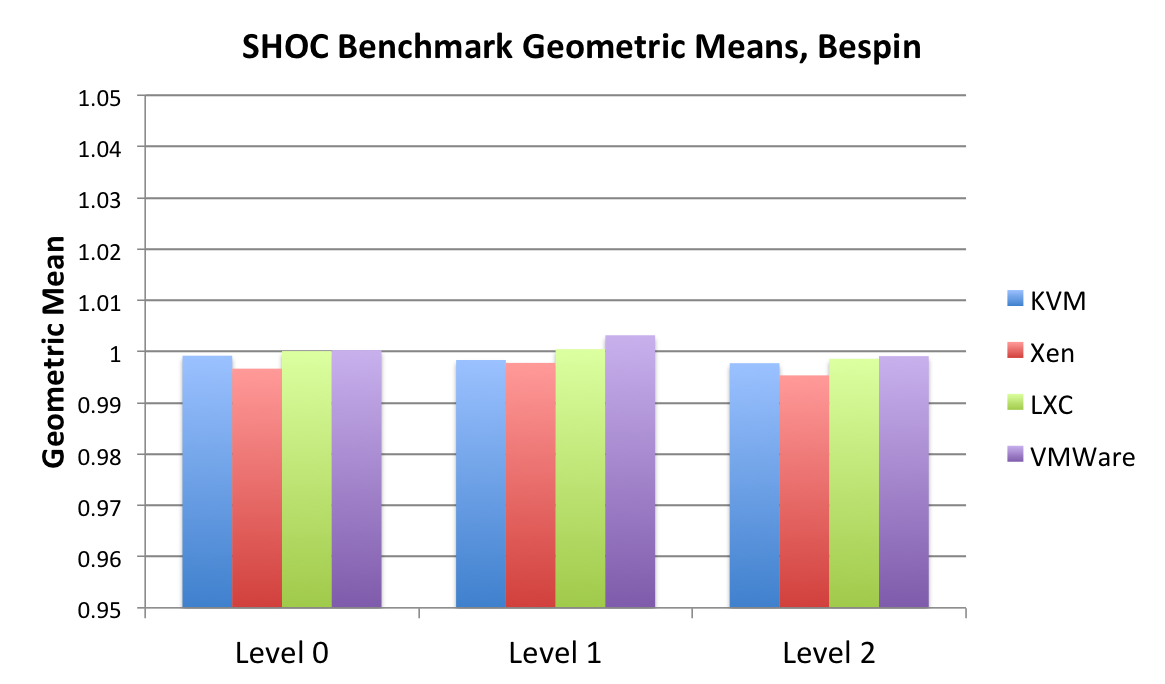
\includegraphics[width=3.25in]{figures/SHOC_means}}
%\caption{SHOC Levels 0-2 geometric means, Bespin hardware.}
%\label{SUMMARY}
%\end{figure}


In Tables~\ref{K20MEANS} and \ref{C2075MEANS}, we provide geometric means for each SHOC level across each
hypervisor and system.  We also include the maximum
overhead for each hypervisor at each level to facilitate comparison across
hypervisors and systems.  Finally, we provide a comparable breakdown of only the
PCIe SHOC benchmarks, based on the intuition that PCIe-specific benchmarks will
likely result in higher overhead.  

At a high level, we immediately notice that in the cases of KVM and LXC, both
perform very near native across both the Bespin and Delta platforms.  On
average, these systems are almost indistinguishable from their non-virtualized
base systems.  So much so, that experimental noise occasionally boosts
performance slightly above their base systems.  

This is in sharp contrast to the Xen and VMWare hypervisors, which perform well
on the Bespin system, but poorly on the Delta system in some cases.  This is
particularly evident when looking at the maximum overheads for Xen and VMWare
across both systems.  In this case, we see that on the Bespin system, Xen's
maximum overhead of 3.34\% is dwarfed by Delta's maximum Xen overhead of 24.0\%.
VMWare exhibits similar characteristics, resulting in a maximum overhead of
1.9\% in the case of the Bespin system, and a surprising 36.6\% in the case of
the Delta system.  We provide a more in-depth discussion of these overheads
below.


\FIGURE{!htb}
  {images/SHOC_L1}
  {1.0}
  {SHOC Levels 0 and 1 relative performance on Bespin system.  Results show benchmarks over or
under-performing by 0.5\% or greater.  Higher is better.}
  {F:SHOC_l1} 

\FIGURE{!htb}
  {images/SHOC_L1-2}
  {1.0}
  {SHOC Levels 1 and 2 relative performance on Bespin system.  Results show benchmarks over or
under-performing by 0.5\% or greater.  Higher is better.}
  {F:SHOC_l1-2} 

\FIGURE{!htb}
  {images/delta-shoc-l0l1}
  {1.0}
  {SHOC Levels 0 and 1 relative performance on Delta system.  Benchmarks
shown are the same as Bespin's.  Higher is better.}
  {F:delta-SHOC_l1} 

\FIGURE{!htb}
  {images/delta-shoc-l1l2}
  {1.0}
  {SHOC Levels 1 and 2 relative performance. Benchmarks shown are the same as
Bespin's.   Higher is better.}
  {F:delta-SHOC_l1-2} 



%\begin{figure}[ht!]
%\centering
%\fbox{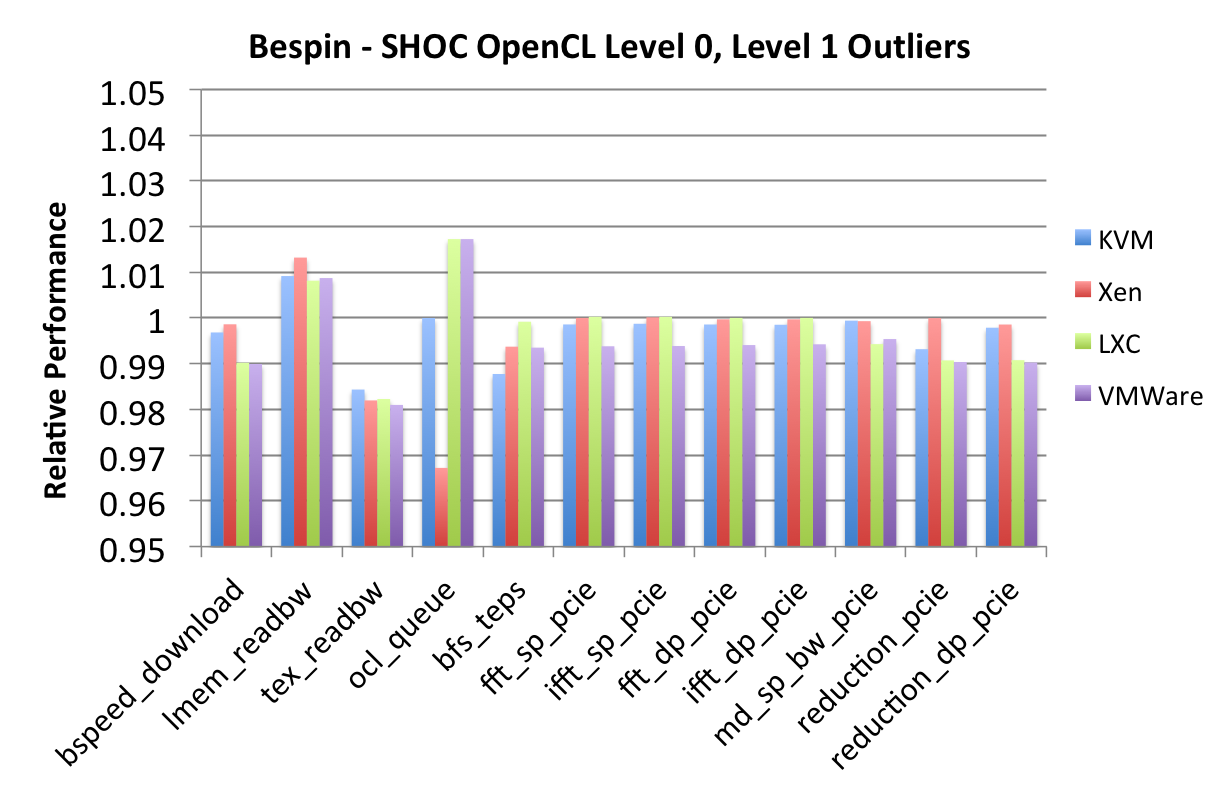
\includegraphics[width=3.25in]{figures/SHOC_L1}}
%\caption{SHOC Levels 0 and 1 relative performance on Bespin system.  Results show benchmarks over or
%under-performing by 0.5\% or greater.  Higher is better.}
%\label{SHOC_l1}
%\end{figure}

%\begin{figure}[ht!]
%\centering
%\fbox{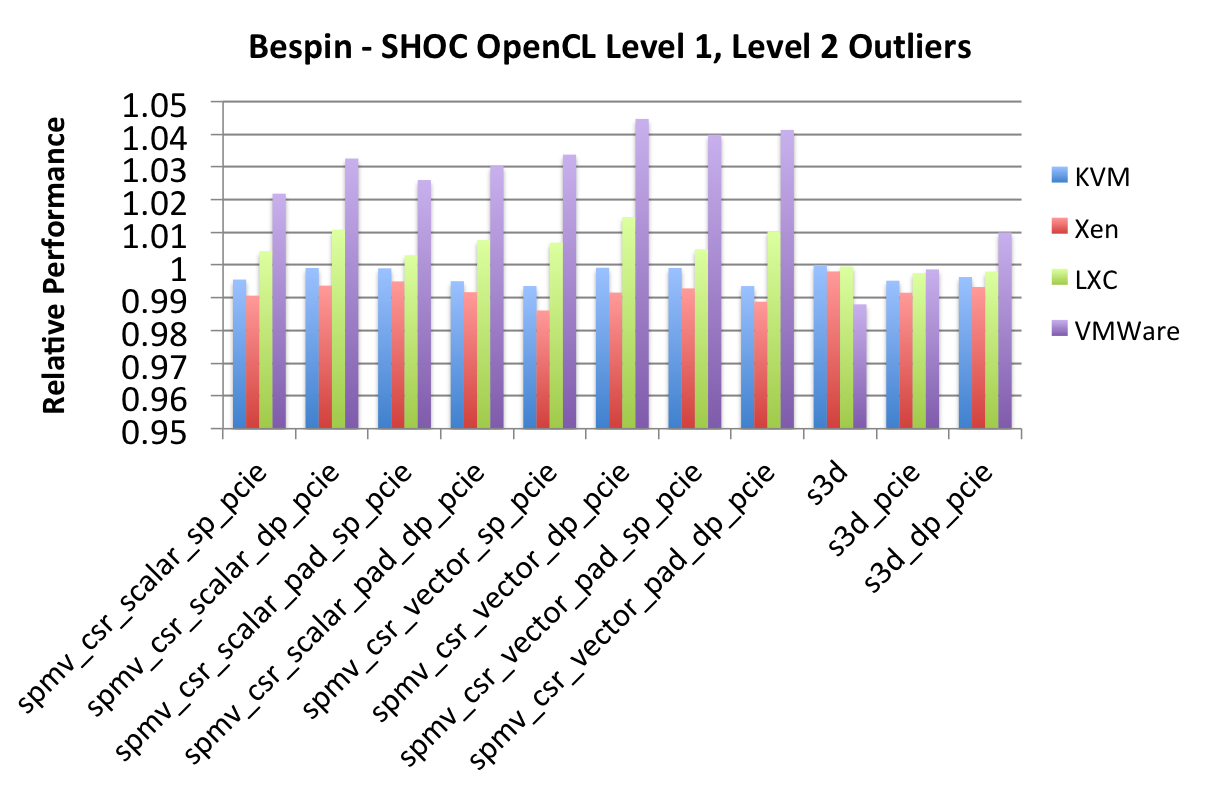
\includegraphics[width=3.25in]{figures/SHOC_L1-2}}
%\caption{SHOC Levels 1 and 2 relative performance on Bespin system.  Results show benchmarks over or
%under-performing by 0.5\% or greater.  Higher is better.}
%\label{SHOC_l1-2}
%\end{figure}

%\begin{figure}[ht!]
%\centering
%\fbox{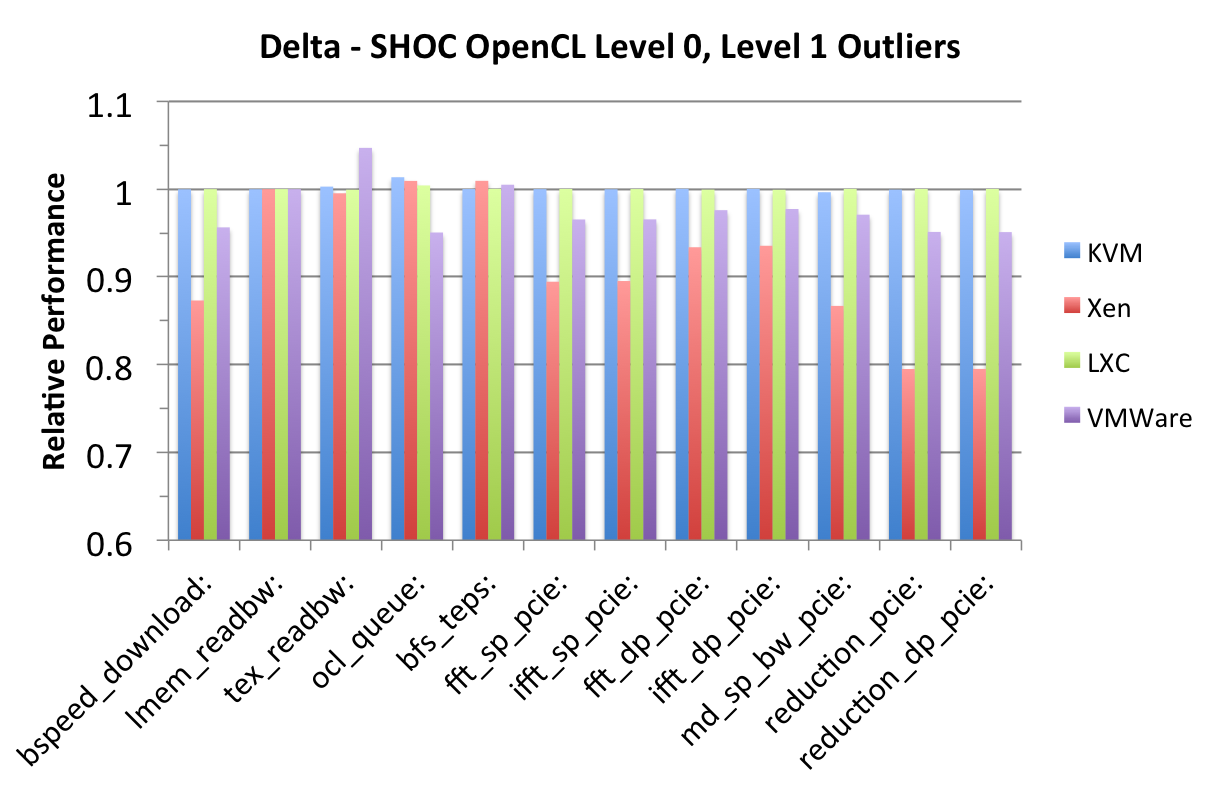
\includegraphics[width=3.25in]{figures/delta-shoc-l0l1.png}}
%\caption{SHOC Levels 0 and 1 relative performance on Delta system.  Benchmarks
%shown are the same as Bespin's.  Higher is better.}
%\label{delta-SHOC_l1}
%\end{figure}

%\begin{figure}[ht!]
%\centering
%\fbox{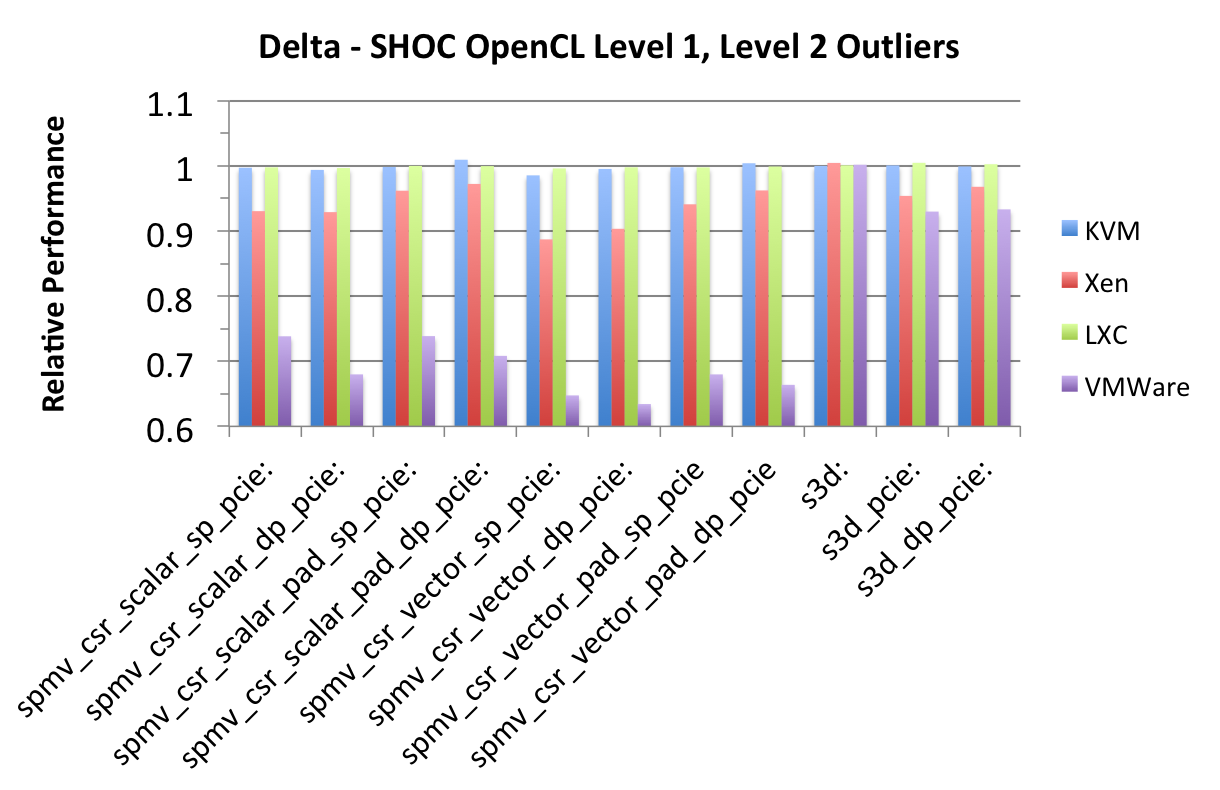
\includegraphics[width=3.25in]{figures/delta-shoc-l1l2.png}}
%\caption{SHOC Levels 1 and 2 relative performance. Benchmarks shown are the same as
%Bespin's.   Higher is better.}
%\label{delta-SHOC_l1-2}
%\end{figure}

%The Bespin
%system, based on a Sandy Bridge CPU with Kepler GPU, averages  99\% efficiency across
%all 4 hypervisors.  Even when considering only the PCIe portion of the SHOC
%benchmarks, virtualization efficiency averages greater than 99\%.   In addition
%to the means, Table~\ref{MEANS} also includes maximum overheads for each SHOC
%level, expressed as a percentage.  In this case we begin to see some slight
%overhead - a maximum of 3.3\% overhead for Xen Level 0 benchmarks, but often
%within 1\% even in the case of the maximum overhead.  

%This contrasts starkly with the Delta system, a Westmere-based Fermi platform,
%which sees overheads as high as 36\% in some cases.  Consequently, the means are
%lowered, particularly in the case of Xen and VMWare for the PCIe-only portion of
%Table~\ref{MEANS}.  Still, KVM and LXC perform very near-native, and under some
%circumstances outpeform the base system.  

%In Figures~\ref{SHOC_l1} and~\ref{SHOC_l1-2} we show the SHOC outlier results
%for the Bespin system.  In Figures~\ref{delta-SHOC_l1} and~\ref{delta-SHOC_l1-2}
%we show the same benchmarks for the Delta system.  We begin the discussion with
%the Bespin system, Figures~\ref{SHOC_l1} and~\ref{SHOC_l1-2}.

Of the Level 0 benchmarks, only four exhibited notable
overhead in the case of the Bespin system: bspeed\_download, lmem\_readbw, tex\_readbw, and ocl\_queue.  These are
shown in Figure~\ref{F:SHOC_l1}.  These benchmarks represent device-level
characteristics, including host-to-device bandwidth, onboard memory reading, and OpenCL
kernel queue delay.  Of the four, only bspeed\_download incurs a statistically
significant overhead.  The remainder perform within one standard deviation of
the base, despite an overhead of greater than 0.5\%.  

bspeed\_download is representative of the most likely source of virtualization overhead, data
movement across the PCI-Express bus.  The PCIe lies at the boundary of
the virtual machine and the physical GPU, and requires interrupt remapping,
IOMMU interaction, etc. in order to enable GPU passthrough into the virtual
machine.  Despite this, in Figure~\ref{F:SHOC_l1} we see a maximum of 1\% overhead
for bspeed\_download in
VMWare, and less than 0.5\% overhead for both KVM and Xen.

The remainder of Figure~\ref{F:SHOC_l1} includes a series of SHOC's Level 1
benchmarks, representing computational kernels.  This includes BFS, FFT, molecular dynamics,
and reduction kernels.  Notably, nearly all of the benchmarks exhibiting
overhead are the PCIe portion of SHOC's benchmarks. This is unsurprising, since
the Level 0 benchmarks suggest PCIe bandwidth as the major source overhead.
Still, results remain consistent with the bspeed\_download overhead observed in
the Level 0 benchmarks, further suggesting that host/device data movement
is the major source of overhead.

In Figure~\ref{F:SHOC_l1-2} we present the remaining SHOC Level 1 results as well
as the SHOC Level 2 results (S3D).  In these results we begin to see an interesting trend,
namely that VMWare consistently outperforms the base system in the Spmv and S3D
microbenchmarks on the Bespin system.  We believe this to be a performance
regression in CentOS 6.4, rather than a unique improvement due to the VMWare ESXi
hypervisor.  When running the benchmarks on a non-virtualized Bespin system with
Arch Linux, the VMWare ESXi performance gains were erased.  An interesting
finding of this was that Spmv was unique in this way - no other benchmarks were
affected by this performance issue.

%We discuss this is more detail in
%Section~\ref{OVERHEADS}.

%We believe this to be a performance regression in
%CentOS 6.4 rather than a unique improvement from VMWare. Executing these
%benchmarks on a non-virtualized Arch Linux system erases VMWare's performance
%gains, suggesting that virtualization, VMWare's Superpages, etc. are not the
%source of the performance improvement.  Nevertheless, we continue to probe the
%performance boost further.

%An interesting characteristic of these benchmarks are that they represent the
%least compute-intensive benchmarks of the entire SHOC suite.  The Spmv
%PCIe benchmarks, for example, perform at less than 1 Gflop/s on both the base
%system as well as the virtual machines.  Because VMWare is the only hypervisor
%to exhibit these characteristics, and because it's closed source, we have
%limited visibility into the low-level performance characteristics.  However, we
%speculate that this may be due to VMWare's very small footprint without even a
%management virtual machine, leaving more resources available to the guest.   

Turning to the Delta system, in Figures~\ref{F:delta-SHOC_l1}
and~\ref{F:delta-SHOC_l1-2}, we show the same benchmarks for the Delta system as
was shown in Figures~\ref{F:SHOC_l1} and~\ref{F:SHOC_l1-2}.  Again, we find that the
same benchmarks are responsible for most of the overhead on the Delta system.  This is
unsurprising, since PCIe was shown to be the source of the bulk of the overhead.
A major difference in the case of the Delta system, however, is the amount of
overhead.  While the Bespin system saw overheads of approximately 1\%, Delta's overhead
routinely jumps above 35\%, especially in the case of the Spmv benchmark for
VMWare.  

On further examination, we determined that Xen was unable to activate
IOMMU large page tables on the Delta system.  KVM successfully allocated 4k, 2M,
and 1G page table sizes, while Xen was limited to size 4k page tables.  The
Bespin system was able to take advantage of 4k, 2M, and 1G page sizes on both
KVM and Xen.  It appears that this issue is correctable and does not represent a
fundamental limitation to the Xen hypervisor on the Nehalem/Westmere
microarchitecture.  While as a closed source product,  we have limited insight
into VMWare ESXi, we speculate that VMWare may be experiencing a similar issue
on the Delta system and not on our Bespin system.

%In Section~\ref{OVERHEADS}, we provide further context for this high

%overhead, but in short, we do not believe this overhead to be a fundamental
%limitation of the Sandy Bridge architecture.  Rather, at least in Xen's case, it
%appears to be a bug in the handling of IOMMU page table sizes.

In light of this, we broadly find that virtualization overhead across
hypervisors and architectures is minimal.  Questions remain as to the source of the
exceptionally high overhead in the case of Xen and VMWare on the Delta
system, but because KVM shows no evidence of this overhead, we believe the
Westmere/Fermi architecture to be suitable for VGA passthrough in a cloud
environment.  In the case of the Bespin system, it is clear that VGA passthrough can be
achieved across hypervisors with virtually no overhead.  

A surprising finding is that LXC showed little performance advantage over KVM,
Xen, and VWMare.  While we expected near-native performance from LXC we did not expect the
hardware-assisted hypervisors to achieve such high performance.  Still, LXC carries some
advantages.  In general, its maximum overheads are comparable to or less than KVM, Xen, and
VMWare, especially in the case of the Delta system.   

%Broadly, we find that each hypervisor performs near-native even through the
%Level 1 and Level 2 benchmarks.  This is especially true for the Bespin system.
%From Table~\ref{MEANS} we can see that
%KVM and Xen average both achieve greater than 99\% of the base system's
%performance.
%LXC and VMWare both perform nearly identically to the base system, with
%VMWare's results being boosted by the surprising improvement shown in
%Figure~\ref{SHOC_l1-2}.  

%The Delta system shows rather inconsistent behavior.  KVM performs
%well and is nearly identical to its base system.  Xen and VMWare perform well on
%average, but show overheads greater than 20\% under some circumstances,
%particularly the PCIe experiments.  All of
%this suggests that virtualization performance and IOMMU support has improved
%between the Westmere/Nahalem microarchitectures and the Sandy Bridge
%microarchitectures.  It is also notable that KVM performance remains consistent
%between processor generations.  This is encouraging for those who may be
%interested in supporting GPU passthrough in prior-generation hardware.  

%In both systems, we find the LXC results unsurprising, given that it shares a kernel with the
%base system and avoids the overhead of traditional hardware virtualization.
%Still, we find the results of the three remaining hypervisors encouraging for the widespread use of GPUs in the cloud.
%Not only can GPUs be used within a variety of hypervisors, but the performance
%overhead for their use is minimal.  

%\begin{table*}
%\small
%\renewcommand{\arraystretch}{1.3}
%\caption{SHOC level 0 geometric means and max overhead}
%\label{shoc_l0}
%\centering
%\begin{tabular}{|l||l||l|l|}
%\hline
%System & Hypervisor & Max Overhead & Geo. Mean \\ \hline
%Bespin & KVM & 1.57\% & 0.999 \\ \hline
%Bespin & Xen & 3.39\% & 0.997 \\ \hline
%Bespin & LXC & 1.77\% & 1.00 \\ \hline
%Bespin & VMWare & 1.90\% & 1.00 \\ \hline
%\end{tabular}
%\end{table*}


%In Table~\ref{shoc_l1} and Figures~\ref{SHOC_l1}-~\ref{SHOC_l1-2} we provide
%the SHOC Level 1 and Level 2 results.  Because space does not allow us to reproduce each
%benchmark result, we provide summary data in Table~\ref{shoc_l1}, and
%in Figures~\ref{SHOC_l1} and~\ref{SHOC_l1-2}, we show all benchmarks whose
%performance differed by 1\% or more from the base CentOS system.  

%Again, each hypervisor performs within 1\% of the native CentOS system.
%However, as shown in Figures~\ref{SHOC_l1} and~\ref{SHOC_l1-2}, there are
%occasions in which the virtualized guest outperforms the host by as much as
%4.3\%.  The vast majority of the benchmarks that either outperformed or
%underperformed with respect to the base system, are the PCIe variants of the
%SHOC suite.  This is perhaps unsurprising, since the GPU itself isn't
%virtualized, and we would expect that PCIe transactions would be the source of
%the bulk of the overhead.  More surprising, however, is that VMWare ESXi is able
%to consistently outperform the host system for the SPMV (sparse matrix dense
%vector multiplication) benchmarks.  VMWare is the most extreme example, but Xen
%too occasionally outperforms the host.

%(XXX why?  Not sure, but one possibility, the SPMV kernels are comparably low performing, like 0.918 GFLOP/s
%whereas the SGEMM kernels are much higher, 230 GFLOP/s - 550 GFLOP/s even under
%the PCIe test.)



%\begin{table}
%\small
%\renewcommand{\arraystretch}{1.3}
%\caption{SHOC levels 1 and 2 geometric means and max overhead.  Level 2 means
%are in parentheses.}
%\label{shoc_l1}
%\centering
%\begin{tabular}{|l||l||l|l|}
%\hline
%System & Hypervisor & Max Overhead & Geo. Mean \\ \hline
%Bespin & KVM & 1.75\% &  0.999 (0.999) \\ \hline
%Bespin & Xen & 6.15\% &  0.990 (0.982) \\ \hline
%Bespin & LXC & 0.72\% &  1.00 (1.00) \\ \hline
%bespin & VMWare & 0.63\% &  1.00 (1.00) \\ \hline
%\end{tabular}
%\end{table}

\subsection{GPU-LIBSVM Performance}



\FIGURE{!htb}
  {images/libSVM}
  {1.0}
  {GPU-LIBSVM relative performance on Bespin system.  Higher is better.}
  {F:LIBSVM} 

\FIGURE{!htb}
  {images/libSVM}
  {1.0}
  {GPU-LIBSVM relative performance on Delta showing improved performance
within virtual environments.  Higher is better.}
  {F:delta-LIBSVM} 



%\begin{figure}[ht!]
%\centering
%\fbox{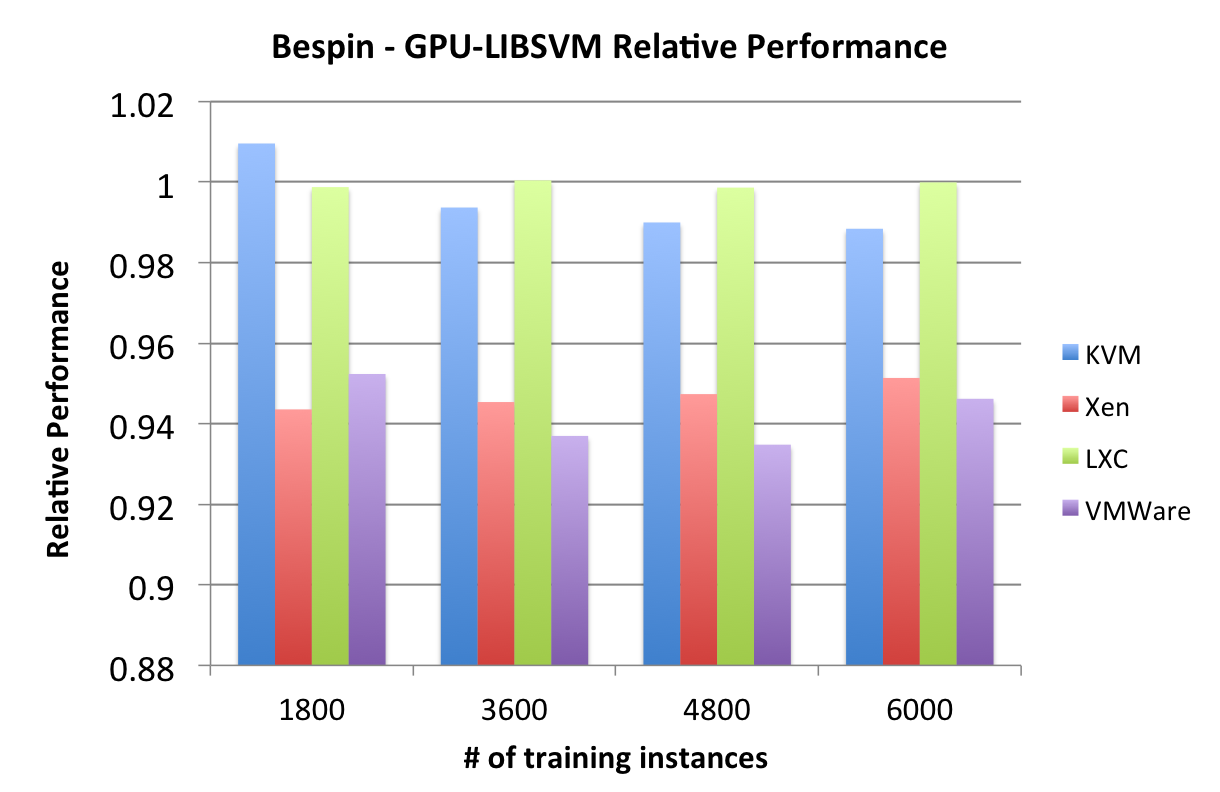
\includegraphics[width=3.25in]{figures/libSVM}}
%\caption{GPU-LIBSVM relative performance on Bespin system.  Higher is better.}
%\label{LIBSVM}
%\end{figure}

%\begin{figure}[ht!]
%\centering
%\fbox{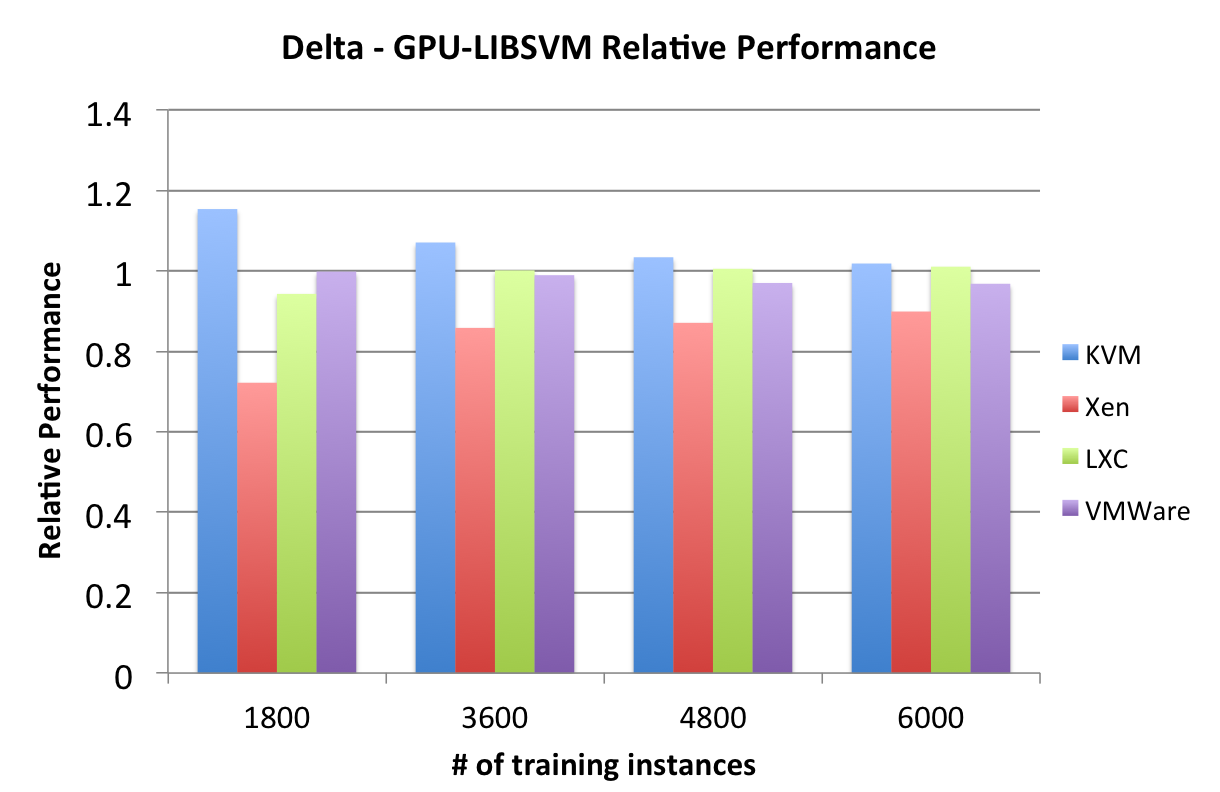
\includegraphics[width=3.25in]{figures/delta-libsvm-rel.png}}
%\caption{GPU-LIBSVM relative performance on Delta showing improved performance
%within virtual environments.  Higher is better.}
%\label{delta-LIBSVM}
%\end{figure}

In Figures~\ref{F:LIBSVM} and~\ref{F:delta-LIBSVM}, we display our GPU-LIBSVM performance results for the
Bespin (K20m) and Delta (C2075) systems. Using the NIPS 2003 gisette data set, we show the
performance across 4 problems sizes, ranging from 1800 to 6000 training
instances. The NIPS 2003 gisette dataset is a standard dataset that was used as a part of
the NIPS 2003 feature selection challenge. 

KVM again performs well across both the Delta and Bespin systems.  In the case
of the Delta system, in fact, KVM, significantly outperforms the base
system.  We determined this to be caused by KVM's support for transparent
hugepages.  When sufficient memory is available, transparent hugepages may be
used to back the entirety of the guest VM's memory.  Hugepages have previously
been shown to improve TLB performance for KVM guests, and have been shown to
occasionally boost the performance of a KVM guests beyond its
host~\cite{Arcangeli:2010}.  After disabling hugepages on the KVM host for the
Delta system, performance dropped to 80--87\% of the base system, suggesting that
memory optimizations such as transparent hugepages can substantially improve the
performance of virtualized guests under some circumstances.  LXC and VMWare
perform close to the base system, while Xen achieves between 72--90\% of the
base system's performance.  We speculate that this may be related to Xen's
inability to enabled page sizes larger than 4k.

%Another unusual characteristic of the
%GPU-LIBSVM benchmarks is that LXC performs unusually poorly for small problem
%sizes on the Delta system.  This effect is not apparent on the Bespin system,
%and its cause on the Delta system is under investigation. Xen performs comparably across both systems, ranging from 96 - 99\% efficiency
%in the case of Bespin, and maintaining 96\% efficiency on the Delta system.  

%GPU-LIBSVM is unique among our studied benchmarks,
%  in that the virtualization layer itself improves
%performance in the case of KVM and VMWare.  We explore this in more detail in
%Section~\ref{OVERHEADS}.


%This is accomplished through the use of
%transparent hugepages (THP), which are known to improve TLB performance for KVM
%guests~\cite{LINUXCONF}.  In some cases, this has resulted in improved performance over the base
%system~\cite{LINUXCONF}.  VMWare ESXi supports a related technology, Superpages;
%and as we show in Figure~\ref{delta-LIBSVM}, VMWare is also capable of
%ourperforming the base system, especially for small problem sizes.  

%The degree of performance boost depends largely on the problem size and system
%architecture.  In the case of our Bespin system, hugepages result in only a
%slight performance boost, and only for the smallest problem size.  In the case
%of the Delta system, however, performance boosts of nearly 40\% for KVM, and
%20\% for VMWare are possible.  While the effect of hugepages and superpages
%decreases for increasing problem sizes, there is still a noticeable impact on
%Delta for hugepages at all problem sizes.  When disabling transparent hugepages;
%however, performance returns to XXXSOMETHINGXXX, comparable with the host.

%For the smallest problem size of 1800 (XXXSOMETHINGSXXX), the use of THP boosts
%performance slightly higher than the base system.  The improvement disappears
%both as problem sizes increase, and when THP are disabled.  In
%Figure~\ref{LIBSVM}, we provide performance both for hugepages enabled and
%disabled for the KVM hypervisor.      

\subsection{LAMMPS Performance}

\FIGURE{!htb}
  {images/rhodo}
  {1.0}
  {LAMMPS Rhodopsin benchmark relative performance for Bespin system.  Higher is better.}
  {F:RHODO} 


\FIGURE{!htb}
  {images/delta-lammps-rhodo}
  {1.0}
  {LAMMPS Rhodopsin benchmark relative performance for Delta system.  Higher is better.}
  {F:delta-RHODO} 


%\begin{figure}[ht!]
%\centering
%\fbox{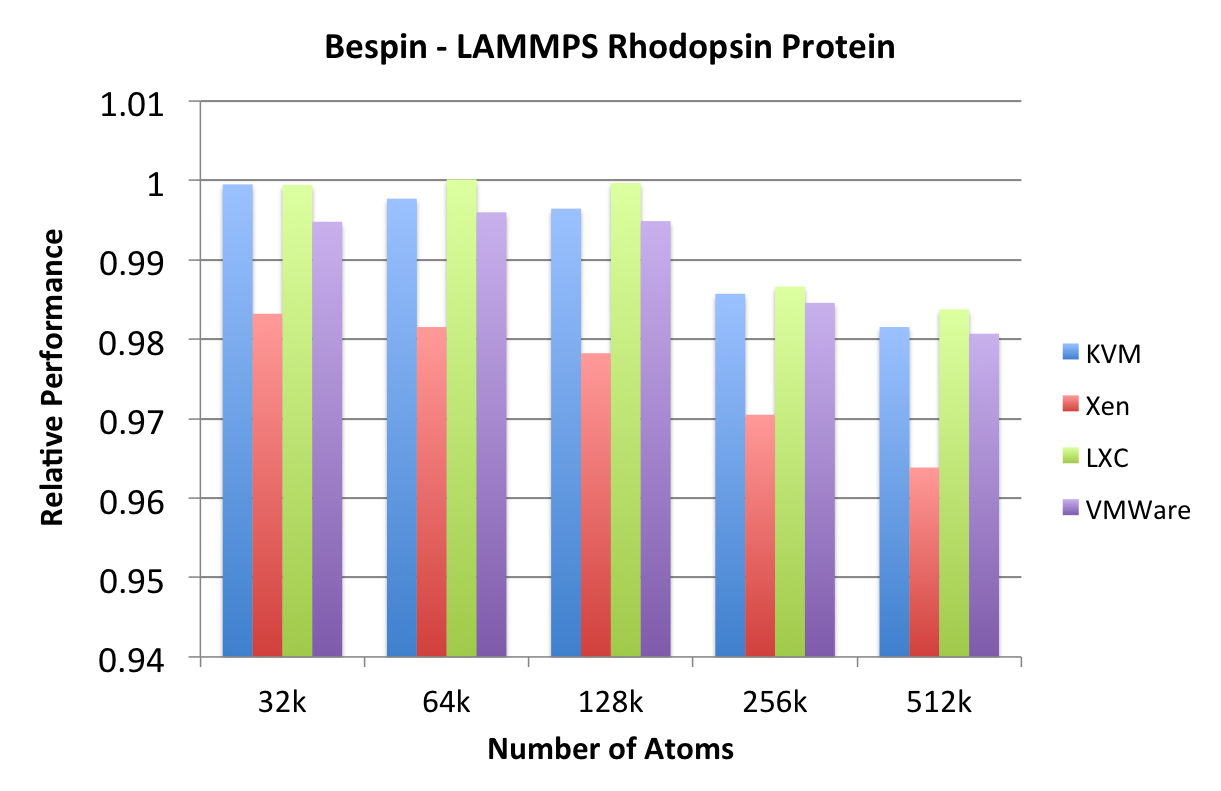
\includegraphics[width=3.25in]{figures/rhodo}}
%\caption{LAMMPS Rhodopsin benchmark relative performance for Bespin system.  Higher is better.}
%\label{RHODO}
%\end{figure}


%\begin{figure}[ht!]
%\centering
%\fbox{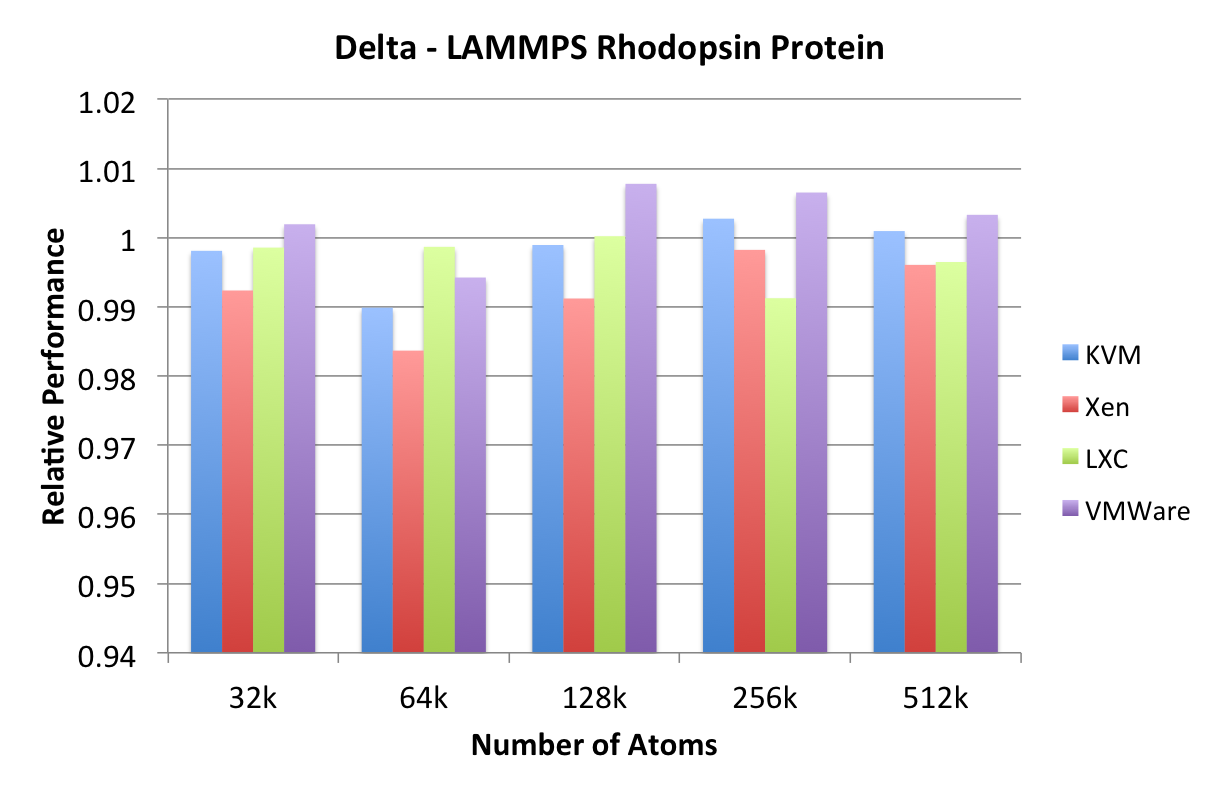
\includegraphics[width=3.25in]{figures/delta-lammps-rhodo}}
%\caption{LAMMPS Rhodopsin benchmark relative performance for Delta system.  Higher is better.}
%\label{delta-RHODO}
%\end{figure}

In Figures~\ref{F:RHODO} and~\ref{F:delta-RHODO}, we show the LAMMPS Rhodopsin protein simulation results.
LAMMPS is unique among our benchmarks, in that it exercises both the GPU and
multiple CPU cores.  In keeping with the LAMMPS benchmarking methodology, we
execute the benchmark using 1 GPU and 1--8 CPU cores
on the Bespin system,
selecting the highest performing configuration.  In the case of the Delta
system, we execute the benchmark on 1--6 cores and 1 GPU, selecting the highest
performing configuration.

Overall, LAMMPS performs well across both hypervisors and systems.
Surprisingly, LAMMPS showed better efficiency on the Delta system than the
Bespin system, achieving greater than 98\% efficiency across the board, while
Xen on the Bespin system occasionally drops as low as 96.5\% efficiency. 

This performance is encouraging because it suggests that even heterogeneous CPU
+ GPU code is capable of performing well in a virtualized environment.  Unlike
SHOC, GPU-LIBSVM, and LULESH, LAMMPS fully exercises multiple host CPUs,
splitting work between one or more GPUs and one or more CPU cores.  This has the
potential to introduce additional performance overhead, but the results do not
bear this out in the case of LAMMPS.  

%As the problem size (number of atoms) increases, LAMMPS is able to more
%effectively use a greater number of CPU cores.  Between 32k and 128k atoms, 4
%and 6 cores are the highest performing configurations.  This results in greater
%than 99\% efficiency for all but the Xen hypervisor.  

%There is a slight decrease in efficiency at 256k and 512k atom configurations.
%These configurations use all 8 CPU cores available to the VM.  The apparent
%overhead is unrelated to virtualization.  Instead, it is simply due to the host
%system offloading operating system tasks to the 8 additional cores and
%dedicating a full 8 cores to LAMMPS, while the virtual machines' 8 cores
%balanced LAMMPS computation and other operating system-related tasks.  This is
%not an overhead due to virtualization, but rather a resource advantage on the
%part of the host system.  Restricting the base system to 8 cores and 24G RAM,
%resulted in performance comparable to the virtual machines.

\subsection{LULESH Performance}

In Figure~\ref{F:LULESH_bespin} we present our LULESH results for problem sizes
ranging from mesh resolutions of $N=30$ to $N=150$.  LULESH is a highly compute-intensive
simulation, with limited data movement between the host/virtual machine and the
GPU, making it ideal for GPU acceleration. Consequently, we would expect
little overhead due to virtualization. We show LULESH results only on the Bespin
system, because differences in the code bases between the Kepler and Fermi
implementations led to unsound comparisons.

While, overall, we see very little overhead, there is a
slight scaling effect that is most apparent in the case of the Xen hypervisor.
As the mesh resolution ($N^3$) increases from $N=30$ to $N=150$, we see that the Xen
overhead decreases until Xen performs on-par with
KVM, LXC, and VMWare.  


\FIGURE{!htb}
  {images/LULESH_bespin}
  {1.0}
  {LULESH relative performance on Bespin. Higher is better.}
  {F:LULESH_bespin} 

%\begin{figure}[ht!]
%\centering
%\fbox{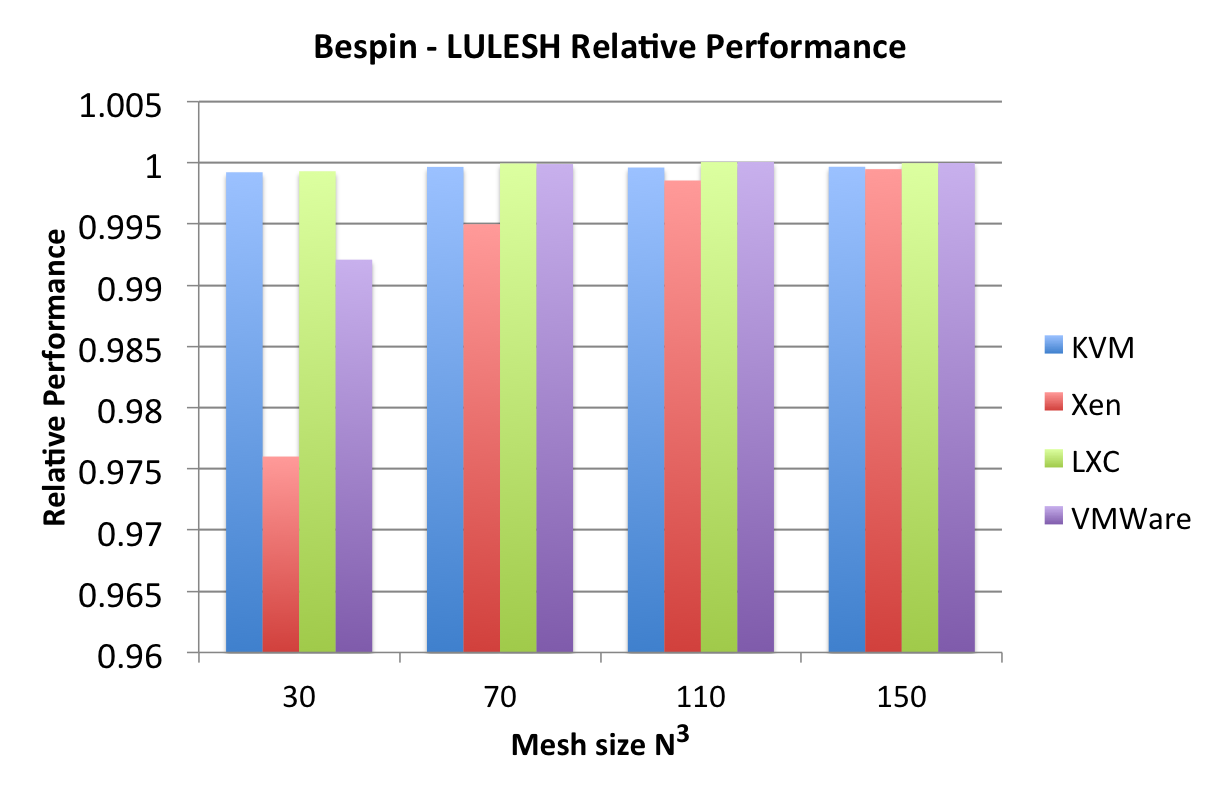
\includegraphics[width=3.25in]{figures/LULESH_bespin}}
%\caption{LULESH relative performance on Bespin. Higher is better.}
%\label{LULESH_bespin}
%\end{figure}


\section{Lessons Learned}\label{LESSONS}
%The primary lesson learned through this experiment is that in the span of a single microarchitectural generation, virtualization
%performance has improved dramatically.  While we've shown that prior processor
%generations at times impose a significant performance penalty, even when paired
%with a non-virtualized GPU, today's processors have reduced that penalty (on
%avereage) to less than 1\%.  

Virtualizing performance-critical workloads has always proven controversial,
whether the workload is CPU-only \cite{Younge2011cloud} or CPU with GPU.  From our Westmere results, we
can see that this criticism is in part legitimate, at times resulting in a performance
penalty of greater than 10\%, especially in the case of the VMWare ESXi and Xen
hypervisors.  We believe much of this to be fixable, especially in the case of
the Xen hypervisor.  

At the same time, however, we have shown that the Sandy Bridge
processor generation has nearly erased those performance overheads, suggesting
that old arguments against virtualization for performance-critical tasks should
be reconsidered.  In light of this, the primary lesson from this study is that VGA-passthrough to
virtual machines is achievable at low overhead, and across a variety of
hypervisors and virtualization platforms.  Virtualization performance remains
inconsistent across hypervisors for the Westmere generation of processors, but
starting with the Sandy Bridge architecture, performance and consistency
increase dramatically.  In the case of the Sandy Bridge architecture, even the lowest performing hypervisor, open source Xen, typically
performs within 95\% of the base case.

This study has also yielded valuable insight into the merits of each hypervisor.
KVM consistently yielded near-native performance across the full range of
benchmarks.  Its support for transparent hugepages resulted in slight
performance boosts over-and-above even the base CentOS system in the case of the
Delta system.  

%This was true
%across both the Delta (C2075) and Bespin (K20) systems, but the effect was much
%greater in the case of the Delta system.  

VMWare's performance proved inconsistent across architectures, performing well
in the case of Bespin, and relatively poorly in the case of the Delta system.
Because hypervisor configurations were identical across systems, we can only speculate that
VMWare's performance is aided by the virtualization improvements offered by the
Sandy Bridge microarchitecture.  

The Xen hypervisor was consistently average across both architectures,
performing neither poorly nor extraordinarily well in any individual benchmark.
Xen and VMWare ESXi are the only two hypervisors from this study that officially support VGA
passthrough.  As a result, PCI passthrough support in both Xen and VMWare is
more robust than KVM.  We expect that this advantage will not last long, as
commercial solutions targeting PCI passthrough in KVM are becoming
common, particularly with regard to SR-IOV and networking adapters.

Linux Containers (LXC), consistently performed closest to the native case.
This, of course, is not surprising given that LXC guests share a
single kernel with their hosts.  This performance comes at the cost of both
flexibility and security, however.  LXC is less flexible than its full
virtualization counterparts, offering
support for only Linux guests.  More importantly, LXC device
passthrough has security implications for multi-GPU systems.  In the case of
a multi-GPU-enabled host with NVIDIA hardware, both GPUs must be passed to the
LXC guest in order to initialize the driver.  This limitation may be addressable
in future revisions to the NVIDIA driver. 


\section{Directions for Future Work}\label{FUTURE}
In this chapter we have characterized the performance of 4 common hypervisors
across two generations of GPUs and two host microarchitectures, and across 3
sets of benchmarks.  We showed the dramatic improvement in virtualization
performance between the Fermi/Westmere and the Kepler/Sandy Bridge system, with
the Sandy Bridge system typically performing within 1\% of the base system.
Finally, this study sought to characterize the GPU and CPU+GPU performance with
carefully tuned hypervisor and guest configurations, especially with respect to
NUMA.  Improvements must be made to today's hypervisors in order
to improve virtual NUMA support. Finally, cloud infrastructure, such as OpenStack, must be capable
of automatically allocating virtual machines in a NUMA-friendly manner in order
to achieve acceptable results at cloud-scale.

%This has implications for virtualized high performance computing in addition to
%the single GPU-enabled nodes shown in this paper.

The next step in this work is to move beyond the single node to show that
clusters of accelerators can be efficiently used with minimal overhead.  This
will require studies in high speed networking, particularly SR-IOV-enabled 
ethernet and Infiniband.  Special attention is needed to ensure that
latencies remain tolerable within virtual environments.  Some studies have begun
to examine these issues~\cite{SRIOVInfiniband}, but open questions remain.


%Virtual NUMA support for the
%hypervisors in this study ranged from non-existent, to commercially supported.






 
%% Author: Andrew J. Younge
%% PhD Thesis/Project



%$$$$$$$$$$$$$$$$$$$$$$$$$$$$$$$$$$$$$$$$$$$$$$$$$$$$$$$$$$$$$$$$$$$$%
\chapter{Supporting High Performance Molecular Dynamics in Virtualized Clusters using IOMMU, SR-IOV, and GPUDirect}
\label{chap:mdsimulations}
%$$$$$$$$$$$$$$$$$$$$$$$$$$$$$$$$$$$$$$$$$$$$$$$$$$$$$$$$$$$$$$$$$$$$%

%\begin{comment}
%\begin{abstract}
%%%%%%%%%%%%%%%%%%%%%%%%%%%%%%%%%%%%%%%%%%%%%%%%%%%%%%%%%%%%%%%%%%%%%%
\section{Abstract}
%%%%%%%%%%%%%%%%%%%%%%%%%%%%%%%%%%%%%%%%%%%%%%%%%%%%%%%%%%%%%%%%%%%%%%
Cloud infrastructure-as-a-Service paradigms have recently shown their utility for a vast array of computational problems, ranging from advanced web service architectures to high throughput computing.  However, many scientific computing applications have been slow to adapt to virtualized cloud frameworks. This is due to performance impacts of virtualization technologies, coupled with the lack of advanced hardware support necessary for running many high performance scientific a:tabnpplications at scale. 

By using KVM virtual machines that leverage both Nvidia GPUs and InfiniBand, we show that molecular dynamics simulations with LAMMPS and HOOMD run at near-native speeds. This experiment also illustrates how virtualized environments can support the latest parallel computing paradigms, including both MPI+CUDA and new GPUDirect RDMA functionality. Specific findings show initial promise in scaling of such applications to larger production deployments targeting large scale computational workloads.  


%While these experiments do go beyond a single-node, their early implementation is limited to only 4 nodes due to the lack of feasible resources. Currently efforts are under way to scale the deployment to hundreds of cores and 32 GPUs within the FutureGrid testbed, which we look to demonstrate at Supercomputing 2014 in November. 
 

%and Cloud IaaS platforms may be well suited for supporting larger scale scientific applications, including support for the long tail of science. 

%* High performance Cloud IaaS \\
%* Support mid-tier scientific computing \\
%* Long tail of science \\
%* MD simulations \\
%* Good results \\

%\end{abstract}
%\end{comment}

\section{Introduction}

At present we stand at the inevitable intersection between High Performance Computing (HPC) and clouds. Various platform tools such as Hadoop and MapReduce, among others, have already percolated into data intensive computing within HPC~\cite{Jha2014apache}.  In addition, there are efforts to support traditional HPC-centric scientific computing applications in virtualized cloud infrastructure.  There are a multitude of reasons for supporting parallel computation in the cloud\cite{Armbrust2010}, including features such as dynamic scalability, specialized operating environments, simple management interfaces, fault tolerance, and enhanced quality of service, to name a few. The growing importance of supporting advanced scientific computing using virtualized infrastructure can be seen by a variety of new efforts, including the NSF-funded Comet resource part of XSEDE at San Diego Supercomputer Center \cite{moore2014gateways}.  

Nevertheless, there exists a past notion that virtualization used in today's cloud infrastructure is inherently inefficient.  Historically, cloud infrastructure has also done little to provide the necessary advanced hardware capabilities that have become almost mandatory in supercomputers today, most notably advanced GPUs and high-speed, low-latency interconnects.  The result of these notions has hindered the use of virtualized environments for parallel computation, where performance must be paramount.

A growing effort is currently underway that looks to systematically identify and
reduce any overhead in virtualization technologies. This effort has, thus far,
proven to be a qualified success~\cite{Younge2011cloud, Luszczek:2011:EHC}, though further research is needed to address
issues of scalability and I/O.  Thus, we see a constantly diminishing overhead
with virtualization, not only with traditional cloud workloads
\cite{huber2011evaluating} but also with HPC workloads.  While virtualization
will almost always include some additional overhead in relation to its dynamic
features, the eventual goal for supporting HPC in virtualized environments is to
minimize what overhead exists whenever possible.  To advance the placement of
HPC applications on virtual machines, new efforts are emerging which focus
specifically on key hardware now commonplace in supercomputers. By leveraging
new virtualization tools such as IOMMU device passthrough and SR-IOV, we can now
support the such advanced hardware as the latest Nvidia Tesla GPUs
\cite{Walters2014cloud}  as well as InfiniBand fabrics for high performance networking
and I/O~\cite{jose2013sr,Musleh2014cloud}.  

With the advances in hypervisor performance coupled with the newfound availability of HPC hardware in virtual machines analogous to the most powerful supercomputers used today, we see can see the possibility of a high performance cloud infrastructure using virtualization. While our previous efforts in this area have focused on single-node advancements, it is now imperative to ensure real-world applications can also operate in distributed environments as found in today's cluster and cloud infrastructures. 

Efforts to improve power efficiency and performance in data centers has led to more heterogeneous architectures. That move toward heterogeneity has, in turn, led to support for heterogeneity in the cloud. For example, Amazon EC2 supports GPU accelerators in EC2~\cite{www-amazon-gpu}, and OpenStack supports heterogeneity using flavors~\cite{www-openstack-flavors}. These advancements in cloud-level support for heterogeneity combined with better support for high-performance virtualization makes the use of cloud for HPC much more feasible for a wider range of applications and platforms.

In this paper we describe background a related work. Then, we describe a heterogeneous cloud platform, based on OpenStack. This
effort has been under development at USC/ISI since 2011~\cite{crago2011heterogeneous}.
We describe our work towards integrating GPU and InfiniBand support into
OpenStack, and we describe the heterogeneous scheduling additions that are
necessary to support not only attached accelerators, but any cloud composed of
heterogeneous elements.  

We then demonstrate running two molecular dynamics simulations, LAMMPS and HOOMD, in a virtual infrastructure complete with both Kepler GPUs and QDR InfiniBand.  Both HOOMD and LAMMPS are used extensively in some of the world's fastest supercomputers and represent example simulations that HPC supports today.  We show that these applications are able to run at near-native speeds within a completely virtualized environment, demonstrating just small performance impacts that are usually acceptable by many users. Furthermore, we demonstrate the ability of such a virtualized environment to support cutting edge software tools such as RDMA GPUDirect, illustrating how cutting-edge HPC technologies are also possible in a virtualized environment. 

Following these efforts, we hope to ensure upstream infrastructure projects such as OpenStack \cite{www-Openstack, pepple2011deploying} are able to make effective and quick use of these features, allowing users to build private cloud infrastructure to support high performance distributed computational workloads. 

%Furthermore, the tighet and exact integration into an open source Cloud infrastructure framework such as OpenStack also becomes a critical next step.  

%This manuscript demonstrates 


%The tight and exact integration into an open source cloud IaaS framework such as OpenStack \cite{www-openstack} becomes critical.

 

%* Broadly talk about clouds, OpenStack, some of our earlier HPC and GPU work\\
%* We've shown single node GPU performance at nearly 100\% efficieny (we'll need to be more accurate/precise than that in the actual submission). \\
%* In this work we demonstrate two molecular dynamics simuations running in a virtual infrastructure: LAMMPS and  HOOMD \\
%* We show that both perform near-native, and we show GPU Direct RDMA for the first time in the cloud \\

\section{Background and Related Work}

%NOTE: first introduce virtualization, and I/O featuresets. Then enable GPUs. Then bring in SR-IOv and infiniBand. Finally, discuss applications and GPUDirect.

Virtualization technologies and hypervisors have been seen widespread deployment in support of a vast array of applications.  This ranges from public commercial Cloud deployments such as Amazon EC2 \cite{hazelhurst2008scientific,amazon2010}, Microsoft Azure \cite{jennings2010cloud}, and Google's Cloud Platform \cite{www-google-platform} to private deployments within colocation facilities, corporate data centers, and even national scale cyber infrastructure initiatives.  All these support look to support various use cases and applications such as web servers, ACID and BASE databases, online object storage, and even distributed systems, to name a few.  

The use of virtualization and hypervisors specifically support various HPC solutions has been studied with mixed results.  In ~\cite{Younge2011cloud}, it is found that there is a great deal of variance between hypervisors when running various distributed memory and MPI applications, finding that KVM overall performed well across an array of HPC benchmarks.  Furthermore, some applications may not may fit well into default virtualized environments, such as High Performance Linpack \cite{Luszczek:2011:EHC}. Other studies have specifically looked at interconnect performance in virtualization and found the best-case scenario to be lacking \cite{Ramakrishnan2012} with up to 60\% performance penalties with conventional techniques.
 
Recently, various CPU architectures have added support for I/O virtualization mechanisms in the CPU ISA through the use of an I/O memory management unit (IOMMU). Often, this is referred to as PCI Passthrough, as it enabled devices on the PCI-Express bus to be passed directly to a specific virtual machine (VM).  Specific hardware implementations include Intel's VT-d \cite{intelvirtualization}, AMD's IOMMU \cite{amdiommu} from x86\_64 architectures, and even more recently ARM System MMU \cite{armmmu}.  All of these implementations effectively look to aid in the usage of DMA-capable hardware to be used within a specific virtual machine. Using these features, a wide array of hardware can be utilized directly within VMs and enable fast and efficient computation and I/O capabilities.

With PCI Passthrough, a PCI device is handed directly to a running (or booting) VM, thereby relinquishing control of the device within the host entirely. This is different from typical VM usage where hardware is emulated in the host and used in a guest VM, such as with bridged ethernet adapters or emulated VGA devices. Performing PCI Passthrough requires the host to seize the device upon boot using a specialized driver to effectively block normal driver initialization. In the instance of the KVM hypervisor, this is done using the \emph{vfio} and \emph{pci\_stub} drivers. Then, this driver relinquishes control to the VM, whereby normal device drivers initiate the hardware and enable the device for use by the guest OS.  

\subsection{GPU Passthrough}

Nvidia GPUs comprise the single most common accelerator in the Nov 2014 Top 500 List \cite{www-top500} and represent an increasing shift towards accelerators for HPC applications. Historically, GPU usage in a virtualized environment has been difficult, especially for scientific computation. Various front-end remote API implementations have been developed to provide CUDA and OpenCL libraries in VMs, which translate library calls to a back-end or remote GPU. One common use case of this is rCUDA \cite{duato2011enabling}, which provides a front-end CUDA API within a VM or any compute node, and then sends the calls via Ethernet or InfiniBand to a separate node with 1 or more GPUs. While this method is valid, it has the drawback of relying on the interconnect itself and the bandwidth available, which can be especially problematic on Ethernet. Furthermore, as this method consumes bandwidth, it can leave little remaining for MPI or RDMA routines, thereby constructing a bottleneck for some MPI+CUDA applications that depend on inter-process communication.

Recently efforts have been seen to support such GPU accelerators within VMs using IOMMU technologies, with implementations now available with KVM \cite{Walters2014cloud}, Xen \cite{Younge2014hpgc} and VMWare \cite{Vu2014}.  These efforts have shown that GPUs can achieve up to 99\% of their bare metal performance when passed to a virtual machine using PCI Passthrough.  VMWare specifically shows how the such PCI Passthrough solutions perform well and are likely to outperform front-end Remote API solutions such as rCUDA within a VM\cite{Vu2014}.  While these works demonstrate PCI Passthrough performance across a range of hypervisors and GPUs, they have been limited to investigating single node performance until now. 

\subsection{SR-IOV and InfiniBand}

With almost all parallel HPC applications, the interconnect fabric which enables fast and efficient communication between processors becomes a central requirement to achieving good performance. Specifically, a high bandwidth link is needed for distributed processors to share large amounts of data across the system. Furthermore, low latency becomes equally important for ensuring quick delivery of small message communications and resolving large collective barriers within many parallelized codes. One such interconnect, InfiniBand, has become the most common implementation used within the Top500 list. However previously InfiniBand was inaccessible to virtualized environments.  

Supporting I/O interconnects in VMs has been aided by Single Root I/O Virtualization (SR-IOV), whereby multiple virtual PCI functions are created in hardware to represent a single PCI device. These virtual functions (VFs) can then be passed to a VM and used as by the guest as if it had direct access to that PCI device. SR-IOV allows for the virtualization and multiplexing to be done within the hardware, effectively providing higher performance and greater control than software solutions. 

SR-IOV has been used in conjunction with Ethernet devices to provide high performance 10Gb TCP/IP connectivity within VMs \cite{Liu2010}, offering near-native bandwidth and advanced QoS features not easily obtained through emulated Ethernet offerings. Currently Amazon EC2 offers a high performance VM solution utilizing SR-IOV enabled 10Gb Ethernet adapters. While SR-IOV enabled 10Gb Ethernet solutions offers a big forward in performance, Ethernet still does not offer the high bandwidth or low latency typically found with InfiniBand solutions. 

Recently SR-IOV support for InfiniBand has been added by Mellanox in the ConnectX series adapters. Initial evaluation of SR-IOV InfiniBand within KVM VMs has proven has found point-to-point bandwidth to be near-native, but up to 30\% latency overhead for very small messages \cite{jose2013sr, RuivoAGTKNR14}. However, even with the noted overhead, this still signifies up to an order of magnitude difference in latency between InfiniBand and Ethernet with VMs. Furthermore, advanced configuration of SR-IOV enabled InfiniBand fabric is taking shape, with recent research showing up to a 30\% reduction in the latency overhead \cite{Musleh2014cloud}. However, real application performance has not yet been well understood until now. 

\subsection{GPUDirect}
NVIDIA's GPUDirect technology was introduced to reduce the overhead of data
movement across GPUs~\cite{GPUDirect, shainer2011development}.  GPUDirect
supports both networking as
well as peer-to-peer interfaces for single node multi-GPU systems.  The most
recent implementation of GPUDirect, version 3, adds support for RDMA over
InfiniBand for Kepler-class GPUs.

The networking component of GPUDirect relies on three key technologies: CUDA 5
(and up), a CUDA-enabled MPI implementation, and a Kepler-class GPU (RDMA only).
Both MVAPICH and OpenMPI support GPUDirect.  Support for RDMA over GPUDirect is
enabled by the MPI library, given supported hardware, and does not depend on
application-level changes to a user's code.

In this paper, our GPUDirect work focuses on GPUDirect v3 for multi-node RDMA
support.  We demonstrate scaling for up to 4 nodes connected via QDR InfiniBand
and show that GPUDirect RDMA improves both scalability and overall performance
by approximately 9\% at no cost to the end user.

\section{A Cloud for High Performance Computing}
With support for GPU Passthrough, SR-IOV, and GPUDirect, we have the building
blocks for a high performance, heterogeneous cloud.  In addition, other common
accelerators (e.g. Xeon Phi~\cite{Phi}) have similarly been demonstrated in
virtualized environments.  Our vision is of a heterogeneous cloud, supporting
both high speed networking and accelerators for tightly coupled applications.

To this end we have developed a heterogeneous cloud based on
OpenStack~\cite{www-Openstack}.  In our previous work, we
have demonstrated the ability to rapidly provision GPU, bare metal, and other
heterogeneous resources within a single cloud~\cite{crago2011heterogeneous}.
Building on this effort we have added support for GPU passthrough to OpenStack
as well as SR-IOV support for both ConnectX-2 and ConnectX-3 Infiniband devices.
Mellanox separately supports an OpenStack InfiniBand networking plugin for
OpenStack's Neutron service~\cite{ML2}, however the Mellanox plugin depends on
the ConnectX-3 adapter.  Our institutional requirements depend on ConnecteX-2
SR-IOV support, requiring an independent implementation.

OpenStack supports services for networking (Neutron), compute (Nova), identity
(Keystone), storage (Cinder, Swift), and others.  Our work focuses entirely
on the compute service.  

Scheduling is implemented at two levels: the cloud-level and the node-level.  In
our earlier work, we have developed a cloud-level heterogeneous scheduler for OpenStack,
allowing scheduling based on architectures and
resources~\cite{crago2011heterogeneous}.  In this model, the cloud-level
scheduler dispatches jobs to nodes based on resource requirements (e.g. Kepler
GPU) and node-level resource availability.

At the node, a second level of scheduling occurs to ensure that resources are
tracked and not over-committed.  Unlike traditional cloud paradigms, devices
passed into VMs cannot be over-committed.  We treat devices, whether GPUs or
InfiniBand virtual functions, as schedulable resources.  Thus, it is the responsibility of the
individual node to track resources committed and report availability to the
cloud-level scheduler.  For reporting, we piggyback on top of OpenStack's
existing reporting mechanism to provide a low overhead solution.


\section{Benchmarks}
We selected two molecular dynamics (MD) applications for evaluation in this study:
LAMMPS and HOOMD~\cite{plimpton2007lammps,anderson2010hoomd}.  These MD simulations are chosen to represent a subset of advance parallel computation for a number of fundamental reasons:

\begin{itemize}
\item MD simulations provide a practical representation of N-Body simulations, which is one of the major computational \emph{Dwarfs} \cite{asanovic2006landscape} in parallel and distributed computing. 
\item MD simulations are one of the most widely deployed applications on large scale supercomputers today.
\item Many MD simulations have a hybrid MPI+CUDA programming model, which has often become commonplace in HPC as the use of accelerators increases.
\end{itemize}

As such, we look to LAMMPS and HOOMD to provide a real-world example for running cutting-edge parallel programs on virtualized infrastructure. While these applications by no means represent all parallel scientific computing efforts (as justified by the 13 Dwarfs defined in \cite{asanovic2006landscape}), we hope these MD simulators offer a more pragmatic viewpoint than traditional synthetic HPC benchmarks such as High Performance Linpack. 

\paragraph {LAMMPS} The Large-scale Atomic/Molecular Parallel Simulator is a
well understood highly parallel molecular dynamics simulator.  It supports both
CPU and GPU-based workloads.  Unlike many simulators, both MD and otherwise,
LAMMPS is heterogeneous.  It will use both GPUs and multicore CPUs concurrently.
For this study, this heterogeneous functionality introduces additional load on
the host, allowing LAMMPS to utilize all available cores on a given system.
Networking in LAMMPS is accomplished using a typical MPI model. That is, data is
copied from the GPU back to the host and sent over the InfiniBand fabric.  No
RDMA is used for these experiments.  

\paragraph{HOOMD-blue} The Highly Optimized Object-oriented Many-particle
Dynamics -- Blue Edition is a particle dynamics simulator capable of
scaling into the thousands of GPUs.  HOOMD supports executing on both CPUs and
GPUs.  Unlike LAMMPS, HOOMD is homogeneous and does not support mixing
of GPUs and CPUs.  HOOMD supports GPUDirect using a CUDA-enabled MPI.
In this paper we focus on HOOMD's
support for GPUDirect and show its benefits for increasing cluster sizes.  




%Similarly, Infiniband SR-IOV (Single Root I/O Virtualization) has been evaluated within the context of microbenchmarks~\cite{SRIOVInfiniband,Musleh2014cloud}, but performance for real applications is not yet well-understood.

%moved to related work. right placement?
%Recent work recent work has focused on single-node performance.  In \cite{walters2014}, we've shown how the latest Kepler GPUs from Nvidia  with Sandy-Bridge Intel Xeon CPUs can perform at near-native performance running various workloads across wide range of hypervisors. Furthermore, advanced configuration of SR-IOV enabled Infiniband fabric has taken shape, with recent research showing up to a 30\% reduction latency \cite{musleh2014}.  



\section{Experimental Setup}

Using two molecular dynamics tools, LAMMPS\cite{plimpton2007lammps} and HOOMD~\cite{anderson2010hoomd}, we demonstrate a high performance \textit{system}.  That is, we combine PCI passthrough for Nvidia Kepler-class GPUs with QDR Infiniband SR-IOV and show that high performance molecular dynamics simulations are achievable within a virtualized environment. 

For the first time, we also demonstrate Nvidia GPUDirect technology within such a virtual environment.  Thus, we look to not only illustrate that virtual machines provide a flexible high performance infrastructure for scaling scientific workloads including MD simulations, but also that the latest HPC features and programming environments are also available in this same model.   

\subsection{Node configuration}

To support the use of Nvidia GPUs and InfiniBand within a VM, specific and exact host configuration is needed. This node configuration is illustrated in Figure \ref{F:passthrough}.  While our implementation is specific to the KVM hypervisor, this setup represents a design that can be hypervisor agnostic.

\FIGURE{!htb}
  {images/host-pci-passthrough.png}
  {1.0}
  {Node PCI Passthrough of GPUs and InfiniBand}
  {F:passthrough}


Each node in the testbed uses CentOS 6.4 with a 3.13 upstream Linux kernel for the host OS, along with the latest KVM hypervisor, QEMU 2.1, and the \emph{vfio} driver.  Each Guest VM runs CentOS 6.4 with a stock 2.6.32-358.23.2 kernel. A Kepler GPU is passed through using PCI Passthrough and directly initiated within the VM via the Nvidia 331.20 driver and CUDA release 5.5. While this specific implementation used only a single GPU, it is also possible to include as many GPUs as one can fit within the PCI Express bus if desired. As the GPU is used by the VM, an on-board VGA device was used by the host and a standard Cirrus VGA was emulated in the guest OS. 

With using SR-IOV, the OFED drivers version 2.1-1.0.0 are used with Mellanox ConnectX-3 VPI adapter with firmware 2.31.5050.  The host driver initiates 4 VFs, one of which is passed through to the VM where the default OFED mlnx\_ib drivers are loaded.  

%The native bare-metal base system and all guest VMs are composed of a CentOS 6.4 installation with a 2.6.32-358.23.2 stock kernel, MVAPICH 2.0 GDR, and CUDA version 5.5. Each guest was allocated 20 GB of RAM and a full socket (8 cores) as well as a single InfiniBand virtual function  and 1 Kepler GPU per VM.  


%CentOS 6.4 with a 3.13 upstream Linux kernel was used as the host OS with the KVM hypervisor.  The native bare-metal base system and all guest VMs are composed of a CentOS 6.4 installation with a 2.6.32-358.23.2 stock kernel, MVAPICH 2.0 GDR, and CUDA version 5.5. Each guest was allocated 20 GB of RAM and a full socket (8 cores) as well as a single InfiniBand virtual function  and 1 Kepler GPU per VM.  

\subsection{Cluster Configuration}

Our test environment is composed of 4 servers each with a single Nvidia
Kepler-class GPU.  Two servers are equipped with K20 GPUs, while the other two
servers are equipped with K40 GPUs, demonstrating the potential for a more
heterogeneous deployment.  Each server is composed of 2 Intel Xeon E5-2670 CPUs,
48GB of DDR3 memory, and Mellanox ConnectX-3 QDR InfiniBand.  CPU sockets and
memory are split evenly between the two NUMA nodes on each system. All
InfiniBand adapters use a single Voltaire 4036 QDR switch with a software subnet
manager for IPoIB functionality.   


For these experiments, both the GPUs and InfiniBand adapters are attached to NUMA node 1 and both the guest VMs and the base system utilized identical software stacks.  Each guest was allocated 20 GB of RAM and a full socket of 8 cores, and pinned to NUMA node 1 to ensure optimal hardware usage. While all VMs are capable of login via the InfiniBand IPoIB setup, a 1Gb Ethernet network was used for all management and login tasks.  

%Our test environment is composed of 4 servers each with a single Nvidia Kepler-class GPU.  Two servers are equipped with K20 GPUs, while the other two servers are equipped with K40 GPUs, demonstrating the potenti

For a fair and effective comparison, we also use a native environment without any virtualization. This native environment employs the same hardware configuration, and like the Guest OS runs CentOS 6.4 with the stock 2.6.32-358.23.2 kernel. 

%In order to effectively test MD simulations in LAMMPS and HOOMD beyond single-node tests, ronment.  Bespin includes 4 blades, each with 2 Intel Xeron E5-2670 CPUs, 48Gb DDR3 memory, Mellanox ConnectX3 QDR InfiniBand cards, and a mixture of Nvidia Kepler series K20 and K40 GPUs.  While the effective experimental hardware allocation remains relatively low compared to production runs of either application, it does allow for a useful evaluation at a larger scale than preivously evaluated as well as a valued extrapolation to larger resources.

 
\section{Results}

In this section, we discuss the performance of both the LAMMPS and HOOMD molecular dynamics simulation tools when running within a virtualized environment. Specifically, we scale each application to 32 cores and 4 GPUs, both in a native bare-metal and virtualized environments.  Each application set was run 10 times, with the results averaged accordingly. 

\subsection{LAMMPS}

\FIGURE{!htb}
  {images/lammps-lj-scale.png}
  {1.0}
  {LAMMPS LJ Performance}
  {F:lammps-lj}


Figure~\ref{F:lammps-lj} shows one of the most common LAMMPS algorithms used; the Lennard-Jones potential (LJ).  This algorithm is deployed in two main configurations - a 1:1 core to GPU mapping, and a 8:1 core to GPU mapping.  With the LAMMPS GPU implementation, a delicate balance between GPUs and CPUs is required to find the optimal ratio for fastest computation, however here we just look at the two most obvious choices. With small problem sizes, the 1:1 mapping outperforms the more complex core deployment, as the problem does not require the additional complexity provided with multi-core solution.  As expected the multi-core configuration quickly offers better performance for larger problem sizes, achieving roughly twice the performance with all 8 available cores. This is largely due to the availability of all 8 cores to keep the GPU running 100\% with continual computation.
 
The important factor for this manuscript is the relative performance of the virtualized environment. From the results, it is clear the VM solution performs very well compared to the best-case native deployment. For the multi-core configuration across all problem sizes, the virtualized deployment averaged 98.5\% efficiency compared to native. The single core per GPU deployment reported better-than native performance at 100\% native.  This is likely due to caching effects, but further investigation is needed to fully identify this occurrence. 

 %and the Rhodopsin protein in solvated lipid bilayer benchmark (Rhodo), both running with the GPU package across 8 cores per GPU. Here we see that both benchmarks scale remarkably well in the virtualized KVM guest environment. 
%Compared to the base system performance, the VMs running LAMMPs acheive 96.7\% and 99.3\% efficiency for LJ and Rhodo, respectively when running across all nodes.  These low overheads illustrate the utility of running LAMPS on cloud infrastructure, and also hold promise for other hybrid MPI + CUDA applications to also scale well in a virtualized environment. 


Another common LAMMPS algorithm, the Rhodopsin protein in solvated lipid bilayer benchmark (Rhodo), was also run with results given in Figure \ref{F:lammps-rhodo}. As with the LJ runs, we see the multi-core to GPU configuration resulting in higher computational performance for the larger problem sizes compared to the single core per GPU configuration, as expected.  

\FIGURE{!htb}
  {images/lammps-rhodo-scale.png}
  {1.0}
  {LAMMPS RHODO Performance}
  {F:lammps-rhodo}

Again, the overhead of the virtualized configuration remains low across all configurations and problem sizes, with an average 96.4\% efficiency compared to native. Interestingly enough, we also see the performance gap decrease as the problem size increases, with the 512k problem size in yielding 99.3\% of native performance.  This finding leads us to extrapolate that a virtualized MPI+CUDA implementation would scale to a larger computational resource with similar success. 


\subsection{HOOMD}




% Compared to the base system's performance, we see overheads of 3.2\% and 0.6\% for the LJ and Rhodo benchmarks, respectively, when running 8 cores per GPU at experimental scale. 


In Figure~\ref{F:HOOMD} we show the performance of a Lennard-Jones liquid simulation with 256K particles running under HOOMD.  HOOMD includes support for CUDA-aware MPI implementations via GPUDirect.  The MVAPICH 2.0 GDR implementation enables a further optimization by supporting RDMA for GPUDirect. From Figure~\ref{F:HOOMD} we can see that HOOMD simulations, both with and without GPUDirect, perform very near-native.  The GPUDirect results at 4 nodes achieve 98.5\% of the base system's performance.  The non-GPUDirect results achieve 98.4\% efficiency at 4 nodes. These results indicate the virtualized HPC environment is able to support such complex workloads. While the effective testbed size is relatively small, it indicates that such workloads may scale equally well to hundreds or thousands of nodes. 

\FIGURE{!htb}
  {images/hoomd.png}
  {1.0}
  {HOOMD LJ Performance with 256k Simulation}
  {F:HOOMD}


\section{Discussion}

From the results, we see the potential for running HPC applications in a virtualized environment using GPUs and InfiniBand interconnect fabric. Across all LAMMPS runs with ranging core configurations, we found only a 1.9\% overhead between the KVM virtualized environment and native. For HOOMD, we found a similar 1.5\% overhead, both with and without GPU Direct. These results go against conventional wisdom that HPC workloads do not work in VMs. In fact ,we show two N-Body type simulations programmed in an MPI+CUDA implementation perform at roughly near-native performance in tuned KVM virtual machines.  

With HOOMD, we see how GPUDirect RDMA shows a clear advantage over the
non-GPUDirect implementation, achieving a 9\% performance boost in both the
native a virtualized experiments.  While GPUDirect's performance impact has been well evaluated previously \cite{GPUDirect}, it is the author's belief that this manuscript represents the first time GPUDirect has has been utilized in a virtualized environment.  

Another interesting finding of running LAMMPS and HOOMD in a virtualized environment is as workload scales from a single node to 32 cores, the overhead does not increase. These results lend credence to the notion that this solution would also work for a much larger deployment. Specifically, it would be possible to expand such computational problems to a larger deployment in FutureGrid \cite{fox2013futuregrid}, Chameleon Cloud \cite{www-chameleon}, or even the planned NSF Comet machine at SDSC, scheduled to provide up to 2 Petaflops of computational power. Effectively, these results help support the theory that a majority of HPC computations can be supported in virtualized environment with minimal overhead. 


\section{Chapter Summary}

With the advent of cloud infrastructure, the ability to run large-scale parallel scientific applications has become possible but limited due to both performance and hardware availability concerns. In this work we show that advanced HPC-oriented hardware such as the latest Nvidia GPUs and InfiniBand fabric are now available within a virtualized infrastructure. Our results find MPI + CUDA applications such as molecular dynamics simulations run at near-native performance compared to traditional non-virtualized HPC infrastructure, with just an averaged 1.9\% and 1.5\% overhead for LAMMPS and HOOMD, respectively. Moving forward, we show the utility of GPUDirect RDMA for the first time in a cloud environment with HOOMD.  Effectively, we look to pave the way for large-scale virtualized cloud Infrastructure to support a wide array of advanced scientific computation commonly found running on many supercomputers today.  Our efforts leverage these technologies and provide them in an open source Infrastructure-as-a-Service framework using OpenStack.  




 

%% Author: Andrew J. Younge
%% PhD Thesis/Project

%$$$$$$$$$$$$$$$$$$$$$$$$$$$$$$$$$$$$$$$$$$$$$$$$$$$$$$$$$$$$$$$$$$$$%
\chapter{Future Endeavours with Virtualization}
\label{chap:future-work}
%$$$$$$$$$$$$$$$$$$$$$$$$$$$$$$$$$$$$$$$$$$$$$$$$$$$$$$$$$$$$$$$$$$$$%

%%%%%%---------------------------------------------------------------
\subsection{Live Migration Mechanisms}
%%%%%%---------------------------------------------------------------

TODO: Definition of Migration, live migration, differences. (assumed known here).

Live migration of VMs represents one of the fundamental advantages to virtualization, and also one of the greatest challenges to efficiency.  In Live migration, the complete VM state is copied from a source to a unallocated destination host, where disk, memory, and network connections are kept intact. For disk continuity, a distributed and/or shared filesystem is utilized, most commonly NFS, where both the source and destination hosts have access to the Vm disk.  Network continuity is preserved so long as the destination guest is within the same LAN and generates an unsolicited ARP reply to maintain the original IP after migration.  VM vCPU states and machine states are recorded from the source and quickly sent to the destination host when the VM is paused. This pause and tranfer time represents the entirety of a VM downtime during live migration, and is often < 100 milliseconds across  commodity Ethernet networks. 

However, VM memory migration often requires the most care and is often the leading cause for migration overhead during live migration. This is due to not only the potentially large amount of memory to be sent across the network.  This is defined directly by the amount of main memory allocated (or in use) by the source VM. However, as a VM's memory is sent, the VM is still runing and therefor memory pages can be dirtied, creating the need for any written page to be retransmitted. Given a small network and a memory bound processes running within a VM, this can be an infinitely long process of page dirtying. 

A few general memory live migration concepts have been utilized, and are summarized in Figure X. 

\begin{itemize}
\item Pre-copy Migration:  All memory pages are transmitted to the destination before the VM is paused. The hypervisor will note and track all dirtied memory pages, and retransmit those pages in iterative rounds. The rounds end when either no dirtied pages exist or a max iteration count has been reached. The VM state is then transmitted and resumed on the destination. 
\item Post-copy Migration: The Vm state is immediately paused and sent to the destination hypervisor, and immediately resumed. If the new destination VM generates a page fault, the VM is paused, and faulted pages are transmitted across the network on demand from the source and the VM resumed.  
\item Hybrid-copy Migration: Provides a compromise solution to memory paging. First, single copy of the VM memory pages, or a subset of known-necessary memory pages are sent to the destination.  Then the source VM is paused, its VM state sent to the destination, and resumed on the destination.  Known dirtied source pages, or missing pages are then copied to the destination upon a triggered page fault utilizing the same mechanism as post-copy migration. 
\end{itemize}


%%%%%%---------------------------------------------------------------
\subsection{RDMA \& VMs}
%%%%%%---------------------------------------------------------------

TODO: Discuss work in \cite{huang2007high} and how we build upon the idea


%%%%%%---------------------------------------------------------------
\subsection{Fast VM Cloning}
%%%%%%---------------------------------------------------------------

In many distributed system environments, concurrency is achieved through the use of homogeneous compute nodes that handle the bulk of the computational load in parallel. In virtual clusters, there is a need to efficiently deploy and manage near identical virtual machines for distributed computation. 

In Snowflock \cite{lagar2009snowflock, lagar2011snowflock}, the notion of VM cloning is given. Specifically, Lagar et al. define the notion of VM Fork, where VMs are treated similar to a fork\(\) system call for processes.   This process is conceptually similar to VM migration, with the exception that the source VM is not destroyed after the migration. Starting with a master VM, an impromptu cluster can be created across a network using the Xen hypervisor.  Snowflock specifically uses Multicast to linearly scale out VM creation to many hosts, only coping a minimal state and then remotely coping memory pages when requested.  This fetched memory on-demand is similar in principal to the post-copy live migration technique describe in Section 3.1.  This is further augmented with blocktap-based virtual disks with Copy-on-Write (CoW) functionally, delivering CoW slices for each child VM. 

While Snowflock provides an excellent framework for VM cloning, it is not suitable for the current implementation. First, it uses Xen, which previous research has found to have limited performance for HPC workloads \cite{Younge2011cloud}.  Second, SnowFlock is designed for Ethernet and IP based networks, which have significantly higher latency and lower bandwidth when compared to InfiniBand solutions. As such, we proposed to develop analogous mechanisms on KVM to use RDMA for VM memory and disk paging. 

Potential VM Cloning RDMA mechanism:
\begin{itemize}
\item Prepare parent VM state, including registers and info
\item Create large buffers for all VM memory on child hosts (as per usual)
\item Send vmstate via RDMAwrite or IB Send to N child nodes, where N is the clone size
\item Resume/start child VMs in tandem. 
\item Have parent VM use RDMA multicast (unreliable connection) to send memory pages to all childs efficiently
\item If child page faults, does direct RDMAread operation for specific page. 
\item Priority given (somehow?) to RDMA requests first. 
\item Eventually, all children will have memory pages via multicast. As multicast is unreliable, delivery failure will just trigger a page fault and subsequent page sending via RDMA (yet unlikely)
\end{itemize}

This method allows for efficient multicasting of master VM memory.  It allows for direct page fault handling, while allowing child VMs to start and run immediately. Hybrid solution could also work with such a situation.  As RDMA multicast is relatively questionable, not sure how practical this method would/could be.




%% Author: Andrew J. Younge
%% PhD Thesis/Project

%$$$$$$$$$$$$$$$$$$$$$$$$$$$$$$$$$$$$$$$$$$$$$$$$$$$$$$$$$$$$$$$$$$$$%
\chapter{Conclusion}
\label{chap:conc}
%$$$$$$$$$$$$$$$$$$$$$$$$$$$$$$$$$$$$$$$$$$$$$$$$$$$$$$$$$$$$$$$$$$$$%

With the advent of virtualization and the availability of virtual machines through the use of cloud infrastructure, a paradigm shift in distributed systems has occurred. Many services and applications once deployed on workstations, private servers, personal computers, and even some supercomputers have migrated to a cloud infrastructure. The reasons for this  trend toward cloud infrastructure are vast, with advantages such as increased application flexibility and scalability, the ability for providers to leverages economies of scale, and customized, on-demand user environments.  However, these reasons may not be enough to support all computational challenges within such a virtualized infrastructure.

One example where cloud infrastructure has historically been insufficient is with the support for distributed memory applications. The use of tightly coupled, parallel tasks common in High Performance Computing communities has seen a number of problems and complications when deployed in virtualized infrastructure.  While the reasons for lack of integration can be numerous, many challenges stem from two aspects; the performance impact and overhead associated with virtualization, and the lack of hardware necessary to support tightly coupled concurrent tasks.  While virtualized cloud infrastructure may not be able to aid in all HPC related activities, it is possible that if these limitations are either overcome or mitigated, virtualization may be able to offer benefits to many in the HPC community. These benefits could include dynamic resource allocation, enhanced migration and data management capabilities, or even bursting capabilities for rare event simulations, to name a few.  

This dissertation looks to evaluate virtualization's ability to support mid-tier scientific HPC applications. From the beginning, this dissertation proposes the advent of high performance virtual clusters to support advanced scientific computation, including tightly coupled HPC applications.  This dissertation's framework for building such an environment aims to identify virtualization overhead and finding solutions and best practices with performant hypervisors. This effort also includes the methodology needed for supporting advanced accelerators and interconnects common in HPC environments, to enable new class of applications in virtualized infrastructure. The framework has built into it cases for evaluating potential deployments as discussed throughout using benchmarks and real-world applications.  Furthermore, it is proposed to use the OpenStack IaaS project to encompass these components together in a unified private cloud architecture.  

%\TODO{Write a bit more here}

Chapter \ref{chap:related} studied the related research necessary for defining not only the context for virtualization and cloud computing, but also virtual clusters and the history of supercomputing.  Chapter \ref{chap:cloud2011} looked to study the applicability of various hypervisors for supporting common HPC workloads through the use of benchmarks from a single-node aspect.  This found challenges and some solutions to these workloads, and identified missing gaps that exist. 

Chapter \ref{chap:hpgc2014} started the investigation of the utility of GPUs to support mid-tier scientific applications using the Xen hypervisor. This chapter provided a proof-of-concept that, with proper configuration by utilizing the latest in hardware support, GPU passthrough is a viable model for supporting CUDA-enabled applications, a fast-growing application set. Chapter \ref{chap:cloud2014} provides an in-depth comparison of multiple hypervisors using the SHOC GPU benchmark suite, as well as a few GPU-enabled HPC applications. Here we discover our KVM implementation performs at near-native speeds and allows for effective GPU utilization, and even outperforms our previous work with the Xen hypervisor. 

Chapter \ref{chap:mdsimulations} takes the lessons learned with KVM in GPU passthrough and adds in SR-IOV InfiniBand support. This high speed, low latency interconnect represents a critical tool for supporting tightly coupled distributed memory applications. With this, a high performance virtual cluster is created. This environment supports two class-leading Molecular Dynamics simulations, LAMMPs and HOOMD-blue, and shows how both applications can not only perform at near-native speeds, but also leverage the latest HPC technologies such as GPUDirect for efficient GPU-to-GPU communication across distributed memory resources. %This framework is also enveloped in an OpenStack environment.     

Chapter \ref{chap:future-work} is an introspective look at other advancements that can be made in virtualization to support high performance virtual clusters. This chaper details the mechanisms whhereby virtual clusters leverage PCI passthrough for added hardware and I/O support, along with overhead reduction of using huge pages.  With this, methods are outlined for advanced virtualization techniques such as live migration leveraging high speed RDMA-capable interconnects, possibilities for moving VMs closer to data sources, VM cloning for fast deployment of virtual clusters themselves, and scheduling considerations for integration of high performance virtual clusters. These tools are details with the consideration of integration within the OpenStack IaaS cloud for private cyberinfrastructure deployments.


Given the efforts of this dissertation, we must evaluate the original hypothesis; can virtualized infrastructure, leveraging the practices of high performance virtual clusters as defined herein, support mid-tier scientific computing endeavors? In the beginning of Chapter 3, looking at the base case when this research started, the answer was a murky \emph{no}.  When the advances made in hypervisors, the ability to leverage accelerators such as Nvidia GPUs in Chapter 4 and 5, coupled with the addition of a high performance, low-latency interconnect in Chapter 6, and leveraging advanced tuning and hypervisor configurations with KVM, answer to the hypothesis has changed to an optimistic but skeptical \emph{yes}.  This conjecture is made by evaluating the support for a common and convoluted HPC application set of various molecular dynamics applications and observing virtualization performance overhead under 2\% when compared to native, bare metal configurations.  While more work is needed to evaluate the potential for high performance virtual clusters to scale out, the current body of research does not illuminate any architectural barriers at this time.  



%\TODO{Answer the research question, can we support HPC with virtual clusters? How could this help with big data convergence?}


%%%%%%%%%%%%%%%%%%%%%%%%%%%%%%%%%%%%%%%%%%%%%%%%%%%%%%%%%%%%%%%%%%%%%%
\section{Impact}
\label{sec:impact}
%%%%%%%%%%%%%%%%%%%%%%%%%%%%%%%%%%%%%%%%%%%%%%%%%%%%%%%%%%%%%%%%%%%%%%

This dissertation has illustrated how virtualization can be used to support HPC applications using virtual clusters.  While the example applications used herein are in relation to Molecular Dynamics, it is anticipated that this work is also equally applicable to other fields including Astronomy, High Energy Physics, Bioinformatics, and computational chemistry, to name a few. In this, it is also desirous to have these high performance virtual clusters also provide a feature-rich yet performance infrastructure to new and emerging big data science applications and platform services.  While further work will likely be necessary in storage and I/O efforts related to virtualization, the potential exists today to meet the demands of a convergent infrastructure with virtualization.   

It is also possible and likely that such applications can scale with future infrastructure deployments.  Next steps in this direction to scale out could see virtual cluster sizes increase to thousands of nodes. Virtualization efforts using the Palacios VMM were able to scale a Cray XT4 system to 4096 nodes, reporting only a ~5\% overhead \cite{lange2011minimal}. While so far we've seen slightly better results with KVM at smaller scales, it is hopeful that the same scaling may be possible with KVM on newer hardware supporting a more diverse set of user environments.  

The model for PCI passthrough illustrated throughout the dissertation may also be able to impact other hardware. First, this could include the Intel Xeon Phi (co-processor models, not the Knights Landing CPU), or some emerging FPGA implementations like the Stillwater Knowledge Processing Unit (KPU), a distributed data flow processor.  The PCI-Express SIG specification has been upgraded in version 4.0 to support larger I/O devices and accelerators with on-bus power delivery, leading to the assumptions that, for at least commodity x86 systems, there could be an increase in PCIE device utilization. The caveat to this will be if the PCIE bus is abandoned or superseded by other methods, such as System-on-Chip designs or Nvidia's NVLink effort \cite{agarwal2015unlocking} where such new designs do not take into account IOMMU virtualization.  While the HPC accelerator usage could very well wane in the wake of novel many core architectures such as Knights Landing CPUs \cite{hemmert2016trinity}, such movements have still yet to take hold within the HPC community.  

As some of the advances described in the dissertation have already made their way to the OpenStack cloud platform. It is expected that OpenStack's usage will only grow in time in both academic research and industry.  With that, it may be possible to build such a cloud infrastructure to run high performance virtual clusters at a larger scale. Applying this infrastructure, along with high level experiment management and support services, could lead to a new national scale cyberinfrastructure deployment.  In time and with further development, this could deployed within the NSF-funded XSEDE project, for example. Perhaps instead of having separated hardware for HPC systems like the XSEDE Stampede resource at UT Austin and a separate cloud infrastructure deployment for HTC computing and science gateways like IU's Jetstream, a single, unified high performance cloud infrastructure could be utilized to provide all such needs concurrently.  Furthermore, with continuing on the advantages vitualizaton provides, new distributed computing paradigms and runtime systems may still yet to be realized.   



%\appendix

%\bibliographystyle{csRIT}

\bibliographystyle{tex/IEEEtran} 
\bibliography{%
bib/ajyounge,%
bib/cyberaide-cloud,%
bib/cyberaide-www,%
bib/cyberaide-greenit,%
bib/cyberaide-grid,%
bib/cyberaide-cuda,%
bib/cyberaide-biostatistics,%
bib/all,%
bib/fg-hypervisor,%
bib/cloud2014,%
bib/lammps,%
bib/futuregrid}

\chapter{Cirriculum Vitae}

\begin{comment}


\chapter{Appendix}
\label{app:appendix}

This section provides the formal description for TBD.  
%%%%%%%%%%%%%%%%%%%%%%%%%%%%%%%%%%%%%%%%%%%%%%%%%%%%%%%%%%%%%%%%%%%%%%
\section{AppendixA}
\label{app:aa}
%%%%%%%%%%%%%%%%%%%%%%%%%%%%%%%%%%%%%%%%%%%%%%%%%%%%%%%%%%%%%%%%%%%%%%



%---------------------------------------------------------------------
\subsection{Appendix A1}

\end{comment}



\phantomsection \addcontentsline{toc}{chapter}{Index} 
\renewcommand{\baselinestretch}{1} \small \normalsize \printindex

\end{document} 

